\documentclass[11pt]{article}

\usepackage[utf8]{inputenc}
\usepackage[british]{babel}
\usepackage[left=2.2cm,right=2.2cm,top=2.2cm,bottom=2.4cm]{geometry}

% ---- Maths ----
\usepackage{amstext}
\usepackage{amssymb}
\usepackage{amsmath}
\usepackage{amsfonts}
\usepackage{mathrsfs}
%\usepackage{bm}
\IfFileExists{bbm.sty}{\usepackage{bbm}}{}  % optional; not required by macros.tex
\usepackage{nicefrac,xfrac}
\usepackage{upgreek}
\usepackage{booktabs}
\usepackage{array}
\usepackage{multirow}

% ---- Colour, graphics ----
\usepackage{xcolor}
\usepackage{graphicx}
\usepackage{pgf,tikz,pgfplots}
\pgfplotsset{compat=1.16}
\usetikzlibrary{arrows,arrows.meta,calc,math,shapes,positioning,fit,backgrounds}

\usepackage[colorlinks=true,linkcolor=blue!55!black,citecolor=green!45!black,
            urlcolor=blue!55!black]{hyperref}
\usepackage[babel=true]{csquotes}
\usepackage{textcomp}
\usepackage{longtable}
\usepackage{caption}
\usepackage{subcaption}
\usepackage{url}
\usepackage{float}
\usepackage{enumerate}
\usepackage[shortlabels]{enumitem}

% ---- Theorem environments (amsthm; lighter than the ntheorem setup of Parts I--II) ----
\usepackage{amsthm}
\theoremstyle{plain}
\newtheorem{theorem}{Theorem}[section]
\newtheorem{proposition}[theorem]{Proposition}
\newtheorem{lemma}[theorem]{Lemma}
\newtheorem{corollary}[theorem]{Corollary}
\theoremstyle{definition}
\newtheorem{definition}[theorem]{Definition}
\newtheorem{experiment}{Experiment}
\theoremstyle{remark}
\newtheorem{remark}[theorem]{Remark}
\newtheorem{claimP}{Claim}

%%%%%%%%%%%%%%%%%%%%%%%%%%%%%%%%%%%%%%%%%%%%%%%%%%%%%%%%%%%%%%%%%%%%%%%%%%%%%%%
%%  Mnemonic environments, as in Part~II.  The tag is printed in the heading
%%  and returned by \ref, so a citation carries the content of the statement
%%  rather than a number.
%%
%%      assum   {f.Bb}[bounded below]
%%      cond    {C.1}[lower bound on the radius]
%%      update  {$\Rgrad$}[radius tied to the gradient]
%%  each taking the tag as a mandatory argument and the gloss as an optional
%%  one, with the \label placed inside as usual.
%%%%%%%%%%%%%%%%%%%%%%%%%%%%%%%%%%%%%%%%%%%%%%%%%%%%%%%%%%%%%%%%%%%%%%%%%%%%%%%
\makeatletter
\newcommand{\pIII@head}[3]{%
  \par\addvspace{\topsep}%
  \noindent
  \def\@currentlabel{#2}%
  {\normalfont\bfseries #1 #2%
    \if\relax\detokenize{#3}\relax\else
      \normalfont\ (#3)%
    \fi
    \normalfont\bfseries.}%
  \nobreak\hspace{.5em}\ignorespaces
}
\newenvironment{assum}[2][]{\pIII@head{Assumption}{#2}{#1}}{\par\addvspace{\topsep}}
\newenvironment{cond}[2][]{\pIII@head{Condition}{#2}{#1}}{\par\addvspace{\topsep}}
\newenvironment{update}[2][]{\pIII@head{Update}{#2}{#1}}{\par\addvspace{\topsep}}
\makeatother

\numberwithin{equation}{section}

\usepackage[ruled,vlined]{algorithm2e}
\allowdisplaybreaks

% ---- Macros of Parts I and II ----
%%  This file will be included when we compile the final book. You can
%%  make use of the commonly used packages and commonly defined macros
%%  from here.
%%
%%  PLEASE DO NOT CHANGE THIS FILE.
%%  PLEASE DO NOT REDFINE ANY OF THE MACROS.
%%
%%  For convenience you may wish to define your own macros in your main
%%  tex file while preparing the manuscript. However, before submitting
%%  your final file for the accepted manuscript, we will ask you to replace
%%  your macros with the full commands.
%%

%% OCTOBER 2021 VERSION

% We add the following commonly used macros:

% vectors as boldsymbols:
\newcommand{\bsa}{{\boldsymbol{a}}}
\newcommand{\bsb}{{\boldsymbol{b}}}
\newcommand{\bsc}{{\boldsymbol{c}}}
\newcommand{\bsd}{{\boldsymbol{d}}}
\newcommand{\bse}{{\boldsymbol{e}}}
\newcommand{\bsf}{{\boldsymbol{f}}}
\newcommand{\bsg}{{\boldsymbol{g}}}
\newcommand{\bsh}{{\boldsymbol{h}}}
\newcommand{\bsi}{{\boldsymbol{i}}}
\newcommand{\bsj}{{\boldsymbol{j}}}
\newcommand{\bsk}{{\boldsymbol{k}}}
\newcommand{\bsl}{{\boldsymbol{l}}}
\newcommand{\bsm}{{\boldsymbol{m}}}
\newcommand{\bsn}{{\boldsymbol{n}}}
\newcommand{\bso}{{\boldsymbol{o}}}
\newcommand{\bsp}{{\boldsymbol{p}}}
\newcommand{\bsq}{{\boldsymbol{q}}}
\newcommand{\bsr}{{\boldsymbol{r}}}
\newcommand{\bss}{{\boldsymbol{s}}}
\newcommand{\bst}{{\boldsymbol{t}}}
\newcommand{\bsu}{{\boldsymbol{u}}}
\newcommand{\bsv}{{\boldsymbol{v}}}
\newcommand{\bsw}{{\boldsymbol{w}}}
\newcommand{\bsx}{{\boldsymbol{x}}}
\newcommand{\bsy}{{\boldsymbol{y}}}
\newcommand{\bsz}{{\boldsymbol{z}}}
\newcommand{\bsA}{{\boldsymbol{A}}}
\newcommand{\bsB}{{\boldsymbol{B}}}
\newcommand{\bsC}{{\boldsymbol{C}}}
\newcommand{\bsD}{{\boldsymbol{D}}}
\newcommand{\bsE}{{\boldsymbol{E}}}
\newcommand{\bsF}{{\boldsymbol{F}}}
\newcommand{\bsG}{{\boldsymbol{G}}}
\newcommand{\bsH}{{\boldsymbol{H}}}
\newcommand{\bsI}{{\boldsymbol{I}}}
\newcommand{\bsJ}{{\boldsymbol{J}}}
\newcommand{\bsK}{{\boldsymbol{K}}}
\newcommand{\bsL}{{\boldsymbol{L}}}
\newcommand{\bsM}{{\boldsymbol{M}}}
\newcommand{\bsN}{{\boldsymbol{N}}}
\newcommand{\bsO}{{\boldsymbol{O}}}
\newcommand{\bsP}{{\boldsymbol{P}}}
\newcommand{\bsQ}{{\boldsymbol{Q}}}
\newcommand{\bsR}{{\boldsymbol{R}}}
\newcommand{\bsS}{{\boldsymbol{S}}}
\newcommand{\bsT}{{\boldsymbol{T}}}
\newcommand{\bsU}{{\boldsymbol{U}}}
\newcommand{\bsV}{{\boldsymbol{V}}}
\newcommand{\bsW}{{\boldsymbol{W}}}
\newcommand{\bsX}{{\boldsymbol{X}}}
\newcommand{\bsY}{{\boldsymbol{Y}}}
\newcommand{\bsZ}{{\boldsymbol{Z}}}
% other commonly used boldsymbols:
\newcommand{\bsell}{{\boldsymbol{\ell}}}
\newcommand{\bszero}{{\boldsymbol{0}}} % vector of zeros
\newcommand{\bsone}{{\boldsymbol{1}}}  % vector of ones
% boldsymbol greeks:
\newcommand{\bsalpha}{{\boldsymbol{\alpha}}}
\newcommand{\bsbeta}{{\boldsymbol{\beta}}}
\newcommand{\bsgamma}{{\boldsymbol{\gamma}}}
\newcommand{\bsdelta}{{\boldsymbol{\delta}}}
\newcommand{\bsepsilon}{{\boldsymbol{\epsilon}}}
\newcommand{\bsvarepsilon}{{\boldsymbol{\varepsilon}}}
\newcommand{\bszeta}{{\boldsymbol{\zeta}}}
\newcommand{\bseta}{{\boldsymbol{\eta}}}
\newcommand{\bstheta}{{\boldsymbol{\theta}}}
\newcommand{\bsvartheta}{{\boldsymbol{\vartheta}}}
\newcommand{\bskappa}{{\boldsymbol{\kappa}}}
\newcommand{\bslambda}{{\boldsymbol{\lambda}}}
\newcommand{\bsmu}{{\boldsymbol{\mu}}}
\newcommand{\bsnu}{{\boldsymbol{\nu}}}
\newcommand{\bsxi}{{\boldsymbol{\xi}}}
\newcommand{\bspi}{{\boldsymbol{\pi}}}
\newcommand{\bsvarpi}{{\boldsymbol{\varpi}}}
\newcommand{\bsrho}{{\boldsymbol{\rho}}}
\newcommand{\bsvarrho}{{\boldsymbol{\varrho}}}
\newcommand{\bssigma}{{\boldsymbol{\sigma}}}
\newcommand{\bsvarsigma}{{\boldsymbol{\varsigma}}}
\newcommand{\bstau}{{\boldsymbol{\tau}}}
\newcommand{\bsupsilon}{{\boldsymbol{\upsilon}}}
\newcommand{\bsphi}{{\boldsymbol{\phi}}}
\newcommand{\bsvarphi}{{\boldsymbol{\varphi}}}
\newcommand{\bschi}{{\boldsymbol{\chi}}}
\newcommand{\bspsi}{{\boldsymbol{\psi}}}
\newcommand{\bsomega}{{\boldsymbol{\omega}}}
\newcommand{\bsGamma}{{\boldsymbol{\Gamma}}}
\newcommand{\bsDelta}{{\boldsymbol{\Delta}}}
\newcommand{\bsTheta}{{\boldsymbol{\Theta}}}
\newcommand{\bsLambda}{{\boldsymbol{\Lambda}}}
\newcommand{\bsXi}{{\boldsymbol{\Xi}}}
\newcommand{\bsPi}{{\boldsymbol{\Pi}}}
\newcommand{\bsSigma}{{\boldsymbol{\Sigma}}}
\newcommand{\bsUpsilon}{{\boldsymbol{\Upsilon}}}
\newcommand{\bsPhi}{{\boldsymbol{\Phi}}}
\newcommand{\bsPsi}{{\boldsymbol{\Psi}}}
\newcommand{\bsOmega}{{\boldsymbol{\Omega}}}

% Roman fonts:
\newcommand{\rma}{{\mathrm{a}}}
\newcommand{\rmb}{{\mathrm{b}}}
\newcommand{\rmc}{{\mathrm{c}}}
\newcommand{\rmd}{{\mathrm{d}}}
\newcommand{\rme}{{\mathrm{e}}}
\newcommand{\rmf}{{\mathrm{f}}}
\newcommand{\rmg}{{\mathrm{g}}}
\newcommand{\rmh}{{\mathrm{h}}}
\newcommand{\rmi}{{\mathrm{i}}}
\newcommand{\rmj}{{\mathrm{j}}}
\newcommand{\rmk}{{\mathrm{k}}}
\newcommand{\rml}{{\mathrm{l}}}
\newcommand{\rmm}{{\mathrm{m}}}
\newcommand{\rmn}{{\mathrm{n}}}
\newcommand{\rmo}{{\mathrm{o}}}
\newcommand{\rmp}{{\mathrm{p}}}
\newcommand{\rmq}{{\mathrm{q}}}
\newcommand{\rmr}{{\mathrm{r}}}
\newcommand{\rms}{{\mathrm{s}}}
\newcommand{\rmt}{{\mathrm{t}}}
\newcommand{\rmu}{{\mathrm{u}}}
\newcommand{\rmv}{{\mathrm{v}}}
\newcommand{\rmw}{{\mathrm{w}}}
\newcommand{\rmx}{{\mathrm{x}}}
\newcommand{\rmy}{{\mathrm{y}}}
\newcommand{\rmz}{{\mathrm{z}}}
\newcommand{\rmA}{{\mathrm{A}}}
\newcommand{\rmB}{{\mathrm{B}}}
\newcommand{\rmC}{{\mathrm{C}}}
\newcommand{\rmD}{{\mathrm{D}}}
\newcommand{\rmE}{{\mathrm{E}}}
\newcommand{\rmF}{{\mathrm{F}}}
\newcommand{\rmG}{{\mathrm{G}}}
\newcommand{\rmH}{{\mathrm{H}}}
\newcommand{\rmI}{{\mathrm{I}}}
\newcommand{\rmJ}{{\mathrm{J}}}
\newcommand{\rmK}{{\mathrm{K}}}
\newcommand{\rmL}{{\mathrm{L}}}
\newcommand{\rmM}{{\mathrm{M}}}
\newcommand{\rmN}{{\mathrm{N}}}
\newcommand{\rmO}{{\mathrm{O}}}
\newcommand{\rmP}{{\mathrm{P}}}
\newcommand{\rmQ}{{\mathrm{Q}}}
\newcommand{\rmR}{{\mathrm{R}}}
\newcommand{\rmS}{{\mathrm{S}}}
\newcommand{\rmT}{{\mathrm{T}}}
\newcommand{\rmU}{{\mathrm{U}}}
\newcommand{\rmV}{{\mathrm{V}}}
\newcommand{\rmW}{{\mathrm{W}}}
\newcommand{\rmX}{{\mathrm{X}}}
\newcommand{\rmY}{{\mathrm{Y}}}
\newcommand{\rmZ}{{\mathrm{Z}}}
% also commonly defined
\newcommand{\rd}{{\mathrm{d}}}
\newcommand{\ri}{{\mathrm{i}}}

% blackboards:
\newcommand{\bbA}{{\mathbb{A}}}
\newcommand{\bbB}{{\mathbb{B}}}
\newcommand{\bbC}{{\mathbb{C}}}
\newcommand{\bbD}{{\mathbb{D}}}
\newcommand{\bbE}{{\mathbb{E}}}
\newcommand{\bbF}{{\mathbb{F}}}
\newcommand{\bbG}{{\mathbb{G}}}
\newcommand{\bbH}{{\mathbb{H}}}
\newcommand{\bbI}{{\mathbb{I}}}
\newcommand{\bbJ}{{\mathbb{J}}}
\newcommand{\bbK}{{\mathbb{K}}}
\newcommand{\bbL}{{\mathbb{L}}}
\newcommand{\bbM}{{\mathbb{M}}}
\newcommand{\bbN}{{\mathbb{N}}}
\newcommand{\bbO}{{\mathbb{O}}}
\newcommand{\bbP}{{\mathbb{P}}}
\newcommand{\bbQ}{{\mathbb{Q}}}
\newcommand{\bbR}{{\mathbb{R}}}
\newcommand{\bbS}{{\mathbb{S}}}
\newcommand{\bbT}{{\mathbb{T}}}
\newcommand{\bbU}{{\mathbb{U}}}
\newcommand{\bbV}{{\mathbb{V}}}
\newcommand{\bbW}{{\mathbb{W}}}
\newcommand{\bbX}{{\mathbb{X}}}
\newcommand{\bbY}{{\mathbb{Y}}}
\newcommand{\bbZ}{{\mathbb{Z}}}
% commonly used shortcuts:
\newcommand{\C}{{\mathbb{C}}} % complex numbers
\newcommand{\F}{{\mathbb{F}}} % field, finite field
\newcommand{\N}{{\mathbb{N}}} % natural numbers {1, 2, ...}
\newcommand{\Q}{{\mathbb{Q}}} % rationals
\newcommand{\R}{{\mathbb{R}}} % reals
\newcommand{\Z}{{\mathbb{Z}}} % integers
% more commonly used shortcuts:
\newcommand{\CC}{{\mathbb{C}}} % complex numbers
\newcommand{\FF}{{\mathbb{F}}} % field, finite field
\newcommand{\NN}{{\mathbb{N}}} % natural numbers {1, 2, ...}
\newcommand{\QQ}{{\mathbb{Q}}} % rationals
\newcommand{\RR}{{\mathbb{R}}} % reals
\newcommand{\ZZ}{{\mathbb{Z}}} % integers
% even more commonly used shortcuts:
\newcommand{\complexes}{\mathbb{C}} 
\newcommand{\reals}{\mathbb{R}} 
\newcommand{\rationals}{\mathbb{Q}} 
\newcommand{\naturals}{\mathbb{N}} 
\newcommand{\integers}{\mathbb{Z}} 
\newcommand{\field}{\mathbb{F}}
% more commonly used shortcuts:
\newcommand{\EE}{{\mathbb{E}}}
\newcommand{\PP}{{\mathbb{P}}}
\newcommand{\TT}{{\mathbb{T}}}
\newcommand{\VV}{{\mathbb{V}}}
% and even more commonly used shortcuts:
\newcommand{\Complex}{{\mathbb{C}}}
\newcommand{\Integer}{{\mathbb{Z}}}
\newcommand{\Natural}{{\mathbb{N}}}
\newcommand{\Rational}{{\mathbb{Q}}}
\newcommand{\Real}{{\mathbb{R}}}
% indicator boldface 1:
\DeclareSymbolFont{bbold}{U}{bbold}{m}{n}
\DeclareSymbolFontAlphabet{\mathbbold}{bbold}
\newcommand{\ind}{{\mathbbold{1}}}
\newcommand{\bbone}{{\mathbbold{1}}}
\newcommand{\characteristic}[1]{\mathbb{1}_{#1}} 

% calligraphic letters:
\newcommand{\cala}{{\mathcal{a}}}
\newcommand{\calb}{{\mathcal{b}}}
\newcommand{\calc}{{\mathcal{c}}}
\newcommand{\cald}{{\mathcal{d}}}
\newcommand{\cale}{{\mathcal{e}}}
\newcommand{\calf}{{\mathcal{f}}}
\newcommand{\calg}{{\mathcal{g}}}
\newcommand{\calh}{{\mathcal{h}}}
\newcommand{\cali}{{\mathcal{i}}}
\newcommand{\calj}{{\mathcal{j}}}
\newcommand{\calk}{{\mathcal{k}}}
\newcommand{\call}{{\mathcal{l}}}
\newcommand{\calm}{{\mathcal{m}}}
\newcommand{\caln}{{\mathcal{n}}}
\newcommand{\calo}{{\mathcal{o}}}
\newcommand{\calp}{{\mathcal{p}}}
\newcommand{\calq}{{\mathcal{q}}}
\newcommand{\calr}{{\mathcal{r}}}
\newcommand{\cals}{{\mathcal{s}}}
\newcommand{\calt}{{\mathcal{t}}}
\newcommand{\calu}{{\mathcal{u}}}
\newcommand{\calv}{{\mathcal{v}}}
\newcommand{\calw}{{\mathcal{w}}}
\newcommand{\calx}{{\mathcal{x}}}
\newcommand{\caly}{{\mathcal{y}}}
\newcommand{\calz}{{\mathcal{z}}}
\newcommand{\calA}{{\mathcal{A}}}
\newcommand{\calB}{{\mathcal{B}}}
\newcommand{\calC}{{\mathcal{C}}}
\newcommand{\calD}{{\mathcal{D}}}
\newcommand{\calE}{{\mathcal{E}}}
\newcommand{\calF}{{\mathcal{F}}}
\newcommand{\calG}{{\mathcal{G}}}
\newcommand{\calH}{{\mathcal{H}}}
\newcommand{\calI}{{\mathcal{I}}}
\newcommand{\calJ}{{\mathcal{J}}}
\newcommand{\calK}{{\mathcal{K}}}
\newcommand{\calL}{{\mathcal{L}}}
\newcommand{\calM}{{\mathcal{M}}}
\newcommand{\calN}{{\mathcal{N}}}
\newcommand{\calO}{{\mathcal{O}}}
\newcommand{\calP}{{\mathcal{P}}}
\newcommand{\calQ}{{\mathcal{Q}}}
\newcommand{\calR}{{\mathcal{R}}}
\newcommand{\calS}{{\mathcal{S}}}
\newcommand{\calT}{{\mathcal{T}}}
\newcommand{\calU}{{\mathcal{U}}}
\newcommand{\calV}{{\mathcal{V}}}
\newcommand{\calW}{{\mathcal{W}}}
\newcommand{\calX}{{\mathcal{X}}}
\newcommand{\calY}{{\mathcal{Y}}}
\newcommand{\calZ}{{\mathcal{Z}}}

% Euler fraks:
\newcommand{\fraka}{{\mathfrak{a}}}
\newcommand{\frakb}{{\mathfrak{b}}}
\newcommand{\frakc}{{\mathfrak{c}}}
\newcommand{\frakd}{{\mathfrak{d}}}
\newcommand{\frake}{{\mathfrak{e}}}
\newcommand{\frakf}{{\mathfrak{f}}}
\newcommand{\frakg}{{\mathfrak{g}}}
\newcommand{\frakh}{{\mathfrak{h}}}
\newcommand{\fraki}{{\mathfrak{i}}}
\newcommand{\frakj}{{\mathfrak{j}}}
\newcommand{\frakk}{{\mathfrak{k}}}
\newcommand{\frakl}{{\mathfrak{l}}}
\newcommand{\frakm}{{\mathfrak{m}}}
\newcommand{\frakn}{{\mathfrak{n}}}
\newcommand{\frako}{{\mathfrak{o}}}
\newcommand{\frakp}{{\mathfrak{p}}}
\newcommand{\frakq}{{\mathfrak{q}}}
\newcommand{\frakr}{{\mathfrak{r}}}
\newcommand{\fraks}{{\mathfrak{s}}}
\newcommand{\frakt}{{\mathfrak{t}}}
\newcommand{\fraku}{{\mathfrak{u}}}
\newcommand{\frakv}{{\mathfrak{v}}}
\newcommand{\frakw}{{\mathfrak{w}}}
\newcommand{\frakx}{{\mathfrak{x}}}
\newcommand{\fraky}{{\mathfrak{y}}}
\newcommand{\frakz}{{\mathfrak{z}}}
\newcommand{\frakA}{{\mathfrak{A}}}
\newcommand{\frakB}{{\mathfrak{B}}}
\newcommand{\frakC}{{\mathfrak{C}}}
\newcommand{\frakD}{{\mathfrak{D}}}
\newcommand{\frakE}{{\mathfrak{E}}}
\newcommand{\frakF}{{\mathfrak{F}}}
\newcommand{\frakG}{{\mathfrak{G}}}
\newcommand{\frakH}{{\mathfrak{H}}}
\newcommand{\frakI}{{\mathfrak{I}}}
\newcommand{\frakJ}{{\mathfrak{J}}}
\newcommand{\frakK}{{\mathfrak{K}}}
\newcommand{\frakL}{{\mathfrak{L}}}
\newcommand{\frakM}{{\mathfrak{M}}}
\newcommand{\frakN}{{\mathfrak{N}}}
\newcommand{\frakO}{{\mathfrak{O}}}
\newcommand{\frakP}{{\mathfrak{P}}}
\newcommand{\frakQ}{{\mathfrak{Q}}}
\newcommand{\frakR}{{\mathfrak{R}}}
\newcommand{\frakS}{{\mathfrak{S}}}
\newcommand{\frakT}{{\mathfrak{T}}}
\newcommand{\frakU}{{\mathfrak{U}}}
\newcommand{\frakV}{{\mathfrak{V}}}
\newcommand{\frakW}{{\mathfrak{W}}}
\newcommand{\frakX}{{\mathfrak{X}}}
\newcommand{\frakY}{{\mathfrak{Y}}}
\newcommand{\frakZ}{{\mathfrak{Z}}}
% sets as Euler fraks:
\newcommand{\seta}{{\mathfrak{a}}}
\newcommand{\setb}{{\mathfrak{b}}}
\newcommand{\setc}{{\mathfrak{c}}}
\newcommand{\setd}{{\mathfrak{d}}}
\newcommand{\sete}{{\mathfrak{e}}}
\newcommand{\setf}{{\mathfrak{f}}}
\newcommand{\setg}{{\mathfrak{g}}}
\newcommand{\seth}{{\mathfrak{h}}}
\newcommand{\seti}{{\mathfrak{i}}}
\newcommand{\setj}{{\mathfrak{j}}}
\newcommand{\setk}{{\mathfrak{k}}}
\newcommand{\setl}{{\mathfrak{l}}}
\newcommand{\setm}{{\mathfrak{m}}}
\newcommand{\setn}{{\mathfrak{n}}}
\newcommand{\seto}{{\mathfrak{o}}}
\newcommand{\setp}{{\mathfrak{p}}}
\newcommand{\setq}{{\mathfrak{q}}}
\newcommand{\setr}{{\mathfrak{r}}}
\newcommand{\sets}{{\mathfrak{s}}}
\newcommand{\sett}{{\mathfrak{t}}}
\newcommand{\setu}{{\mathfrak{u}}}
\newcommand{\setv}{{\mathfrak{v}}}
\newcommand{\setw}{{\mathfrak{w}}}
\newcommand{\setx}{{\mathfrak{x}}}
\newcommand{\sety}{{\mathfrak{y}}}
\newcommand{\setz}{{\mathfrak{z}}}
\newcommand{\setA}{{\mathfrak{A}}}
\newcommand{\setB}{{\mathfrak{B}}}
\newcommand{\setC}{{\mathfrak{C}}}
\newcommand{\setD}{{\mathfrak{D}}}
\newcommand{\setE}{{\mathfrak{E}}}
\newcommand{\setF}{{\mathfrak{F}}}
\newcommand{\setG}{{\mathfrak{G}}}
\newcommand{\setH}{{\mathfrak{H}}}
\newcommand{\setI}{{\mathfrak{I}}}
\newcommand{\setJ}{{\mathfrak{J}}}
\newcommand{\setK}{{\mathfrak{K}}}
\newcommand{\setL}{{\mathfrak{L}}}
\newcommand{\setM}{{\mathfrak{M}}}
\newcommand{\setN}{{\mathfrak{N}}}
\newcommand{\setO}{{\mathfrak{O}}}
\newcommand{\setP}{{\mathfrak{P}}}
\newcommand{\setQ}{{\mathfrak{Q}}}
\newcommand{\setR}{{\mathfrak{R}}}
\newcommand{\setS}{{\mathfrak{S}}}
\newcommand{\setT}{{\mathfrak{T}}}
\newcommand{\setU}{{\mathfrak{U}}}
\newcommand{\setV}{{\mathfrak{V}}}
\newcommand{\setW}{{\mathfrak{W}}}
\newcommand{\setX}{{\mathfrak{X}}}
\newcommand{\setY}{{\mathfrak{Y}}}
\newcommand{\setZ}{{\mathfrak{Z}}}

% other commonly defined commands:
\newcommand{\wal}{{\rm wal}}

\newcommand{\defeq}{:=}

\providecommand{\argmin}{\operatorname*{argmin}}
\providecommand{\argmax}{\operatorname*{argmax}}

\newcommand{\abs}[1]{\left \vert #1 \right \vert}
\newcommand{\ceil}[1]{\lceil #1 \rceil}
\newcommand{\floor}[1]{\left \lfloor #1 \right \rfloor}

% Probability and statistics macros:
\newcommand{\sfield}{\mathcal{F}}
\newcommand{\distribution}[1]{\textbf{P}^{#1}}
\newcommand{\borel}[1]{\mathcal{B}(#1)}
\newcommand{\Independent}{\perp \! \! \! \perp}
\newcommand{\card}[1]{\cardfun(#1)}
\newcommand{\cindependent}[3]{#1 \Independent_{#3} #2}
\newcommand{\expectation}[1]{\mathbb{E}\left[#1\right]} 
\newcommand{\expectationop}{\mathbb{E}}
\newcommand{\sexpectation}[2]{\mathbb{E}_{#2}\left [#1 \right]} 
\newcommand{\cexpectationop}[1]{\mathbb{E}^#1} 
\newcommand{\cexpectation}[2]{\mathbb{E}^{#1} #2} 
\newcommand{\cexpectationlong}[2]{\mathbb{E}\left[ #2 \mid #1 \right]} 
\newcommand{\csexpectationlong}[3]{\mathbb{E}_{#3}\left[ #2 \mid #1 \right]} 
\newcommand{\oexpectation}[1]{\textmathbbbb{E}^*\left[#1\right]} 
\newcommand{\oexpectationop}{\mathbb{E}^*}
\newcommand{\soexpectation}[2]{\mathbb{E}^*_{#2}\left [#1 \right]} 
\newcommand{\iexpectation}[1]{\mathbb{E}_*\left[#1\right]} 
\newcommand{\iexpectationop}{\mathbb{E}_*}
\newcommand{\variance}[1]{\mathbb{V}ar \left (#1 \right )} 
\newcommand{\covariance}[1]{\mathbb{C}ov \left (#1 \right )} 
\newcommand{\scovariance}[2]{\mathbb{C}ov \left (#1, #2 \right )} 
\DeclareMathOperator{\cov}{Cov}
\DeclareMathOperator{\var}{Var}
\newcommand{\probabilityop}{\mathbb{P}} 
\newcommand{\probability}[1]{\mathbb{P}\left \{#1 \right \}} 
\newcommand{\sprobability}[2]{\mathbb{P}_{#2} \left \{#1 \right \}}
\newcommand{\sprobabilityop}[1]{\mathbb{P}_{#1}}
\newcommand{\cprobability}[2]{\mathbb{P} \left \{#2 \mid #1 \right \}} 
\newcommand{\csprobability}[3]{\mathbb{P}_{#3} \left \{#2 \mid #1 \right \}} 
\newcommand{\oprobability}[1]{\mathbb{P}^* \left \{#1 \right \}} 
\newcommand{\soprobability}[2]{\mathbb{P}^*_{#2} \left \{#1 \right \}}
\newcommand{\iprobability}[1]{\mathbb{P}_* \left \{#1 \right \}} 
\newcommand{\siprobability}[2]{(\mathbb{P}_{#2})_* \left \{#1 \right \}}
\newcommand{\law}[1]{\mathcal{L}(#1)}

% Measure theory and convergence macros:
\newcommand{\boundedmeasurable}[1]{B(#1)}
\newcommand{\sboundedmeasurable}[2]{B(#1, #2)}
\newcommand{\toprob}{\overset{P}\to}
\newcommand{\toas}{\overset{a.s.}\to}
\newcommand{\todist}{\overset{d}\to}
\newcommand{\toweak}{\overset{w}\to}
\newcommand{\todisthj}{\overset{d}\to}
\newcommand{\toweakhj}{\overset{w}\to}
\newcommand{\tolp}[1]{\overset{L^#1}\to}
\newcommand{\eqfdd}{\overset{f.d.d.}=}
\newcommand{\eqdist}{\overset{d}=}
\newcommand{\kldiv}[2]{D\left( #1 \mid\mid #2 \right)}
\newcommand{\fdiv}[3]{D_{#3}\left( #1 \mid\mid #2 \right)}

% Differential geometry macros:
\newcommand{\pushforward}[2]{#2 \circ #1^{-1}} 

\newcommand{\sample}[1]{\boldsymbol{#1}}
\newcommand{\range}[1]{\Re(#1)}
\newcommand{\domain}[1]{\mathcal{D}(#1)}
\newcommand{\resolventset}[1]{\rho(#1)}
\newcommand{\spectrum}[1]{\sigma(#1)}
\newcommand{\spectralradius}[1]{\spectralradiusop(#1)}
\newcommand{\andop}{\wedge}
\newcommand{\orop}{\vee}
\newcommand{\minop}{\wedge}
\newcommand{\maxop}{\vee}
\newcommand{\convexhull}[1]{\convexhullop\{#1\}} 
\newcommand{\symmconvexhull}[1]{\symmconvexhullop\{#1\}} 
\newcommand{\closedsymmconvexhull}[1]{\overline{\symmconvexhullop}\{#1\}} 
\newcommand{\type}[1]{\mathcal{T}(#1)}
\newcommand{\types}[1]{\mathcal{T}_{#1}}
\newcommand{\typeop}{\mathcal{T})}
\newcommand{\typeclass}[1]{\mathfrak{T}(#1)}
\newcommand{\shannon}[1]{H(#1)}
\newcommand{\exdet}[1]{\llbracket #1 \rrbracket}
\newcommand{\net}[2]{\langle #1_{#2} \rangle}
% Linear Algebra
\newcommand{\dotproduct}[2]{\langle #1 \, \vert \, #2  \rangle}
\newcommand{\norm}[1]{\left \lVert #1 \right \rVert}
\newcommand{\tvnorm}[1]{\norm{ #1}_{tv}}
\newcommand{\dual}[1]{{#1}^*}
\newcommand{\interior}[1]{\interiorop \left( #1 \right)}
\newcommand{\boundary}[1]{\partial #1 }
\newcommand{\closure}[1]{\overline{#1}}
\newcommand{\pois}[1]{\poisop \left( #1 \right)}
\newcommand{\adjoint}[1]{{#1}^*}

\providecommand{\defeq}{\mathrel{:=}}
\newcommand*\Rp{\reals^p}
\newcommand*\mykappa[1]{\kappa_{\scriptscriptstyle\text{#1}}}
\newcommand{\kmdc}{\mykappa{mdc}}
\newcommand{\kumh}{\mykappa{umh}}
\newcommand{\kmqd}{\mykappa{mqd}}
\newcommand*\myeta[1]{\eta_{\scriptscriptstyle\text{#1}}}
\newcommand{\Rdelta}{\textsf{R-delta}}
\newcommand{\Rstep}{\textsf{R-step}}
\newcommand{\Rdfo}{\textsf{R-DFO}}
\newcommand{\Rgrad}{\textsf{R-grad}}
\newcommand{\Rrtr}{\textsf{R-RTR}}
\newcommand{\TODO}[1]{\textcolor{red}{\textbf{[#1]}}}

% Macros used by the material inherited from Part~II. They were used in v3
% without being defined, which is why the last archived build of that file
% predates its current text.
\providecommand{\gone}{\gamma_1}
\providecommand{\gtwo}{\gamma_2}
\providecommand{\gthree}{\gamma_3}
\providecommand{\kbar}{\overline{\kappa}}
\providecommand{\Rgrtr}{\textsf{R-gRTR}}

% Marker for results that still have to be produced by the full campaign.
\newcommand{\placeholder}{\textcolor{red}{$\bullet$}}

% probability and expectation, used in the stochastic section
\providecommand{\E}{\mathbb{E}}
\providecommand{\Prob}{\mathbb{P}}
\providecommand{\calF}{\mathcal{F}}
\providecommand{\Var}{\operatorname{Var}}
\providecommand{\kbar}{\overline{\kappa}}
\providecommand{\calO}{\mathcal{O}}

\usepackage[square,numbers]{natbib}
\bibliographystyle{abbrvnat}
\setcitestyle{semicolon,aysep={,}}

\title{{\bf A survey of trust-region radius update mechanisms.\\
        Part III: a numerical study}}

\author{{\bf J\'{e}r\'{e}my Rieussec} \quad {\bf Fabian Bastin}\\
        University of Montreal, Dept.\ Computing Science and Operational Research\\
        Email: jeremy.rieussec@umontreal.ca, bastin@iro.umontreal.ca}

\date{\today}

\begin{document}

\maketitle

\begin{abstract}
Parts~I and~II of this survey developed a unified theory of trust-region radius update
mechanisms: Part~I isolated three structural conditions on the radius sequence that are
sufficient for first-order global convergence, and Part~II characterised the asymptotic
behaviour of the radius itself, the local regime near a nondegenerate minimiser, and the
conditions under which the trust-region constraint eventually becomes inactive. Both parts
are worst-case analyses. They tell us which mechanisms \emph{can} fail and under which
hypotheses they \emph{must} succeed, but they say little about what happens on problems of
practical interest, about how the theoretical thresholds behave when instantiated with real
constants, or about how the radius rule interacts with the other design choices in a
trust-region code---the model Hessian and the subproblem solver.

This third part is an experimental companion. We formulate the qualitative predictions of
Parts~I and~II as testable claims, and design a campaign of seven experiments to probe them:
the influence of the criticality parameter $\zeta$ in the DFO-like rule, the influence of the
cap $\overline{\mu}$ in the gradient-scaled rule, a like-for-like comparison of the mechanisms
on the CUTEst collection, a direct measurement of trust-region inactivity, the effect of the
mechanism on the observed local rate, the interaction between the mechanism and the Hessian
approximation, and an extension to noisy and subsampled settings. We report complete results
on a family of analytic test problems designed to separate the mechanisms, and we specify the
protocol for the large-scale portion of the campaign. A recurring finding on the analytic
problems is that the radius rule governs the \emph{length} of the step and hence the speed of
the method, while the limit point itself is decided by the model Hessian; the mechanisms
separate sharply only in regimes where the radius is the binding constraint.
\end{abstract}

\tableofcontents

%=======================================================================
%%%%%%%%%%%%%%%%%%%%%%%%%%%%%%%%%%%%%%%%%%%%%%%%%%%%%%%%%%%%%%%%%%%%%%%%%%%%%%%
%%  Part III, v4: the instrument, the protocol, and the results.
%%
%%  These three sections replace, in order:
%%      - Section "Experimental setup"        (831 words, now the instrument)
%%      - Section "Experiments"               (organised by claim, not by number)
%%  and absorb the material the audit recommended promoting.
%%
%%  CONVENTIONS CARRIED IN
%%    - \kbar is the NEIGHBOURHOOD convention throughout: \kbar = 8/\lambda^*_min.
%%      Every threshold quoted below is stated in it, and the code is called with
%%      `convention = :neighbourhood` so that the paper and the artefact agree.
%%    - Numbers marked \provisional come from the three-problem campaign of
%%      5 August and are placeholders for the widened campaign. They are printed
%%      rather than omitted so that the shape of each table can be reviewed.
%%%%%%%%%%%%%%%%%%%%%%%%%%%%%%%%%%%%%%%%%%%%%%%%%%%%%%%%%%%%%%%%%%%%%%%%%%%%%%%

\providecommand{\provisional}{\textcolor{red}{\textsuperscript{\dag}}}
\providecommand{\PartI}{Part~I}
\providecommand{\PartII}{Part~II}

%=======================================================================

\section{Introduction}
\label{sec: introduction}
%=======================================================================

\subsection{Motivation}

The trust-region radius update rule is the least standardised component of a trust-region
method. Textbook treatments~\citep{ConnGoulToin00, NoceWrig06} present a fixed-factor rule that
multiplies the radius by a constant depending on the agreement ratio $\rho_k$, but the
literature contains a variety of alternatives: rules that reset the radius to a multiple of the
accepted step~\citep{Hei03, FanPan16}, rules that keep it proportional to a criticality
measure~\citep{ConnScheVice09_introduction}, rules that scale it by the gradient
norm~\citep{FanPan16, WangYuan2022, CurtSche20}, and retrospective rules that re-judge the
previous step with the current model~\citep{BastMalmMoufToinToma10}. These are usually presented
as implementation details. Parts~I and~II of this survey~\citep{Jeremy2026} argued instead that
they are structurally different algorithms with materially different asymptotic behaviour, and
gave a theory that separates them.

That theory is a worst-case theory, and it leaves three kinds of question open.

First, the sufficient conditions of Part~I are conditions on the \emph{sequence}
$\{\Delta_k\}$, not on the rule. A rule may satisfy them on every problem, on some problems, or
only under hypotheses that cannot be checked a priori. Whether the distinction between weak and
strong admissibility corresponds to any observable difference in practice is an empirical
question.

Second, several results of Part~II are governed by constants that are not computable. The most
consequential is $\overline{\kappa}$, the step-to-gradient constant of
Condition~\ref{cond: s bounded by g}, which the local analysis bounds by $8/\lambda^*_{\min}$
where $\lambda^*_{\min}$ is the leftmost eigenvalue of $\nabla^2 f(x^*)$ at the limit point.
Both the DFO-like rule and the gradient-scaled rule carry a user parameter---$\zeta$ and
$\overline{\mu}$ respectively---that must exceed $\overline{\kappa}$ for the trust region to
become inactive and for the superlinear regime to be entered. Since $\lambda^*_{\min}$ is a
property of the solution, no admissible choice can be guaranteed in advance. How badly this
bites, and how sharp the threshold is in practice, cannot be settled analytically.

Third, the theory treats the radius rule in isolation. A working trust-region code also
chooses a model Hessian---exact, quasi-Newton, or a positive-definite approximation---and a
subproblem solver. These choices interact. A small radius truncates a conjugate-gradient
subproblem solver on its first iteration, at which point the step is the Cauchy point and the
model Hessian has no influence on the search direction whatsoever; the method has silently
become gradient descent. Nothing in the first-order theory detects this.

\subsection{Contributions}

We formulate the qualitative content of Parts~I and~II as a list of falsifiable claims
(Section~\ref{sec: claims}), and design a campaign of seven experiments to test them.
Concretely:

\begin{itemize}[leftmargin=1.6em]
  \item We give a family of analytic test problems, small enough to be understood completely and
        structured so that different algorithmic configurations converge to \emph{different}
        critical points from the same starting point. These separate the mechanisms in a way
        that aggregate benchmarking cannot (Section~\ref{sec: analytic problems}).
  \item We measure the influence of $\zeta$ and $\overline{\mu}$ and locate the practical
        thresholds, comparing them with the theoretical value $\overline{\kappa} =
        8/\lambda^*_{\min}$ (Experiments~\ref{exp: zeta} and~\ref{exp: mu}).
  \item We measure trust-region inactivity directly, as the fraction of iterations on which the
        constraint binds, and confirm that the rules split into those that eventually stop
        binding and those that bind forever (Experiment~\ref{exp: inactivity}).
  \item We document a failure mode not visible to the first-order theory: with a small cap and a
        truncated-CG solver, the gradient-scaled rule degenerates exactly to gradient descent,
        and the resulting limit can be a degenerate critical point that is not a minimiser
        (Experiment~\ref{exp: interaction}).
  \item We specify, without reporting in this version, a protocol for
        large-scale comparison on CUTEst~\citep{GouldOrbanToint15} and for an
        extension to noisy and subsampled objectives
        (Experiments~\ref{exp: cutest} and~\ref{exp: stochastic}).
  \item We survey the benchmarking methodology literature and set out the reporting conventions
        we adopt (Section~\ref{sec: related work}).
\end{itemize}

\begin{remark}[Status of the results reported here]
\label{rem: status}
This version reports complete results for the experiments carried out on the analytic problems
of Section~\ref{sec: analytic problems}; every number in Tables~\ref{tab: config matrix}
through~\ref{tab: kappa} was produced by the reference implementation described in
Section~\ref{sec: setup}. Tables and figures marked \placeholder{} are protocol placeholders:
the experimental design is fixed and described in full, but the campaign has not yet been run.
We have kept the two clearly separated deliberately, so that the design can be reviewed
independently of the results.
\end{remark}

\subsection{Notation and reproducibility}

We minimise
\begin{equation}
  \min_{x \in \Rp} f(x),
  \label{eqn: problem}
\end{equation}
with $f : \Rp \to \R$ twice continuously differentiable. We write $g_k \defeq \nabla f(x_k)$,
$H_k$ for the model Hessian at iteration $k$, $B_k$ interchangeably when the model Hessian is a
specific constructed matrix, $\Delta_k$ for the trust-region radius, $s_k$ for the step, and
\begin{equation}
  \rho_k \defeq \frac{f(x_k) - f(x_k + s_k)}{m_k(0) - m_k(s_k)}
  \label{eqn: rho}
\end{equation}
for the agreement ratio. Constants $0 < \gamma_1 \leq \gamma_2 < 1 < \gamma_3$ are the
contraction and expansion factors and $0 \leq \eta \leq \eta_1 \leq \eta_2 < 1$ the acceptance
thresholds, as in Parts~I and~II.

All code, problem definitions, raw output and plotting scripts are archived with the paper. The
reference implementation is written in Julia~\citep{Julia17}; the analytic experiments depend on
no external solver, and the CUTEst experiments use the JuliaSmoothOptimizers
infrastructure~\citep{JSO}.

%=======================================================================
\section{Background: the mechanisms and what Parts I and II establish}
\label{sec: background}
%=======================================================================

\subsection{The algorithmic framework}

We work with the basic trust-region algorithm of Part~I. At iteration $k$ a model
\begin{equation}
  m_k(s) = f(x_k) + g_k^\top s + \tfrac12 s^\top H_k s
  \label{eqn: model}
\end{equation}
is minimised approximately over the ball $\norm{s} \leq \Delta_k$, the ratio $\rho_k$
of~\eqref{eqn: rho} is formed, the step is accepted if $\rho_k \geq \eta$, and the radius is
updated by a rule that is the object of study. Throughout we assume the model satisfies
first-order agreement, $m_k(0) = f(x_k)$ and $\nabla m_k(0) = g_k$, and that the step achieves
Cauchy decrease.

\subsection{The five mechanisms}
\label{sec: mechanisms}

We restate the five rules surveyed in Parts~I and~II, in the concrete deterministic form used
by the implementation. The interval-valued statements of the appendix of Part~II are
specialised to their endpoints.

\begin{update}{$\Rdelta$}[fixed factor on the radius]
\label{upd: rdelta}
\begin{equation*}
  \Delta_{k+1} =
  \begin{cases}
    \gamma_1 \Delta_k, & \rho_k < \eta_1,\\
    \gamma_2 \Delta_k, & \eta_1 \leq \rho_k < \eta_2,\\
    \min\{\gamma_3 \Delta_k, \Delta_{\max}\}, & \rho_k \geq \eta_2.
  \end{cases}
\end{equation*}
\end{update}

\begin{update}{$\Rstep$}[factor on the realised step]
\label{upd: rstep}
\begin{equation*}
  \Delta_{k+1} =
  \begin{cases}
    \gamma_1 \norm{s_k}, & \rho_k < \eta_1,\\
    \gamma_2 \norm{s_k}, & \eta_1 \leq \rho_k < \eta_2,\\
    \min\{\gamma_3 \norm{s_k}, \Delta_{\max}\}, & \rho_k \geq \eta_2.
  \end{cases}
\end{equation*}
\end{update}

\begin{update}{$\Rdfo(\zeta)$}[contraction whenever $\Delta_k > \zeta\norm{g_k}$]
\label{upd: rdfo}
\begin{equation*}
  \Delta_{k+1} =
  \begin{cases}
    \gamma_1 \Delta_k, & \rho_k < \eta_1,\\
    \gamma_2 \Delta_k, & \rho_k \geq \eta_1 \text{ and } \Delta_k > \zeta \norm{g_k},\\
    \min\{\gamma_3 \Delta_k, \Delta_{\max}\}, & \rho_k \geq \eta_1 \text{ and }
      \Delta_k \leq \zeta \norm{g_k}.
  \end{cases}
\end{equation*}
\end{update}

\begin{update}{$\Rgrad(\overline{\mu})$}[radius tied to the gradient through a multiplier]
\label{upd: rgrad}
The radius is $\Delta_k = \mu_k \norm{g_k}$ with
\begin{equation*}
  \mu_{k+1} =
  \begin{cases}
    \gamma_1 \mu_k, & \rho_k < \eta_1,\\
    \gamma_2 \mu_k, & \eta_1 \leq \rho_k < \eta_2,\\
    \min\{\gamma_3 \mu_k, \overline{\mu}\}, & \rho_k \geq \eta_2.
  \end{cases}
\end{equation*}
The \emph{unbounded} variant omits the cap, replacing the last line by $\gamma_3 \mu_k$.
\end{update}

\begin{update}{$\Rrtr$}[branch selected by the retrospective ratio]
\label{upd: rrtr}
The radius is set from the retrospective ratio
$\widetilde{\rho}_k = \bigl(f(x_{k-1}) - f(x_k)\bigr) / \bigl(m_k(-s_{k-1}) - m_k(0)\bigr)$,
which re-judges the previous step using the model built at the point it produced; see the
appendix of Part~II for the full statement.
\end{update}

We use the terminology of Part~I throughout: a mechanism is \emph{criticality-anchored} if the
radius is tied to a criticality measure ($\Rdfo$, $\Rgrad$), \emph{step-driven} if it is tied
to the realised step ($\Rstep$, $\Rrtr$), and \emph{criticality-blind} otherwise ($\Rdelta$).

\subsection{Summary of Part~I: first-order convergence}
\label{sec: part I}

Part~I isolates three structural conditions on the radius sequence.
Condition~\ref{cond: PartI C1} is a lower bound relating the radius to the smallest gradient
norm seen so far; Conditions~\ref{cond: PartI C2} and~\ref{cond: PartI C3} control contraction
on unsuccessful iterations and expansion on successful ones.

\begin{cond}{C.1}[lower bound on the radius]
\label{cond: PartI C1}
There is $0 < \mykappa{lbd} \leq 1$ with
$\Delta_k \geq \dfrac{\mykappa{lbd}}{M_k} \min_{0 \leq i \leq k} \norm{g_i}$ for all $k$,
where $\{M_k\}$ is a non-decreasing sequence of upper bounds on $\norm{H_k}$.
\end{cond}

\begin{cond}{C.2}[contraction on unsuccessful iterations]
\label{cond: PartI C2}
There are $\gamma_2 \in (0,1)$ and $\myeta{dec} > 0$ such that $\rho_k < \myeta{dec}$ implies
$\Delta_{k+1} \leq \gamma_2 \Delta_k$.
\end{cond}

\begin{cond}{C.3}[bounded expansion on successful iterations]
\label{cond: PartI C3}
There are $\gamma_2 \in (0,1)$, $\gamma_3 > 1$ and $\myeta{inc} > 0$ such that
$\Delta_{k+1} \leq \gamma_2 \Delta_k$ if $\rho_k < \myeta{inc}$ and
$\Delta_{k+1} \leq \gamma_3 \Delta_k$ otherwise.
\end{cond}

A mechanism is \emph{weakly admissible} if it satisfies
Conditions~\ref{cond: PartI C1}--\ref{cond: PartI C2} and \emph{strongly admissible} if it
satisfies Conditions~\ref{cond: PartI C1} and~\ref{cond: PartI C3}. Under the standing
assumptions---$f$ bounded below with Lipschitz gradient, first-order model agreement, a linear
growth bound on the model Hessian, and Cauchy decrease---admissibility yields
$\liminf_k \norm{g_k} = 0$, and strong admissibility yields $\lim_k \norm{g_k} = 0$ together
with the usual $\calO(\epsilon^{-2})$ evaluation complexity.

The essential observation, for present purposes, is that Condition~\ref{cond: PartI C1}
involves $\min_{i \leq k}\norm{g_i}$, which tends to zero along a convergent run. The bound is
therefore \emph{asymptotically vacuous}: it constrains the radius early and says nothing in the
limit. This is exactly why a first-order guarantee does not preclude the pathologies
Part~II and the present paper explore.

\subsection{Summary of Part~II: radius asymptotics and the local regime}
\label{sec: part II}

Part~II establishes three groups of results.

\paragraph{Asymptotics of the radius.}
For criticality-anchored rules, $\Delta_k \to 0$ with $\sum_k \Delta_k^2 / M_k < \infty$, while
$\sum_k \Delta_k$ may diverge. For step-driven rules the same summability holds in the local
regime and $\Delta_k$ inherits the rate of the step series. For fixed-factor rules $\Delta_k$
remains bounded away from zero. The three families therefore have qualitatively different
radius trajectories even when they converge to the same point at the same rate.

\paragraph{The local regime and the constant $\overline{\kappa}$.}
Near a first-order critical point $x^*$ with positive definite Hessian, the analysis rests on
the following condition.

\begin{cond}{C.Sg}[step bounded by the gradient]
\label{cond: s bounded by g}
There exist $\overline{\kappa} > 0$ and $\delta^{(s)} > 0$ such that
$\norm{x_k - x^*} \leq \delta^{(s)}$ implies $\norm{s_k} \leq \overline{\kappa} \norm{g_k}$.
\end{cond}

Part~II shows that the local lemma yields the explicit value
\begin{equation}
  \overline{\kappa} = \frac{8}{\lambda^*_{\min}},
  \qquad \lambda^*_{\min} \defeq \lambda_{\min}\bigl(\nabla^2 f(x^*)\bigr),
  \label{eqn: kappa}
\end{equation}
and that for $\Rgrad$ with a cap the same role is played by $\overline{\mu}$ itself, so that
the smallest valid constant for that rule is $\min\{\overline{\mu},\, 8/\lambda^*_{\min}\}$.
When $\lambda^*_{\min}$ is small---which happens at nearly-singular minimisers, and can be made
to happen at arbitrarily many critical points of a single
function---$\overline{\kappa}$ is large, and a user parameter chosen below it prevents the
trust-region constraint from ever becoming inactive.

\paragraph{Inactivity and the superlinear regime.}
Under the criticality-related updates, once $\mu_k$ or $\zeta$ exceeds $\overline{\kappa}$ the
trust-region constraint becomes inactive, the step becomes the unconstrained model minimiser,
and the method inherits the local rate of the underlying Newton-like iteration. For the
unbounded $\Rgrad$ variant $\mu_k$ grows geometrically on very successful iterations and
therefore exceeds $\overline{\kappa}$ unconditionally, which is the mechanism by which that
rule escapes the trap without a priori knowledge of $\lambda^*_{\min}$.

\subsection{The claims under test}
\label{sec: claims}

We extract eight claims. Each is a qualitative prediction of Parts~I or~II; each is testable;
and each is assigned to an experiment in Section~\ref{sec: experiments}.

\begin{claimP}[Radius asymptotics separate the families]
\label{claim: asymptotics}
Along convergent runs, $\Delta_k \to 0$ for criticality-anchored rules while
$\liminf_k \Delta_k > 0$ for fixed-factor rules. Consequently $\sum_k \Delta_k^2$ converges for
the former and diverges for the latter.
\end{claimP}

\begin{claimP}[$\zeta$ has a threshold]
\label{claim: zeta}
There is a problem-dependent threshold in $\zeta$ below which $\Rdfo$ keeps the trust-region
constraint active indefinitely and above which the constraint eventually becomes inactive; the
threshold is related to $\overline{\kappa} = 8/\lambda^*_{\min}$.
\end{claimP}

\begin{claimP}[$\overline{\mu}$ has a threshold]
\label{claim: mu}
The same holds for the cap $\overline{\mu}$ in $\Rgrad$, and the unbounded variant crosses the
threshold unconditionally.
\end{claimP}

\begin{claimP}[Inactivity is observable]
\label{claim: inactivity}
The fraction of iterations on which $\norm{s_k} = \Delta_k$ tends to zero for configurations
that satisfy the inactivity hypotheses and stays bounded away from zero otherwise.
\end{claimP}

\begin{claimP}[Mechanism affects rate only through inactivity]
\label{claim: rate}
Conditional on the trust region becoming inactive, the observed local rate is that of the
underlying Newton-like iteration and is independent of the mechanism. Mechanisms differ in
\emph{when} inactivity is reached, not in the rate thereafter.
\end{claimP}

\begin{claimP}[The limit point is decided by the model, not by the radius rule]
\label{claim: limit}
Across configurations, the critical point reached from a fixed starting point depends on the
model Hessian and not on the radius mechanism.
\end{claimP}

\begin{claimP}[A small cap can silently disable the model]
\label{claim: cauchy}
With truncated-CG and $\overline{\mu}$ small enough that the first CG iterate leaves the trust
region, the step is the Cauchy point, the model Hessian does not influence the search direction,
and the method inherits gradient-descent behaviour.
\end{claimP}

\begin{claimP}[First-order guarantees do not preclude bad limits]
\label{claim: bad limits}
There are configurations satisfying every hypothesis of Part~I, with every $\rho_k$ successful
and a well-behaved radius, whose limit is a saddle point or a degenerate critical point that is
not a minimiser.
\end{claimP}

Table~\ref{tab: claims map} maps claims to experiments.

\begin{table}[htbp]
  \centering
  \caption{Mapping between the claims of Section~\ref{sec: claims} and the experiments of
           Section~\ref{sec: experiments}.}
  \label{tab: claims map}
  \small
  \begin{tabular}{llll}
    \toprule
    Claim & Statement & Experiment & Status \\
    \midrule
    \ref{claim: asymptotics} & radius asymptotics separate families
      & \ref{exp: comparison}, \ref{exp: inactivity} & analytic; CUTEst \placeholder \\
    \ref{claim: zeta} & $\zeta$ threshold
      & \ref{exp: zeta} & complete \\
    \ref{claim: mu} & $\overline{\mu}$ threshold
      & \ref{exp: mu} & complete \\
    \ref{claim: inactivity} & inactivity observable
      & \ref{exp: inactivity} & complete \\
    \ref{claim: rate} & rate depends on mechanism only via inactivity
      & \ref{exp: rate} & analytic; CUTEst \placeholder \\
    \ref{claim: limit} & limit decided by model
      & \ref{exp: comparison}, \ref{exp: interaction} & complete \\
    \ref{claim: cauchy} & small cap disables the model
      & \ref{exp: interaction} & complete \\
    \ref{claim: bad limits} & first-order guarantees insufficient
      & \ref{exp: comparison}, \ref{exp: interaction} & complete \\
    \bottomrule
  \end{tabular}
\end{table}


\section{Related work}
\label{sec: related work}
%=======================================================================

We review the literature in three groups: the methodology of numerical comparison, the test
collections available, and prior computational studies of trust-region and adaptive-radius
methods. References specific to the stochastic extension are collected in
Section~\ref{sec: stochastic lit}.

\subsection{Methodology of comparison}

The modern convention for comparing optimization solvers is the \emph{performance profile}
of~\citet{DolanMore02}. For a solver $s$ and problem $p$, let $t_{p,s}$ be a cost measure and
$r_{p,s} = t_{p,s} / \min_{s'} t_{p,s'}$ the performance ratio; the profile is the empirical
distribution
\begin{equation}
  \pi_s(\tau) = \frac{1}{|\calP|}
    \bigl| \{ p \in \calP : r_{p,s} \leq \tau \} \bigr|.
  \label{eqn: performance profile}
\end{equation}
The value $\pi_s(1)$ is the fraction of problems on which $s$ is fastest and
$\lim_{\tau \to \infty}\pi_s(\tau)$ its reliability. Profiles have well-documented pitfalls:
\citet{GouldScott16} show that the ranking induced by a profile can change when solvers are
added to or removed from the comparison, since the ratio is normalised by the best solver in
the set, and recommend reporting profiles for pairs as well as for the full set.
\citet{MoreWild09} introduce the complementary \emph{data profile}, which reports the fraction
of problems solved within a given budget of function evaluations rather than relative to the
best solver, and is the appropriate instrument when evaluations dominate the cost.
\citet{BeiranvandHareLucet17} give a systematic account of the whole benchmarking process---test
set selection, performance measures, tuning, and reporting---and catalogue the ways in which
comparisons are commonly biased. We follow their recommendations in
Section~\ref{sec: setup}, in particular the requirements that parameters be tuned identically
across solvers or not at all, and that the convergence test be identical and solver-independent.

We adopt the standard convergence test of~\citet{MoreWild09},
\begin{equation}
  f(x_0) - f(x_k) \geq (1 - \tau)\bigl(f(x_0) - f_L\bigr),
  \label{eqn: convergence test}
\end{equation}
where $f_L$ is the best value found by any solver within the budget, alongside the more familiar
$\norm{g_k} \leq \epsilon_g$. Reporting both matters here: the mechanisms differ substantially
in how fast they drive $\norm{g_k}$ down once the objective has stopped decreasing appreciably,
and a comparison based on the gradient test alone exaggerates the differences.

\subsection{Test collections}

CUTEst~\citep{GouldOrbanToint15}, the successor to
CUTEr~\citep{GouldOrbanToint03} and CUTE~\citep{BongartzConnGouldToint95}, is the standard
collection for nonlinear optimization and supplies the unconstrained problems used in
Experiment~\ref{exp: cutest}. It gives analytic gradients and Hessians, which is essential for
us: we wish to vary the model Hessian deliberately, and a collection that forces
finite-difference derivatives would confound that variation. The older Hock--Schittkowski
set~\citep{HockSchittkowski81} remains in use for small problems. For the learning experiments
of Experiment~\ref{exp: stochastic} we use the LIBSVM
collection~\citep{ChangLin11}.

\subsection{Trust-region methods and adaptive radius rules}

The monograph of~\citet{ConnGoulToin00} is the standard reference for the theory and for the
fixed-factor rule; \citet{NoceWrig06} give the textbook treatment. Exact subproblem solution
follows~\citet{MoreSorensen1983}, and the truncated-CG solver
follows~\citet{Steihaug83} and~\citet{Toint81}. \citet{Yuan15} surveys the field, including the
adaptive-radius literature.

The rules studied here have distinct origins. The step-dependent rule appears
in~\citet{Hei03} and in the family of papers by Fan and Pan~\citep{FanPan06, FanPan10, FanPan11,
FanPan16}. The gradient-scaled family originates
with~\citet{ZhangZhangLiao02}, who set the radius proportional to $\norm{g_k}$ times a power of
$\norm{B_k^{-1}}$; \citet{WangYuan2022} and \citet{CurtSche20} give more recent variants. The
DFO-like rule, in which the radius is kept within a constant multiple of a criticality measure,
comes from derivative-free trust-region methods and is treated systematically
in~\citet{ConnScheVice09_introduction}. The retrospective rule is due
to~\citet{BastMalmMoufToinToma10}. \citet{Sartenaer97} addresses the complementary question of
choosing $\Delta_0$, which our experiments hold fixed and which is a natural extension.

Complexity results for trust-region methods---\citet{GrapigliaYuanYuan15},
\citet{CurtisLubbertsRobinson2018}, \citet{CurtisRobinsonSamadi2017}---provide the worst-case
bounds against which observed iteration counts can be compared, though the constants are far
from tight and we do not attempt a quantitative comparison.

Relatively few papers isolate the radius rule as the experimental variable.
\citet{BastMalmMoufToinToma10} compare the retrospective rule against the classical one on
CUTEr and report a modest but consistent advantage. Most other computational work varies the
rule incidentally while studying something else, which is precisely the gap this part is meant
to fill.

\subsection{Noisy and stochastic trust-region methods}
\label{sec: stochastic lit}

The stochastic extension of Experiment~\ref{exp: stochastic} draws on a well-developed
literature. \citet{BandeiraScheinbergVicente14} analyse trust-region methods with probabilistic
models, requiring the model to be sufficiently accurate with probability at least one half, and
prove almost-sure convergence. \citet{ChenMenickellyScheinberg18} extend this to noisy function
values, and \citet{BlanchetCartisMenickellyScheinberg19} give a rate analysis via
supermartingales. \citet{CartisScheinberg18} treat the general framework of probabilistic
models, and \citet{BerahasCaoScheinberg21} give the line-search analogue.
\citet{BellaviaGurioliMoriniToint2022} analyse probabilistic complexity with applications to
subsampling. \citet{CaoBerahasScheinberg2023} give high-probability first- and second-order
complexity bounds under noisy oracles.

On the subsampling side, \citet{ByrdChinNoceWu12} study sample size selection,
\citet{BollByrdNoce18SIAM, BollByrdNoce18IMA} analyse exact and inexact subsampled Newton
methods, and \citet{XuRoosMaho20MP, XuRoosMaho20SIAM} treat Newton-type methods with inexact
Hessian information. \citet{BottouCurtisNocedal18} survey the area.

The relevance to the present study is direct. In the subsampled setting the model Hessian is a
random matrix whose accuracy is controlled by the sample size, and the radius rule determines
how much the method is allowed to trust it. The criticality-anchored rules tie $\Delta_k$ to
$\norm{g_k}$, which is itself estimated with error; whether that coupling is stabilising or
destabilising under noise is an empirical question our design is meant to answer.

%=======================================================================
\section{The instrument}
\label{sec: instrument}
\label{sec: setup}
%=======================================================================

The claims of \PartII{} separate mechanisms that first-order theory cannot
distinguish, so the software has to separate them too. Four components of a
trust-region iteration are varied independently: the radius mechanism, the model
Hessian, the subproblem solver and the acceptance test. Holding three fixed while
the fourth varies is what makes a difference in outcome attributable, and it is
the property on which every table below rests.

The implementation is \texttt{TrustRegionRadius.jl}, a Julia package built on the
JuliaSmoothOptimizers interfaces~\citep{JSO, Julia17}. Problems enter as
\texttt{AbstractNLPModel}s, so the analytic problems of
Section~\ref{sec: analytic problems} and the CUTEst collection~\citep{GouldOrbanToint15}
are solved by the same code path.

\subsection{Four axes, varied independently}
\label{sec: four axes}

The solver carries the mechanism, the model and the subsolver as independent type
parameters, each copied at construction so that a rule with mutable state starts
every run clean. The acceptance test is the fourth axis, and it is separated from
the radius update by a device inherited from \PartI: the step is taken when
$\rho_k \geq \eta$, while the radius is scaled by comparing $\rho_k$ against
$\eta_1$ and $\eta_2$, and a mechanism never sees $\eta$. The ordering
$0 \leq \eta \leq \eta_1 \leq \eta_2 < 1$ leaves a band $\rho_k \in [\eta,\eta_1)$
on which a step is accepted and the radius nonetheless contracts. Setting
$\eta = \eta_1$ recovers the coupled behaviour of the classical algorithm.

\begin{table}[htbp]
  \centering
  \caption{The mechanisms, their branches and their parameters. The branch names
           are those the solver records at every iteration; the same vocabulary
           is used for every rule, so branch counts are comparable across the
           table. For the Hei family the factor is continuous and the branch is
           its position relative to one.}
  \label{tab: mechanisms implemented}
  \small
  \begin{tabular}{@{}llll@{}}
    \toprule
    Mechanism & Radius from & Parameters & Branches \\
    \midrule
    $\Rdelta$      & $\Delta_k$              & $\gamma_{1,2,3}$
                   & contract, shrink, expand \\
    $\Rstep$       & $\norm{s_k}$            & $\gamma_{1,2,3}$
                   & contract, shrink, expand \\
    $\Rdfo$        & $\Delta_k$, tested against $\zeta\norm{g_k}$ & $\gamma_{1,2,3}$, $\zeta$
                   & contract, shrink, expand \\
    $\Rgrad$       & $\mu_k\norm{g_k}$, $\mu$ uncapped & $\gamma_{1,2,3}$, $\mu_0$
                   & contract, shrink, expand, hold \\
    $\Rgrad(\overline{\mu})$ & $\mu_k\norm{g_k}$, $\mu_k \leq \overline{\mu}$
                   & $\gamma_{1,2,3}$, $\mu_0$, $\overline{\mu}$
                   & \dots, expand capped \\
    $\Rrtr$        & $\norm{s_k}$, $\Delta_k$, branch by $\widetilde\rho_{k+1}$
                   & $\gamma_{1,2,3}$, $\widetilde\eta_{1,2}$
                   & contract, shrink, expand, hold \\
    \bottomrule
  \end{tabular}
\end{table}

Recording the branch is what turns Properties~P1 and~P2 of \PartII{} into
observables. P1 asks that the radius not contract while the region binds, which
is the statement that no contraction, shrink or capped expansion occurs on an
active iteration; and the number of expansions is the climb a gradient-scaled
multiplier makes towards its threshold.

Three model Hessians are used: the exact Hessian, a limited-memory BFGS
approximation and an SR1 approximation. A fourth, positive definite by
construction with a prescribed minimiser, is used only on P1 and is described
with that problem. Whether a model can report negative curvature is a property of
the model rather than of the run, and it matters for the second-order results:
under a limited-memory BFGS model $\lambda_{\min}(H_k) \geq 0$ always, so
$\tau_k \equiv \norm{g_k}$ and the second-order machinery is inert. The
second-order configurations therefore use the exact Hessian or SR1.

Two subproblem solvers are used, the truncated conjugate-gradient method
of~\citet{Steihaug83, Toint81} and the exact solution by the characterisation
of~\citet{MoreSorensen83}. The truncated solver stops on negative curvature, on
reaching the boundary, or when the residual satisfies
$\norm{H_ks_k + g_k} \leq \min\{\chi, \norm{g_k}^{\theta}\}\norm{g_k}$, which
supplies the forcing sequence of Condition~C.Inx with $\chi = 0.1$ and
$\theta = 0.5$.

\subsection{What is recorded}
\label{sec: what is recorded}

The trust-region constraint is active when the returned step lies on the
boundary, and the solver reports this from the subsolver's own control flow
rather than by comparing $\norm{s_k}$ with $\Delta_k$ to a tolerance. Since every
statement about eventual inactivity is a statement about that flag, its
definition is exact by construction.

\begin{table}[htbp]
  \centering
  \caption{Per-iteration record. Entry $j$ of every trajectory describes
           iteration $j-1$. The state quantities carry one further entry, the
           state left by the final iteration, so a state trajectory is paired
           with a per-iteration one by discarding its last entry.}
  \label{tab: trace}
  \small
  \begin{tabular}{@{}lll@{}}
    \toprule
    Quantity & Symbol & Length \\
    \midrule
    radius, criticality, objective & $\Delta_k$, $\norm{g_k}$, $f(x_k)$ & $k+1$ \\
    model curvature, second-order measure & $\lambda_{\min}(H_k)$, $\tau_k$ & $k+1$ \\
    problem curvature & $\lambda_{\min}(\nabla^2 f(x_k))$ & $k+1$ \\
    model Hessian norm & $\norm{H_k}$ & $k+1$ \\
    distance to a reference solution & $\norm{x_k - x^*}$ & $k+1$ \\
    \midrule
    acceptance ratio, step length & $\rho_k$, $\norm{s_k}$ & $k$ \\
    ratio driving the radius & $\rho_k$ or $\widetilde\rho_{k+1}$ & $k$ \\
    activity, acceptance & $\mathbb{1}\{\norm{s_k} = \Delta_k\}$ & $k$ \\
    Dennis--Mor\'e residual & $\gamma_k = \norm{g_{k+1} - g_k - H_ks_k}/\norm{s_k}$ & $k$ \\
    realised inexactness & $\xi_k = \norm{H_ks_k + g_k}/\norm{g_k}$ & $k$ \\
    Cauchy alignment & $\cos(s_k, -g_k)$ & $k$ \\
    inner iterations, branch & \texttt{cg\_iters}, branch name & $k$ \\
    \bottomrule
  \end{tabular}
\end{table}

Four of these exist because the local results of \PartII{} assume them rather
than establish them, and a table of rates that does not report them cannot
distinguish a claim about mechanisms from a failure of the model. The
Dennis--Mor\'e residual $\gamma_k$ is the hypothesis behind the step contraction
and behind the superlinear rate; $\xi_k$ is the realised inexactness that
Condition~C.Inx requires to vanish, and it is bounded above by, and generally far
below, the forcing sequence the solver advertises. The alignment
$\cos(s_k,-g_k)$ equals one exactly when the step is the Cauchy point, and
together with an inner-iteration count of one it certifies that the model Hessian
did not influence the search direction. The Hessian norm is what the majorant
$M_k = L + \max_{i\leq k}\norm{H_i}$ is built from, and without it the
summability of \PartII{} can only be reported in its bounded-curvature form.

Under sampling the record is separate and carries the sample sizes $N_k^g$ and
$N_k^f$, the variance estimates $\widehat\sigma_g^2$ and $\widehat\sigma_f^2$,
the exact gradient norm where a truth is available, and, under a rule that pairs,
the mean and variance of the paired differences. Keeping the two records apart is
deliberate: a variance recorded from an exact evaluation is not a small number,
and a deterministic run carries no such column at all.

\subsection{Derived quantities}
\label{sec: derived}

The following are computed from a completed run, and every table below is stated
in them.

\begin{itemize}[leftmargin=1.6em, itemsep=2pt]
  \item $k_\star$, the first iteration after which the constraint never binds
        again. This is the index of \PartII's inactivity theorem, and it is
        distinct from the first inactive iteration of any kind: the two differ
        whenever the region releases and binds again, and every statement about
        the rate belongs after the former.
  \item the tail-active fraction, the share of the last tenth of a run on which
        the constraint bound. It is reported only for runs of at least thirty
        iterations, below which the tail is one or two iterations and the
        statistic takes one of three values.
  \item $\theta_k = \Delta_k/\norm{g_k}$, the radius-to-criticality ratio. For
        the gradient-scaled rules $\theta_k$ is the multiplier itself.
  \item the empirical constant $\max_k \norm{s_k}/\norm{g_k}$ over inactive
        iterations, which is the constant of Condition~C.Sg that a run actually
        exhibited, against the $\kbar$ the theory supplies.
  \item the three radius series $\sum_k\Delta_k$, $\sum_k\Delta_k^2$ and
        $\sum_k \Delta_k^2/M_k$, reported per run with the iteration count beside
        them.
  \item the observed order, from a regression of $\log\norm{g_{k+1}}$ on
        $\log\norm{g_k}$ restricted to accepted iterations beyond $k_\star$, and
        reported only when at least six such iterations exist.
  \item branch counts, and a report of the measured hypotheses: the final and
        tail-maximum $\gamma_k$ and $\xi_k$, and the fraction of iterations on
        which the step was the Cauchy point.
\end{itemize}

The threshold $\kbar$ is computed from a problem and a solution as
$\kbar = 8/\lambda^*_{\min}$, the value of \PartII{} under a fixed neighbourhood.
The alternative convention, $4/\lambda^*_{\min}$ at the eigenvalue itself, is
smaller by exactly two, and a threshold quoted in one and compared against a
parameter chosen in the other is wrong by that factor. Every number in this paper
uses the former.

\subsection{Reproducibility}
\label{sec: reproducibility}

Each campaign writes a directory containing the configuration, the per-run data,
the tables and the figures. The configuration records every mechanism with its
full parameter set, the solver parameters, the problem selection, and a
provenance block: the Julia version, the package version and commit, whether the
working tree was clean, content hashes of the project and manifest files, and the
master seed of any sampled experiment. A run whose seed is not recorded can be
resampled but not reproduced.

Per-run data is written as it is produced, so a campaign interrupted after some
hours resumes from what it has. A resumed record is returned exactly as archived,
which means that a diagnostic added after a campaign began does not appear in the
runs already stored; a campaign whose purpose is a new quantity is run into a
fresh directory.

Cost is measured in evaluations rather than iterations. Under sampling the
relevant count is of term evaluations, since a sampling rule that grows the batch
buys its progress with work that an iteration count does not see, and iteration
counts and work are proportional only under a fixed sample size.

%=======================================================================

\section{Protocol}
\label{sec: protocol}
%=======================================================================

\subsection{Parameters, held fixed}

Every comparison uses $\eta = \eta_1 = 0.1$, $\eta_2 = 0.9$, $\Delta_0 = 1$,
$\gamma_1 = 0.25$, $\gamma_2 = 0.5$ and $\gamma_3 = 2$, for every mechanism.
Tuning per rule would measure tuning effort rather than the mechanism, and the
constants published with individual rules differ enough to matter: the
retrospective rule of~\citet{BastMalmMoufToinToma10} is stated with
$\gamma_1 = 1/16$ and $\gamma_3 = 5/2$, a contraction four times more aggressive
than the common setting. Where a rule carries a lower floor on the radius, that
floor is set to zero for the comparison, since a floor is a qualitative change to
the asymptotic regime under test rather than a numerical safeguard.

The parameters that are not held fixed are the ones the study is about, $\zeta$
and $\overline{\mu}$, and they are swept.

\subsection{Stopping and failure}

A run stops at $\norm{g_k} \leq \varepsilon_g$, at the iteration or time budget,
or when the achieved reduction falls to the rounding level of $f$ while the step
is numerically nil, which is reported as stagnation rather than success. Runs
that fail to converge are reported, not filtered: a configuration whose parameter
sits below its threshold exhausts its budget by construction, so a table
restricted to successful runs removes exactly the evidence the inactivity claims
are about.

\subsection{What each claim is measured by}

\begin{table}[htbp]
  \centering
  \caption{Claim, statistic and where it is reported. The statistic column is the
           quantity that decides the claim, not a proxy for it.}
  \label{tab: claim to statistic}
  \small
  \begin{tabular}{@{}>{\raggedright\arraybackslash}p{54mm}>{\raggedright\arraybackslash}p{58mm}l@{}}
    \toprule
    Claim & Statistic & Section \\
    \midrule
    the radius regimes separate the families
      & $\sum_k\Delta_k$, $\sum_k\Delta_k^2$, $\sum_k\Delta_k^2/M_k$, per run
      & \ref{sec: res asymptotics} \\
    the constraint eventually stops binding, or does not
      & $k_\star$, tail-active fraction
      & \ref{sec: res inactivity} \\
    $\zeta$ and $\overline{\mu}$ have a problem-dependent threshold
      & activity against the parameter, against $\kbar$
      & \ref{sec: res thresholds} \\
    the rate after inactivity does not depend on the mechanism
      & observed order conditioned on $k_\star$, beside $k_\star$
      & \ref{sec: res rate} \\
    $\tau$ repairs the collapse of a $\norm{g}$-anchored radius at a saddle
      & $\Delta_k$ and $\tau_k$ near the saddle, certified second-order status
      & \ref{sec: res second order} \\
    a small cap silently disables the model
      & \texttt{cg\_iters}, $\cos(s_k,-g_k)$, the limit reached
      & \ref{sec: res interaction} \\
    the sampling cost of an iteration does not see the radius rule
      & $N_k$ against $\norm{g_k}$ and against $\norm{s_k}$
      & \ref{sec: res stochastic} \\
    \bottomrule
  \end{tabular}
\end{table}

%=======================================================================

\section{Analytic test problems}
\label{sec: analytic problems}
%=======================================================================

Aggregate benchmarking answers questions about central tendency. It is poorly suited to
establishing that a mechanism \emph{can} fail, because a handful of pathological problems is
invisible in a profile over hundreds. We therefore use three small analytic problems, chosen so
that the pathologies of Part~II are exhibited exactly and can be diagnosed completely.

\subsection{P1: a quartic with four critical points}
\label{sec: P1}

\begin{equation}
  f_1(x,y) = x^4 - x^3 + \Bigl(\tfrac14 - \tfrac{x}{2}\Bigr) y^2 + \tfrac14 y^4 .
  \label{eqn: P1}
\end{equation}
Its critical points are listed in Table~\ref{tab: P1 critical points}. Two structural facts make
it useful. The second gradient component factors as $y\bigl(y^2 - x + \tfrac12\bigr)$ and
therefore vanishes identically on $\{y=0\}$, so that line is invariant under the gradient flow;
it is exactly the stable manifold of the saddle $(3/4,0)$, of codimension one. And at the origin
$\nabla^2 f_1 = \operatorname{diag}(0,\tfrac12)$ is singular and positive semidefinite, so the
second-order criticality measure $\tau(x) = \max\{\norm{g}, -\lambda^-\}$ \emph{vanishes} there,
while $f_1(x,0) = x^3(x-1) < 0$ for small $x>0$ shows the origin is not a local minimiser. P1
therefore contains a point at which a second-order measure certifies a non-minimum.

\begin{table}[htbp]
  \centering
  \caption{Critical points of $f_1$ of~\eqref{eqn: P1}.}
  \label{tab: P1 critical points}
  \small
  \begin{tabular}{llrrl}
    \toprule
    Name & Point & $f_1$ & $\operatorname{eig}\nabla^2 f_1$ & Type \\
    \midrule
    origin & $(0,0)$ & $0$ & $(0,\ 0.5)$ & degenerate, singular, PSD \\
    saddle & $(3/4,\,0)$ & $-27/256$ & $(-0.25,\ 2.25)$ & nonsingular saddle \\
    $\text{min}^{+}$ & $(0.809017,\ 0.555893)$ & $-1/8$ & $(0.4947,\ 3.1233)$ & local minimiser \\
    $\text{min}^{-}$ & $(0.809017,\ -0.555893)$ & $-1/8$ & $(0.4947,\ 3.1233)$ & local minimiser \\
    \bottomrule
  \end{tabular}
\end{table}

\paragraph{A constructed positive definite model.}
To exhibit convergence to the saddle from a starting point off the stable manifold, we
construct a model whose minimiser is pinned to $x^\star = (3/4,0)$ while remaining positive
definite. With $d_k = x^\star - x_k$, $u = d_k/\norm{d_k}$ and $v = u^{\perp}$, the family
\begin{equation}
  B_k = a\, uu^\top + b\,\bigl(uv^\top + vu^\top\bigr) + c\, vv^\top,
  \quad a = -\frac{g_k^\top u}{\norm{d_k}}, \quad b = -\frac{g_k^\top v}{\norm{d_k}},
  \label{eqn: SPD model}
\end{equation}
has unconstrained minimiser $x^\star$ for every $c$, and is positive definite exactly when
$a > 0$ and $c > b^2/a$; we take $c = b^2/a + 1$. The condition $a > 0$ is equivalent to
\begin{equation}
  \varphi(x_k) \defeq g_k^\top\bigl(x^\star - x_k\bigr) < 0,
  \label{eqn: phi}
\end{equation}
that is, the target must lie downhill. This is necessary for \emph{any} positive definite model
with that minimiser, since $d^\top B d = -\alpha^{-1} g^\top d > 0$. Expanding $\varphi$ about
the saddle with $u = x - \tfrac34$, $v = y$ gives the exact identity
\begin{equation}
  \varphi\Bigl(\tfrac34 + u,\ v\Bigr)
    = -\tfrac94 u^2 + \tfrac14 v^2 - 6u^3 + \tfrac32 uv^2 - 4u^4 - v^4,
  \label{eqn: phi expansion}
\end{equation}
whose quadratic coefficients are, up to a factor $\tfrac12$, the eigenvalues of
$\nabla^2 f_1(x^\star)$ with reversed signs. One cannot descend into a saddle from the direction
along which it repels: the model exists in a region funnelling along the stable manifold and
fails in a lens around the unstable direction. Figure~\ref{fig: model construction} displays the
construction and its validity region, and Figure~\ref{fig: gradient flow} the gradient flow with
the invariant line, the nullclines and a trajectory steered onto the saddle.

\begin{figure}[htbp]
  \centering
  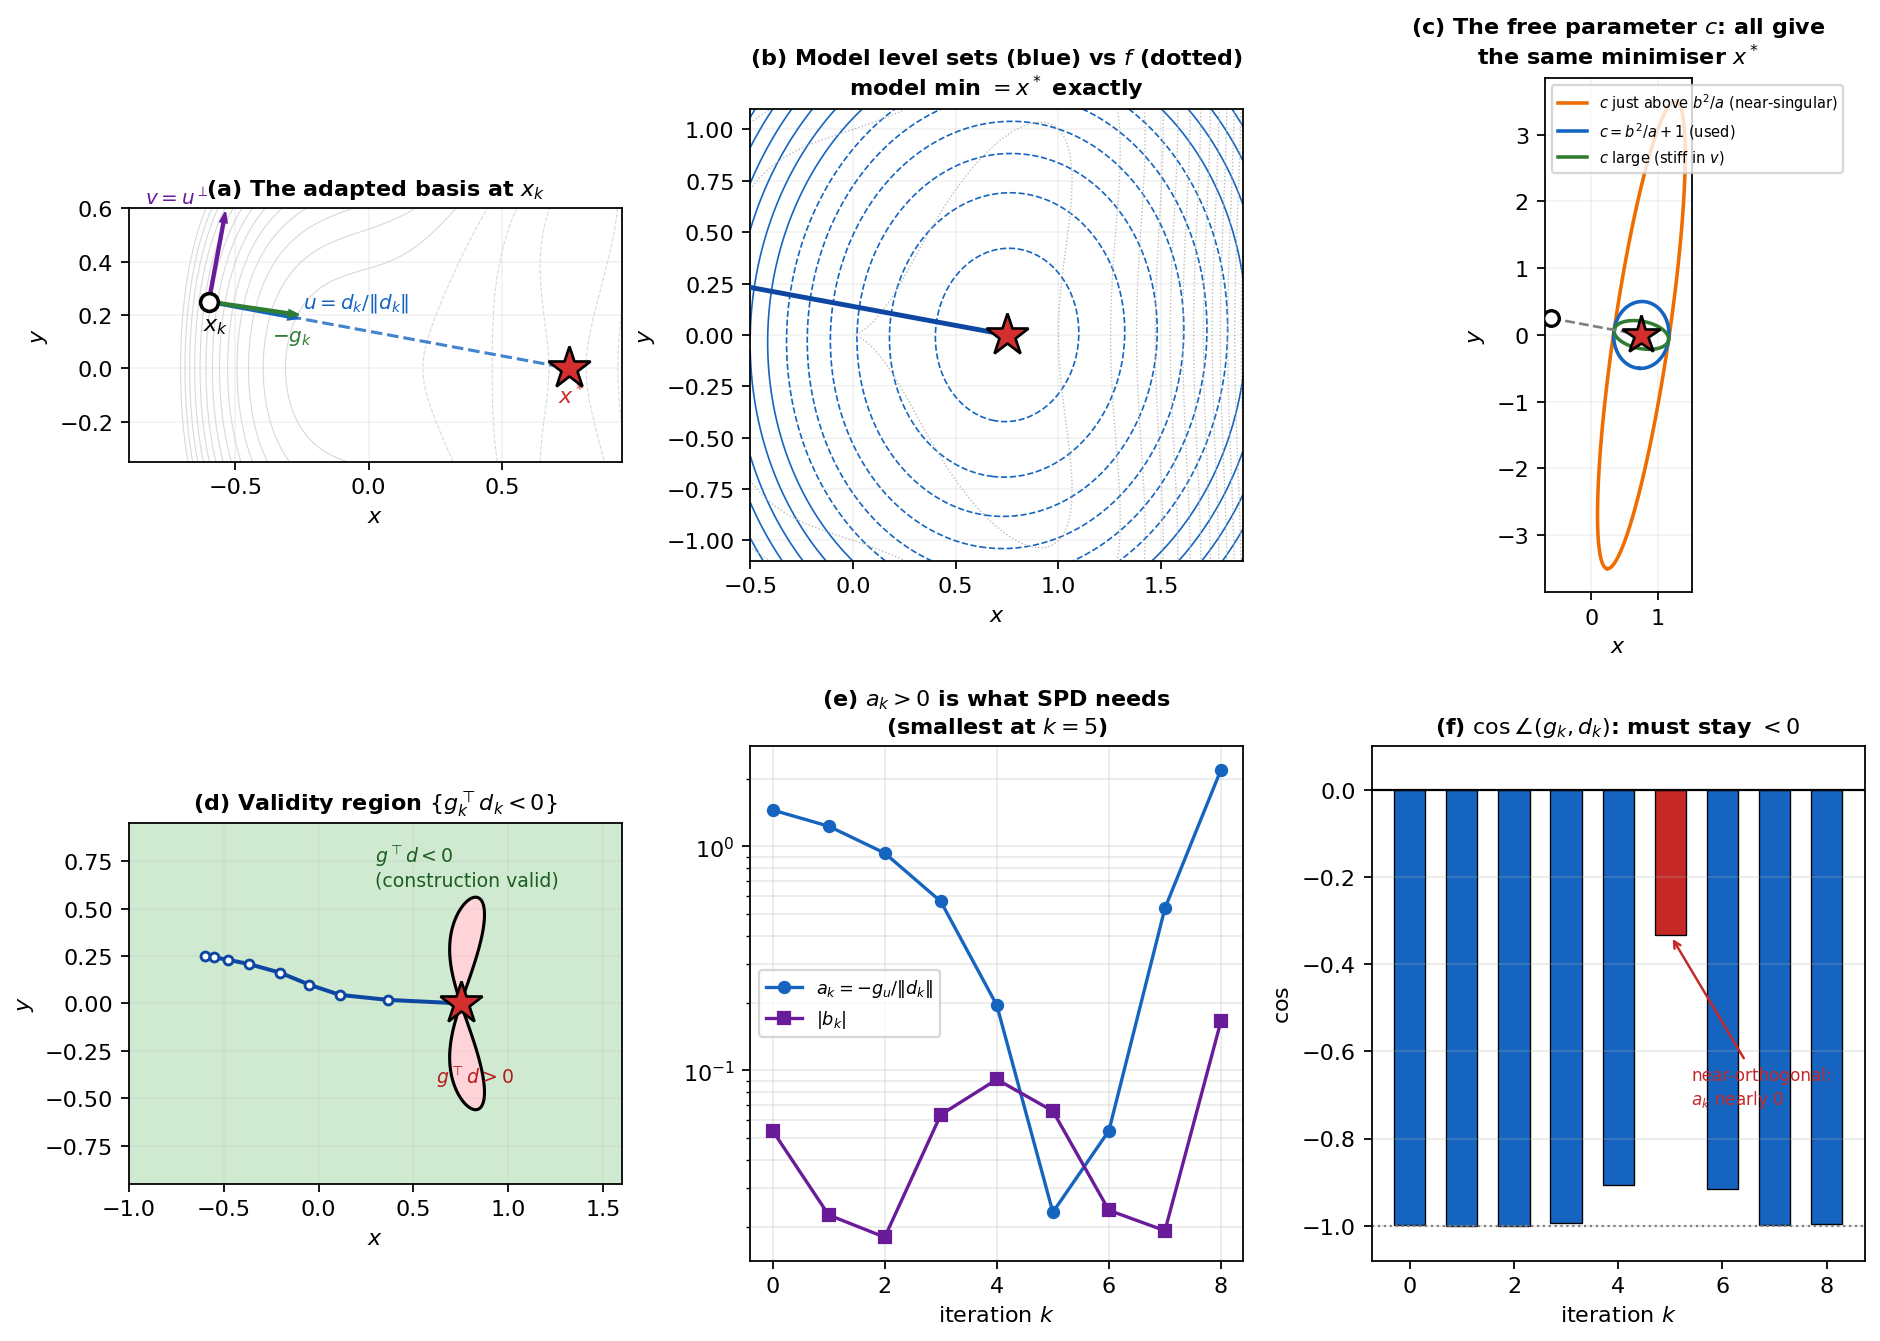
\includegraphics[width=\linewidth]{figs/model_construction.png}
  \caption{The positive definite model of~\eqref{eqn: SPD model} on P1.
    (a) the adapted basis $u = d_k/\norm{d_k}$, $v = u^\perp$ at $x_k$;
    (b) the model level sets, whose minimiser is $x^\star$ exactly;
    (c) the free parameter $c$, every admissible value giving the same minimiser;
    (d) the validity region $\{g_k^\top d_k < 0\}$ of~\eqref{eqn: phi}, the trajectory remaining
    inside it throughout;
    (e) the coefficients $a_k$ and $\abs{b_k}$, positivity of $a_k$ being what positive
    definiteness requires;
    (f) $\cos\angle(g_k,d_k)$, which must stay negative and comes closest to zero at $k=5$, the
    iteration at which the gradient is nearest to orthogonal to the direction of the target.}
  \label{fig: model construction}
\end{figure}

\begin{figure}[htbp]
  \centering
  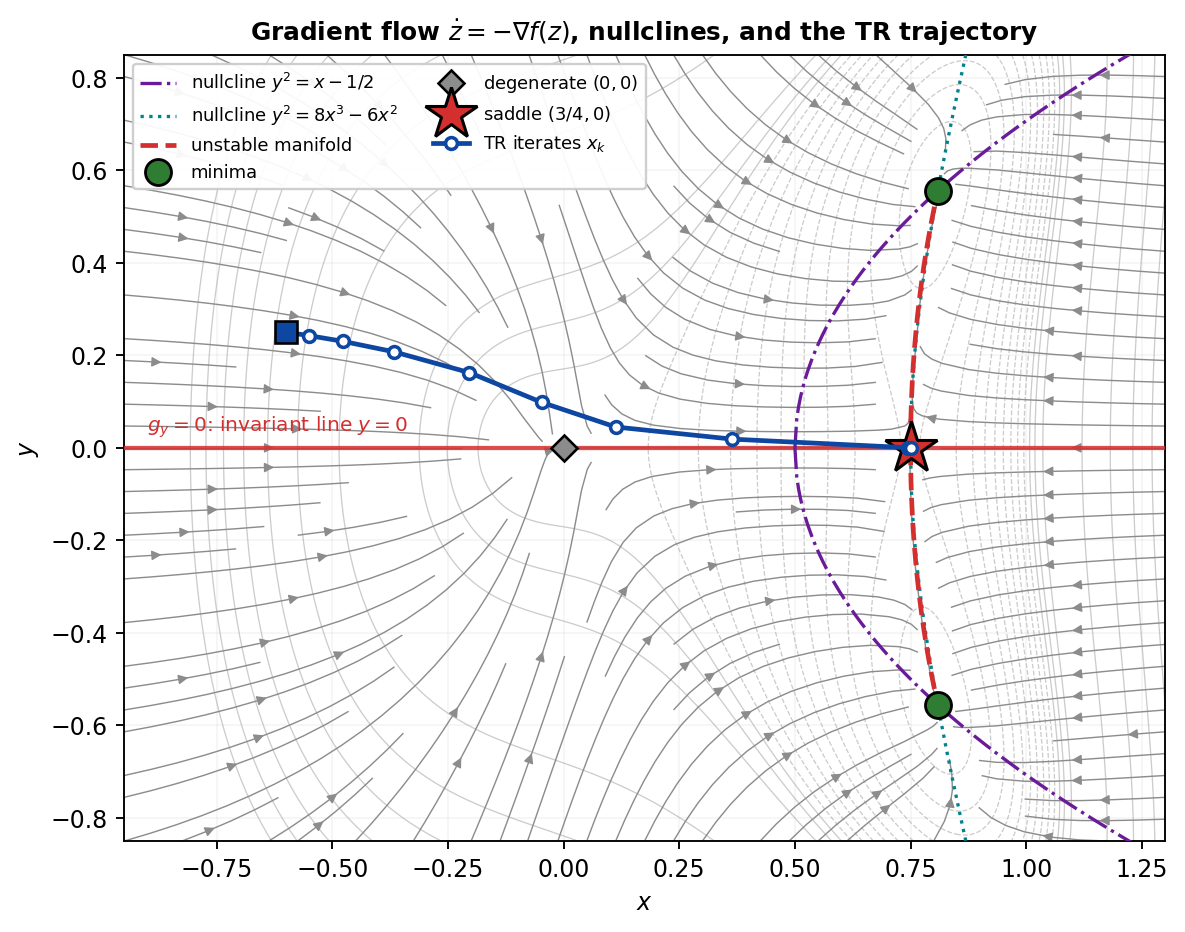
\includegraphics[width=0.72\linewidth]{figs/gradient_flow.png}
  \caption{Gradient flow of P1 with the two nullclines, the invariant line $\{y=0\}$, the
    unstable manifold of the saddle, and the trust-region iterates under the constructed model.
    The iterates start off the stable manifold and are steered onto the saddle, which the flow
    alone would not do.}
  \label{fig: gradient flow}
\end{figure}

\begin{figure}[htbp]
  \centering
  
\includegraphics[width=\linewidth]{figs/diag_spd_saddle.pdf}
  \caption{P1 under the constructed model with $\Rdelta$ and truncated CG.
    (a) the trajectory, ending at the saddle $x^\star = (3/4,0)$;
    (b) the function values, decreasing monotonically to $f(x^\star) = -27/256$ and never
    reaching the minimum value $-1/8$;
    (c) the radius and the step norm, the constraint being active on the shaded iterations;
    (d) the ratio $\rho_k$, which exceeds $\eta_2$ at every iteration but one and exceeds $1$
    from $k=2$ onward. Every first-order diagnostic is healthy throughout.}
  \label{fig: spd saddle run}
\end{figure}

\subsection{P2: a nonsingular saddle with tunable escape rate}
\label{sec: P2}

\begin{equation}
  f_2^{(\varepsilon)}(x,y) = \tfrac12 x^2
    + \varepsilon\Bigl(\tfrac14 y^4 - \tfrac12 y^2\Bigr), \qquad \varepsilon > 0 .
  \label{eqn: P2}
\end{equation}
The origin is a saddle with $\nabla^2 f_2 (0,0)= \operatorname{diag}(1,-\varepsilon)$, hence
$\det = -\varepsilon \neq 0$: \emph{nonsingular} for every $\varepsilon > 0$, with
$\tau(0,0) = \varepsilon > 0$ correctly flagging it. The minimisers are at $(0,\pm 1)$,
at fixed distance from the saddle as $\varepsilon \to 0$, so $\varepsilon$ tunes the escape rate
without collapsing the geometry.

Near the saddle the unstable coordinate obeys $\dot y \approx \varepsilon y$, so
$y(t) \approx y_0 e^{\varepsilon t}$ and the escape time is
\begin{equation}
  k_{\mathrm{esc}} \approx \frac{\ln(1/\abs{y_0})}{\varepsilon},
  \label{eqn: escape}
\end{equation}
linear in $1/\varepsilon$ and only logarithmic in the initial distance to the stable manifold.

\begin{remark}
No nonsingular saddle can have a basin of attraction of positive measure: hyperbolicity forces
the stable set to have dimension equal to the number of positive eigenvalues of
$\nabla^2 f(x^*)$, hence measure zero whenever the saddle is genuine. P2 does not evade this.
What it provides is an \emph{arbitrarily long stall}, which has the same practical consequence:
the method sits within any prescribed tolerance of a nonsingular saddle for as many iterations
as one likes.
\end{remark}

\paragraph{The stall requires a model blind to negative curvature.}
The construction isolates a single ingredient. With the \emph{true} Hessian and a truncated-CG
solver the method escapes in two iterations whatever $\varepsilon$, the model curvature
$-\varepsilon < 0$ being detected on the first CG iteration and the direction of negative
curvature followed to the boundary. The stall appears as soon as the model reports nonnegative
curvature there, which is what BFGS, Gauss--Newton and every positive-definiteness-enforcing
scheme do by construction. With $B_k = \operatorname{diag}(1,c)$ and $c > 0$ fixed, the step along
$y$ is $\abs{s_y} \approx \varepsilon\abs{y}/c$, reproducing~\eqref{eqn: escape} with rate
$\varepsilon/c$. Figure~\ref{fig: slow saddle} confirms the scaling over four decades.

\begin{figure}[htbp]
  \centering
  
\includegraphics[width=\linewidth]{figs/fig12_slow_saddle.pdf}
  \caption{P2 under a model blind to negative curvature.
    (a) the unstable coordinate $\abs{y_k}$ against the iteration count, for four values of
    $\varepsilon$, together with the run under the true Hessian, which escapes in two iterations;
    (b) the measured escape time against $\varepsilon$, matching $\ln(1/\abs{y_0})/\varepsilon$
    over four decades.}
  \label{fig: slow saddle}
\end{figure}

\paragraph{Termination at the saddle.}
The stall becomes an outright failure once $x_k$ has collapsed, since the gradient near the saddle
is $\norm{g_k} \approx \varepsilon\abs{y_k}$. For $\varepsilon = 10^{-4}$ and $y_0 = 10^{-6}$ one
has $\norm{g_0} \approx 10^{-10}$ from the outset, so the method \emph{satisfies its stopping
criterion} at a nonsingular saddle after three iterations. This is a recipe for defeating any
prescribed first-order tolerance $\epsilon_{\mathrm{tol}}$, namely $\varepsilon\abs{y_0} <
\epsilon_{\mathrm{tol}}$. The method does not merely appear to converge. It terminates
successfully and reports a saddle as a solution.

\paragraph{What P1 and P2 separate.}
The two problems distinguish the two ways a first-order guarantee can hold at a point that is not
a minimiser. On P1 the limit is a \emph{degenerate} critical point at which $\tau$ itself
vanishes, so no second-order measure could have flagged it. On P2 the measure $\tau(0,0) =
\varepsilon > 0$ is perfectly informative and never consulted, because what the algorithm sees is
the spectrum of $B_k$ and not that of $\nabla^2 f$. In both the radius mechanism is irrelevant. It
governs how far each step travels, while whether the negative curvature is followed at all is
decided by the model Hessian. This is the empirical form of the claim made throughout Part~II,
that the mechanism decides when a regime is entered and not what the limit is.

\subsection{P3: a family of minimisers with vanishing
         \texorpdfstring{$\lambda^*_{\min}$}{lambda-min}}
\label{sec: P3}

\begin{equation}
  f_3(x,y) = \frac{\sin x}{x} + y^2,
  \qquad \left.\frac{\sin x}{x}\right|_{x=0} \defeq 1 .
  \label{eqn: P3}
\end{equation}
Writing $g(x) = \sin x / x$, the critical points satisfy $\tan x_k = x_k$; the nonzero roots are
$x_k = (k+\tfrac12)\pi - \delta_k$ with $\delta_k \downarrow 0$, one in each interval
$\bigl(k\pi,\ (k+\tfrac12)\pi\bigr)$ for $k \geq 1$. The Hessian is diagonal with eigenvalues
$\{g''(x_k),\,2\}$, and at a critical point the relation $\tan x_k = x_k$ makes two terms of
$g''$ cancel \emph{exactly}:
\begin{equation}
  g''(x_k) = -\frac{\sin x_k}{x_k}.
  \label{eqn: gpp at root}
\end{equation}
Since $\abs{\sin x_k} = \abs{x_k}/\sqrt{1+x_k^2} \to 1$, we have
$\abs{g''(x_k)} \sim 1/\abs{x_k}$, alternating in sign. Along the subsequence with
$g''(x_k) > 0$ the critical points are minimisers with $\lambda^*_{\min} \to 0$, so by
\eqref{eqn: kappa} the constant $\overline{\kappa} = 8/\lambda^*_{\min}$ can be made arbitrarily
large by choosing a minimiser far from the origin. P3 is therefore the natural vehicle for
testing Claims~\ref{claim: zeta} and~\ref{claim: mu}. Table~\ref{tab: P3 kappa} gives the first
few values.

\begin{table}[htbp]
  \centering
  \caption{Minimisers of $f_3$ of~\eqref{eqn: P3} and the associated constant
           $\overline{\kappa} = 8/\lambda^*_{\min}$. Only the critical points with
           $g''(x^*) > 0$ are minimisers in $x$; the interleaving points are saddles.}
  \label{tab: P3 kappa}
  \small
  \begin{tabular}{rrrrl}
    \toprule
    $x^*$ & $g''(x^*)$ & $\lambda^*_{\min}$ & $\overline{\kappa} = 8/\lambda^*_{\min}$ & Type \\
    \midrule
    $4.4934$  & $+0.21723$ & $0.21723$ & $36.83$ & minimiser \\
    $7.7253$  & $-0.12837$ & ---       & ---     & saddle \\
    $10.9041$ & $+0.09133$ & $0.09133$ & $87.60$ & minimiser \\
    $14.0662$ & $-0.07091$ & ---       & ---     & saddle \\
    $17.2208$ & $+0.05797$ & $0.05797$ & $138.00$ & minimiser \\
    \bottomrule
  \end{tabular}
\end{table}

\subsection{P4: a set of thirty classical problems}
\label{sec: analytic set}

The three problems above are diagnostic instruments: each isolates one pathology. For the
aggregate questions---which value of a parameter to choose, which mechanism to prefer---we use a
set of thirty small unconstrained problems drawn from the classical literature, listed in
Table~\ref{tab: analytic set}. They are deliberately unexceptional: smooth, low-dimensional,
mostly with a unique attracting minimiser in the basin of the standard starting point, and
covering the usual difficulties (narrow valleys, ill-conditioning, quartic flatness, exponential
and trigonometric terms). Derivatives are exact.

Thirty problems is too few to support a claim about typical behaviour in general, and we do not
make one; the set exists to give the parameter sweeps of Section~\ref{sec: exp zeta} and
Section~\ref{sec: exp mu} an aggregate reading, and to establish the reporting format that
Experiment~\ref{exp: cutest} will apply at scale.

\begin{table}[htbp]
  \centering
  \caption{The thirty-problem analytic set P4. Dimension $n$ and the standard starting point are
           those of the source; where a problem appears twice it is with a different $x_0$.}
  \label{tab: analytic set}
  \scriptsize
  \begin{tabular}{llllllll}
    \toprule
    Problem & $n$ & Problem & $n$ & Problem & $n$ & Problem & $n$ \\
    \midrule
    ROSENBR    & 2 & CAMEL3    & 2 & LOGQUAD   & 2 & SQRTSUM   & 2 \\
    ROSENBR2   & 2 & CAMEL6    & 2 & QUARTIC2  & 2 & ILLCOND   & 2 \\
    BEALE      & 2 & TRID2     & 2 & QUARTSUM  & 2 & EXTROSEN3 & 3 \\
    POWELLSG   & 4 & DIXONPR2  & 2 & TRIGQUAD  & 2 & TRID3     & 3 \\
    WOOD       & 4 & ZAKHAROV2 & 2 & CUBEROOT  & 2 & EXPSUM3   & 3 \\
    HIMMELBLAU & 2 & EXPFIT2   & 2 & QUART4    & 2 & PROD3     & 3 \\
    BOOTH      & 2 & ROSENPERT & 2 & EXPQUAD   & 2 & QUART4V   & 4 \\
    MATYAS     & 2 &           &   & PARAB     & 2 &           &   \\
    \bottomrule
  \end{tabular}
\end{table}

%=======================================================================
\section{Results}
\label{sec: results}
\label{sec: experiments}
%=======================================================================

Numbers marked \provisional{} are from the preliminary campaign over three
two-variable problems and are reported here for the shape of the table rather
than for their values. Runs of that length settle no asymptotic question, and the
widened campaign replaces every one of them.


\subsection{The radius regimes}
\label{sec: res asymptotics}

\PartII{} predicts three regimes: $\sum_k \Delta_k^2/M_k < \infty$ for the
criticality-anchored rules under no hypothesis on the iterates,
$\sum_k \Delta_k < \infty$ for the step-driven rules in the local regime, and
$\liminf_k \Delta_k > 0$ for the fixed-factor rules.

Table~\ref{tab: sums} reports the three series per run. The separation between
$\Rdelta$ and the criticality-anchored rules is unambiguous: the radius of the
former grows geometrically, and both of its series diverge to the point of
overflowing double precision, which is an overflow rather than a proof. The
criticality-anchored rules give small partial sums in every column.

\begin{table}[htbp]
  \centering
  \caption{The three radius series on P1 from $x_0 = (-0.5,0.6)$, exact Hessian,
           truncated conjugate gradient, four hundred iterations.\provisional{}
           $M_k = \max_{i\leq k}\norm{H_i}$, that is $L = 0$: the Lipschitz
           constant is not known, and omitting it changes the constant rather
           than the convergence. These are partial sums over a finite run and
           settle nothing on their own.}
  \label{tab: sums}
  \small
  \begin{tabular}{@{}lrrr@{}}
    \toprule
    Mechanism & $\sum_k\Delta_k$ & $\sum_k\Delta_k^2$ & $\sum_k\Delta_k^2/M_k$ \\
    \midrule
    $\Rdelta$                     & $2.6\times10^{120}$ & overflow & \provisional \\
    $\Rstep$                      & $7.98\times10^{2}$  & $1.60\times10^{3}$ & \provisional \\
    $\Rdfo$ ($\zeta = 1$)         & $8.28\times10^{0}$  & $1.22\times10^{0}$ & \provisional \\
    $\Rgrad$ (capped)             & $6.48\times10^{0}$  & $4.28\times10^{-1}$ & \provisional \\
    $\Rgrad$ (uncapped)           & $2.77\times10^{2}$  & $1.92\times10^{2}$ & \provisional \\
    \bottomrule
  \end{tabular}
\end{table}

Two rows require comment, and both are consistent with \PartII{} rather than
contrary to it. The step-driven rule shows no sign of the summability
$\sum_k\Delta_k < \infty$, and it is not predicted to: this run converges to the
degenerate origin of P1, where $\nabla^2 f_1$ is singular, so the local
hypothesis under which that summability is proved does not hold. The uncapped
gradient-scaled rule likewise shows large partial sums, and \PartII{} is explicit
that its asymptotic conclusions are unavailable once the multiplier diverges. A
run outside the hypotheses of a proposition is not evidence against it, and the
table is reported at a nondegenerate minimiser as well.

\begin{remark}
The third column is not a refinement of the second. The two agree up to a
constant only while $\{\norm{H_k}\}$ is bounded, which is the hypothesis the
$M_k$ form exists to drop, so they separate exactly on the runs where the model
curvature grows.
\end{remark}


\subsection{Eventual inactivity}
\label{sec: res inactivity}

The observable is $k_\star$, and its absence. Table~\ref{tab: inactivity v4}
reports it beside the tail-active fraction and the number of runs whose
constraint bound to the last iteration.

\begin{table}[htbp]
  \centering
  \caption{Inactivity by mechanism.\provisional{} \emph{measured} counts runs long
           enough for a tail fraction to carry information; \emph{never} counts
           runs whose constraint never stopped binding, which for a rule below
           its threshold is the finding rather than a missing entry.}
  \label{tab: inactivity v4}
  \small
  \begin{tabular}{@{}lrrrr@{}}
    \toprule
    Mechanism & runs & solved & mean tail active & never \\
    \midrule
    $\Rdelta$                       & 3 & 3 & $0.000$ & 0 \\
    $\Rstep$                        & 3 & 3 & $0.611$ & \provisional \\
    $\Rdfo$ ($\zeta = 1$)           & 3 & 3 & $0.000$ & 0 \\
    $\Rdfo$ ($\zeta = 0.01$)        & 3 & 3 & $0.389$ & \provisional \\
    $\Rgrad$                        & 3 & 3 & $0.222$ & \provisional \\
    $\Rgrad$ ($\overline{\mu}=0.05$)& 3 & 3 & $1.000$ & 3 \\
    \bottomrule
  \end{tabular}
\end{table}

The capped gradient-scaled rule with a parameter far below its threshold binds on
every late iteration, as predicted. The remaining entries are not yet evidence
either way: the runs are between nine and forty-eight iterations long, so the
last tenth is one to five iterations and the fraction is quantised. The three
intermediate values in the table are the resolution of the statistic and not a
property of the mechanisms, which is why they are reported with the run count
beside them and why the widened campaign is required before any of them is read.

A first-order convergence test does not separate these configurations: every one
of them drives $\norm{g_k}$ monotonically to zero. That is the practical content
of the claim, and it is what makes the activity flag worth recording.


\subsection{Inactivity of the trust region}
\label{sec: exp inactivity}

\begin{experiment}[Direct measurement of inactivity]
\label{exp: inactivity}
For each run, record the indicator $\mathbb{1}\{\norm{s_k} = \Delta_k\}$ and report the fraction
of active iterations over the last decile of the run. Report also $\sum_k \Delta_k$ and
$\sum_k \Delta_k^2$ to test Claim~\ref{claim: asymptotics}.
\end{experiment}

\subsection{The thresholds}
\label{sec: res thresholds}

On P3 the minimiser at $x^* \approx (10.904, 0)$ has
$\lambda^*_{\min} = 0.09133$, and the three thresholds \PartII{} names are
separated by more than an order of magnitude:

\begin{equation}
  \underbrace{\frac{1-\gamma_2}{\lambda^*_{\min}(\gamma_3+1-\gamma_2)} = 2.19}_{\text{$\Rdfo$ trapped below}}
  \qquad
  \underbrace{\frac{1}{\lambda^*_{\min}} = 10.95}_{\text{exact}}
  \qquad
  \underbrace{\kbar = \frac{8}{\lambda^*_{\min}} = 87.60}_{\text{sufficient}} .
  \label{eqn: three thresholds}
\end{equation}

The sufficient condition of the inactivity theorem overshoots the exact threshold
by a factor of eight, of which four is intrinsic to the step bound and two is the
price of a neighbourhood bound in place of the eigenvalue. On the sinc family
$\kbar = 8\sqrt{1+y_j^2}$ at the $j$-th minimiser, so it is unbounded over the
minimisers of one fixed $C^\infty$ function with bounded Hessian, and no finite
parameter is above it everywhere.

\begin{table}[htbp]
  \centering
  \caption{Behaviour on P3 near $x^* \approx (10.904,0)$, from
           $x_0 = (9.6,0.4)$ with $\Delta_0 = 0.03$, exact Hessian, truncated
           conjugate gradient, budget four thousand
           iterations.\provisional{} Thresholds
           as in~\eqref{eqn: three thresholds}. \emph{Active} counts iterations
           on which $\norm{s_k} = \Delta_k$.}
  \label{tab: kappa}
  \small
  \begin{tabular}{@{}llrrll@{}}
    \toprule
    Mechanism & Parameter & Iters & Active & Dist.\ to $x^*$ & Status \\
    \midrule
    $\Rdfo$  & $\zeta = 60$, above exact       & $9$    & $5$    & $1.8\times10^{-15}$ & converged \\
    $\Rdfo$  & $\zeta = 0.5$, below trapping   & $4000$ & $4000$ & $6.0\times10^{-8}$  & budget \\
    $\Rgrad$ & $\overline{\mu} = 50$           & $6$    & $1$    & $1.8\times10^{-15}$ & converged \\
    $\Rgrad$ & $\overline{\mu} = 1$            & $4000$ & $4000$ & $4.0\times10^{-8}$  & budget \\
    $\Rgrad$ & uncapped, $\mu_0 = 0.1$         & $55$   & $53$   & $7.1\times10^{-15}$ & converged \\
    $\Rstep$ & ---                             & $9$    & $5$    & $1.8\times10^{-15}$ & converged \\
    $\Rdelta$& ---                             & $9$    & $5$    & $1.8\times10^{-15}$ & converged \\
    \bottomrule
  \end{tabular}
\end{table}

The split is complete and binary. Every configuration whose parameter sits above
the exact threshold reaches inactivity within a few iterations; the two that sit
below the trapping threshold bind on all four thousand. Both groups drive
$\norm{g_k}$ towards zero, and the failing runs reach $10^{-8}$ in distance, so
nothing short of the activity flag distinguishes them.

Neither observation resolves where the transition lies. The data bracket it
between $\zeta = 0.5$ and $\zeta = 60$, which contains the exact threshold
$10.95$ and excludes neither it nor a value some way from it; a sweep at
$\zeta \in \{2, 4, 8, 11, 16, 32\}$ is what closes the interval, and is the
measurement that quantifies the factor of eight. The sufficient condition
$\zeta > \kbar = 87.60$ is met by none of these runs, and inactivity is
nonetheless reached from $\zeta = 60$: the condition is sufficient and not
necessary, and how far from necessary is the question the sweep answers.

The uncapped rule is the theoretically distinguished case, and it behaves as
\PartII{} requires. Started at $\mu_0 = 0.1$, three orders of magnitude below
$\kbar$ and below the exact threshold, it converges without a cap to reach: the
multiplier climbs geometrically on very successful iterations until the region
stops binding. It is the only rule in the survey whose inactivity depends on no
parameter the user cannot check, and the fifty-three active iterations before it
succeeds are the cost of the climb.

\begin{remark}
The climb is bounded. \PartII{} places the multiplier's window between
$D = 2(1-\xi)/\kumh$ and $C = (2/m)(1+\sqrt{M/m})$, with $\kbar$ inside it, so
the number of expansions after the iterates settle is at most
$\log_{\gamma_3}(\gamma_3 C/\mu_0)$. Counting expansion branches against that
bound is a direct test of the window, and is reported in
Section~\ref{sec: res interaction}.\provisional
\end{remark}


\subsection{Influence of the criticality parameter \texorpdfstring{$\zeta$}{zeta}}
\label{sec: exp zeta}

\begin{experiment}[Influence of the criticality parameter]
\label{exp: zeta}
On P3, target the minimiser $x^* \approx (10.904,\,0)$ with
$\overline{\kappa} = 43.80$. Start from $x_0 = (9.6,\,0.4)$ with $\Delta_0 = 0.03$ and sweep
$\zeta$ across $\overline{\kappa}$. Record the number of iterations, the number of iterations on
which the trust-region constraint is active, and the distance to $x^*$.
\end{experiment}

\begin{experiment}[$\zeta$ sweep across models, on P1]
\label{exp: zeta P1}
Sweep $\zeta \in \{0.001, 0.01, 0.1, 0.5, 1, 2, 10, 100\}$ on P1 from $x_0 = (-0.5, 0.6)$ for
each of the three model Hessians.
\end{experiment}

Table~\ref{tab: zeta P1} shows a phenomenon worth recording: with the true Hessian, $\zeta$
\emph{saturates}. All values $\zeta \geq 0.5$ produce bit-identical trajectories, because the
shrink branch, although it still fires, never reduces the radius enough to alter the step the
solver returns. With quasi-Newton models the saturation point moves out by two orders of
magnitude and the parameter continues to matter over the whole range. A $\zeta$-sweep therefore
measures something quite different depending on the model, which is a caution against reporting
a single recommended value.

\subsubsection*{Aggregate view: which $\zeta$ should one choose?}

The two preceding tables show what $\zeta$ does on individual problems. To ask which value one
should actually pick, we need an aggregate over a heterogeneous set, and a performance profile is
the appropriate instrument. Figure~\ref{fig: profile zeta} reports the sweep over the analytic
set of Section~\ref{sec: analytic set}.

The shape of the answer is more informative than any single recommended value. Efficiency---the
intercept $\pi_s(1)$---is essentially flat for $\zeta \geq 0.1$, varying between $0.67$ and
$0.73$ with no trend. What separates the values is \emph{reliability}: $\zeta = 0.01$ solves only
$18$ of $30$ problems, $\zeta = 0.1$ solves $28$, and every $\zeta \geq 2$ solves all $30$
(Table~\ref{tab: zeta reliability}). A small $\zeta$ does not make the method slower on the
problems it solves; it makes it fail outright on problems where the threshold of
Claim~\ref{claim: zeta} is not met within the budget.

This is exactly the signature Part~II predicts. Below the problem-dependent threshold
$\overline{\kappa} = 8/\lambda^*_{\min}$ the trust-region constraint never stops binding, and the
method converges at best linearly; whether it finishes within a fixed budget then depends on how
far below the threshold $\zeta$ sits. Since $\overline{\kappa}$ varies across the test set---it is
a property of each problem's solution---no single $\zeta$ is above threshold everywhere, and the
reliability curve is the empirical distribution of that mismatch.

The practical reading is that $\zeta$ should be chosen \emph{generously}. The cost of an
over-large $\zeta$ is nil on this set: $\zeta = 100$ is indistinguishable from $\zeta = 2$ on both
measures, because once the constraint is inactive the rule no longer influences the step. The
cost of an over-small $\zeta$ is a $40\%$ failure rate. Asymmetric risk of this kind argues
against the instinct to keep a trust-region parameter conservative.

\begin{table}[htbp]
  \centering
  \caption{Reliability and efficiency of $\Rdfo$ as a function of $\zeta$ on the $30$-problem
           analytic set, exact Hessian, truncated CG, $\epsilon_g = 10^{-6}$, budget $1000$
           iterations. Median iteration count is over solved problems only. Efficiency is flat;
           reliability is not.}
  \label{tab: zeta reliability}
  \small
  \begin{tabular}{rrrr}
    \toprule
    $\zeta$ & Solved & Median iters & $\pi_s(1)$ \\
    \midrule
    $0.01$  & $18/30$ & $8.0$ & $0.267$ \\
    $0.1$   & $28/30$ & $7.5$ & $0.733$ \\
    $0.5$   & $29/30$ & $6.0$ & $0.667$ \\
    $1$     & $29/30$ & $6.0$ & $0.733$ \\
    $2$     & $30/30$ & $6.5$ & $0.700$ \\
    $10$    & $30/30$ & $5.5$ & $0.700$ \\
    $100$   & $30/30$ & $5.5$ & $0.733$ \\
    \bottomrule
  \end{tabular}
\end{table}

\begin{figure}[htbp]
  \centering
  \begin{tikzpicture}
    \begin{axis}[
        width=0.70\textwidth, height=6.6cm,
        xlabel={$\tau$ (performance ratio, iteration count)},
        ylabel={$\pi_s(\tau)$},
        xmode=log, xmin=1, xmax=250, ymin=0, ymax=1.02,
        legend pos=south east, legend style={font=\scriptsize, fill opacity=0.9,
                                             text opacity=1},
        legend columns=2,
        grid=both, grid style={gray!22},
        every axis plot/.append style={line width=0.9pt},
      ]
      \input{prof_zeta.tex}
    \end{axis}
  \end{tikzpicture}
  \caption{Performance profiles of $\Rdfo$ as a function of $\zeta$ on the analytic set. The
    curves are nearly indistinguishable in their left-hand behaviour---$\zeta$ barely affects
    efficiency---but separate cleanly in their right-hand asymptotes, which are the reliability
    figures of Table~\ref{tab: zeta reliability}. Choosing $\zeta$ too small costs solved
    problems, not iterations; choosing it too large costs nothing on this set.}
  \label{fig: profile zeta}
\end{figure}

\begin{table}[htbp]
  \centering
  \caption{$\zeta$ sweep on P1 from $x_0 = (-0.5,0.6)$, truncated CG, budget $4000$.
           Iteration counts; ``---'' marks a run that exhausted the budget. With the true
           Hessian all runs with $\zeta \geq 0.5$ have identical iterate sequences.}
  \label{tab: zeta P1}
  \small
  \begin{tabular}{rrrr}
    \toprule
    $\zeta$ & True Hessian & SR1 & L-BFGS($5$) \\
    \midrule
    $0.001$ & ---   & ---   & ---   \\
    $0.01$  & ---   & ---   & ---   \\
    $0.1$   & $15$  & ---   & ---   \\
    $0.5$   & $15$  & ---   & ---   \\
    $1$     & $15$  & ---   & ---   \\
    $2$     & $15$  & $2675$ & $1051$ \\
    $10$    & $15$  & $290$  & $24$   \\
    $100$   & $15$  & $21$   & $24$   \\
    \bottomrule
  \end{tabular}
\end{table}

\subsection{Influence of the cap \texorpdfstring{$\overline{\mu}$}{mu-bar}}
\label{sec: exp mu}

\begin{experiment}[The cap and the threshold]
\label{exp: mu}
On P1 from $x_0 = (-0.5,0.6)$, sweep
\begin{equation*}
  \overline{\mu} \in \{0.01,\ 0.05,\ 0.1,\ 0.3,\ 0.5,\ 1,\ 2,\ 4,\ 8,\ 128\}
\end{equation*}
for each model Hessian and each subproblem solver, and classify the limit point.
\end{experiment}

This is the sharpest result of the analytic campaign, and it is stronger than Part~II predicts.
With the true Hessian, $\overline{\mu}$ affects only the speed: every value drives the iterates
to the degenerate origin, taking $41$ iterations at $\overline{\mu} = 128$ and exceeding the
budget at $\overline{\mu} \leq 1$. With a quasi-Newton model there is a
\emph{threshold near $\overline{\mu} \approx 0.5$ that changes the destination}
(Table~\ref{tab: mu threshold}). Below it, the accumulated curvature is never used and the run
crawls to the degenerate origin, where $\lambda_{\min}(\nabla^2 f_1) = 0$ and the limit is not a
minimiser. Above it, the curvature enters the step and the run reaches a genuine local minimiser
with $\lambda_{\min}(\nabla^2 f_1) = 0.4947$, in fewer than thirty iterations.

The cap that the asymptotic theory requires therefore carries a cost that is not merely a
constant factor in the rate: chosen too small, it changes which critical point is reached, and
converts a second-order-adequate limit into one that fails second-order optimality. The
mechanism behind the threshold is Claim~\ref{claim: cauchy}, examined in
Experiment~\ref{exp: interaction}.

\begin{table}[htbp]
  \centering
  \caption{The $\overline{\mu}$ threshold for $\Rgrad$ with quasi-Newton models on P1,
           $x_0 = (-0.5, 0.6)$, budget $30\,000$. Below $\overline{\mu} \approx 0.5$ the limit
           is the degenerate origin, which is not a minimiser; above it the run reaches a local
           minimiser. Both solvers and both models agree on the threshold.}
  \label{tab: mu threshold}
  \small
  \begin{tabular}{llrlrl}
    \toprule
    Model & $\overline{\mu}$ & Solver & Status & Iters & Limit \\
    \midrule
    \multirow{5}{*}{L-BFGS($5$)}
      & $0.10$ & CG    & budget    & $30\,000$ & origin (degenerate) \\
      & $0.30$ & CG    & budget    & $30\,000$ & origin (degenerate) \\
      & $0.50$ & CG    & stagnated & $85$      & $\text{min}^{+}$ \\
      & $1.00$ & CG    & stagnated & $27$      & $\text{min}^{-}$ \\
      & $2.00$ & CG    & converged & $15$      & $\text{min}^{-}$ \\
    \midrule
    \multirow{5}{*}{SR1}
      & $0.10$ & CG    & budget    & $30\,000$ & origin (degenerate) \\
      & $0.30$ & CG    & budget    & $30\,000$ & origin (degenerate) \\
      & $0.50$ & CG    & stagnated & $85$      & $\text{min}^{+}$ \\
      & $1.00$ & CG    & converged & $15$      & $\text{min}^{-}$ \\
      & $2.00$ & exact & converged & $13$      & $\text{min}^{-}$ \\
    \bottomrule
  \end{tabular}
\end{table}

Table~\ref{tab: kappa} also records the unbounded $\Rgrad$ variant, which is the theoretically
interesting case. Started at $\mu_0 = 0.1 \ll \overline{\kappa}$ it nevertheless converges, in
$55$ iterations: with no cap, $\mu_k$ grows geometrically on very successful iterations until
the trust-region constraint stops binding. This is the empirical counterpart of the unconditional
statement in Part~II, and it is the strongest practical argument for the unbounded variant---it
recovers from a parameter choice that traps the capped rule permanently.

\subsection{The rate after inactivity}
\label{sec: res rate}

This is the sharpest claim of \PartII: conditional on the region becoming
inactive, the observed order is that of the underlying quasi-Newton iteration and
does not depend on the mechanism, which decides only when that regime is entered.

The estimate is a regression of $\log\norm{g_{k+1}}$ on $\log\norm{g_k}$ over
accepted iterations beyond $k_\star$. Conditioning is necessary and not
sufficient: a tail of four points returns a number that looks like a rate and is
not one, so runs with fewer than six inactive iterations are counted and excluded
rather than reported.

\begin{table}[htbp]
  \centering
  \caption{Observed order by problem and mechanism, exact Hessian.\provisional{}
           Entries are the estimate on the inactive tail; \emph{short} marks a
           tail too brief to fit.}
  \label{tab: order v4}
  \small
  \begin{tabular}{@{}lrrrrr@{}}
    \toprule
    Problem & $\Rdelta$ & $\Rstep$ & $\Rdfo$ & $\Rgrad$ & $\Rgrad(\overline{\mu})$ \\
    \midrule
    AKIVA    & $1.415$ & short   & $1.415$ & $1.415$ & $1.415$ \\
    BEALE    & $1.712$ & $1.445$ & $1.445$ & $2.003$ & $2.003$ \\
    BOXBODLS & $1.462$ & short   & $1.444$ & short   & short   \\
    \bottomrule
  \end{tabular}
\end{table}

The first row is the claim in miniature: five mechanisms, one problem, the same
estimate to three decimal places. The second row splits, and the reason is
visible in $k_\star$ rather than in the rate. The gradient-scaled rules reach
inactivity at $k_\star = 10$ of eighteen iterations and the others at
$k_\star = 2$ of nine, so the two groups fit over different phases of runs of
different lengths, and the difference between $1.445$ and $2.003$ measures how
much pre-asymptotic behaviour each tail still contains.

The table therefore neither confirms nor refutes the claim, and the reason is a
property of the problem set rather than of the mechanisms: a nine-iteration run
to machine precision has no asymptotic phase to speak of. What the claim requires
is problems with long local phases, which is what the widened campaign supplies,
and the design point is that the order be compared only within a problem and only
across mechanisms that reached inactivity with comparable tails.\provisional

\begin{remark}
An order estimate is about the mechanism only if the model was consistent. The
recorded $\gamma_k$ and $\xi_k$ decide that, and a run whose Dennis--Mor\'e
residual has not fallen has no asymptotic rate to attribute to anything. Both are
reported with the order.
\end{remark}


\subsection{Influence of the mechanism on the rate of convergence}
\label{sec: exp rate}

\begin{experiment}[Observed local rate]
\label{exp: rate}
On problems where the limit is a nondegenerate minimiser, estimate the local rate by regressing
$\log\norm{g_{k+1}}$ on $\log\norm{g_k}$ over the last $20$ successful iterations, and report
the estimated order together with the iteration at which the trust region last binds.
\end{experiment}
\begin{table}[htbp]
  \centering
  \caption{Sublinear approach to the degenerate origin of P1 under $\Rgrad$ with
           $\overline{\mu} = 0.05$ and truncated CG. The product $k\norm{x_k}$ settles to a
           constant, so $\norm{x_k} = \Theta(1/k)$.}
  \label{tab: crawl}
  \small
  \begin{tabular}{rrrr}
    \toprule
    $k$ & $\norm{g_k}$ & $\norm{x_k}$ & $k\,\norm{x_k}$ \\
    \midrule
    $10$      & $3.61\times10^{-1}$ & $4.05\times10^{-1}$ & $4.049$ \\
    $100$     & $1.36\times10^{-2}$ & $4.69\times10^{-2}$ & $4.692$ \\
    $1\,000$  & $1.15\times10^{-4}$ & $6.16\times10^{-3}$ & $6.159$ \\
    $5\,000$  & $5.14\times10^{-6}$ & $1.31\times10^{-3}$ & $6.539$ \\
    $20\,000$ & $3.30\times10^{-7}$ & $3.31\times10^{-4}$ & $6.630$ \\
    \bottomrule
  \end{tabular}
\end{table}

\subsection{Second order: the criticality measure at a saddle}
\label{sec: res second order}

Under $\norm{g_k}$ as the criticality measure, a criticality-anchored radius
collapses at a saddle: $\Rgrad(\norm{g})$ halts outright where the gradient
vanishes, and $\Rdfo(\norm{g})$ contracts geometrically. Replacing the measure by
$\tau_k = \max\{\norm{g_k}, -\lambda_k^-\}$ repairs both, since
$-\lambda_k^-$ stays bounded away from zero at a saddle the model can see.

Each $\norm{g}$-anchored rule is run beside its $\tau$-anchored twin on the
saddle problems, under both subproblem solvers, and the outcome is read from
three quantities: the radius trajectory, which collapses in one case and does not
in the other; the certified second-order status; and the limit reached. The
distinction the certification makes is worth stating, because it is easy to lose:
the status certifies $\lambda_{\min}(H_k) \geq -\varepsilon_H$, a statement about
the model, and a configuration that solves every problem while certifying none
has been running a first-order method under a second-order name.\provisional

The measure is half of the requirement and the solver is the other half. The
$\tau$ anchoring keeps the radius away from zero at the saddle, and a step that
exploits negative curvature is what converts that radius into escape. A truncated
conjugate-gradient solver supplies such a step only when the Krylov space it
generates meets the negative-curvature subspace, and the configuration in which
it does not is realisable rather than hypothetical: with $g_k$ in the
positive-curvature eigenspace the first direction is $-g_k$, the curvature along
it is positive, the residual vanishes, and the iteration terminates at an
interior point while $\lambda_k^- < 0$. The eigenpoint construction supplies the
step the assumption asks for.


\subsection{Mechanism against model}
\label{sec: res interaction}

The mechanism and the model have different jobs, and the interaction between them
is where a parameter chosen for one reason has consequences of another kind.

With a truncated conjugate-gradient solver and a cap small enough that the first
conjugate-gradient iterate leaves the region, the returned step is the Cauchy
point: the alignment $\cos(s_k,-g_k)$ is one to machine precision, the inner
iteration count is one, and the model Hessian has influenced nothing but the
acceptance test. The method has become gradient descent with step length
$\overline{\mu}\norm{g_k}$, and it inherits gradient-descent behaviour, including
its limit.

\begin{table}[htbp]
  \centering
  \caption{Truncated conjugate gradient under $\Rgrad$ on P1, exact
           Hessian.\provisional{} For $\overline{\mu} \leq 0.1$ the solver
           truncates on its first iteration and returns the Cauchy point.}
  \label{tab: cauchy}
  \small
  \begin{tabular}{@{}rrll@{}}
    \toprule
    $\overline{\mu}$ & CG iters & active & $\cos(s_k,-g_k)$ \\
    \midrule
    $0.01$ & $1$ & yes & $1.00000000000000$ \\
    $0.05$ & $1$ & yes & $1.00000000000000$ \\
    $0.10$ & $1$ & yes & $1.00000000000000$ \\
    $0.30$ & $2$ & no  & $0.87728513992144$ \\
    $1.00$ & $2$ & no  & $0.87728513992144$ \\
    \bottomrule
  \end{tabular}
\end{table}

The consequence is not a constant factor. On P1 with a quasi-Newton model there
is a threshold near $\overline{\mu} \approx 0.5$ below which the accumulated
curvature never enters the step and the run crawls to the degenerate origin,
where $\lambda_{\min}(\nabla^2 f_1) = 0$ and the limit is not a minimiser, and
above which the run reaches a genuine local minimiser in fewer than thirty
iterations.\provisional{} A cap chosen conservatively, to satisfy the
boundedness hypothesis the asymptotic theory of \PartII{} requires, can therefore
change which critical point is reached.

No first-order diagnostic reveals this. The ratio is healthy, the gradient norm
decreases monotonically, and the radius behaves exactly as the rule prescribes.
The only symptom is slowness, and slowness is easy to attribute to the problem.
The inner-iteration count and the alignment are what name it, which is the
practical reason for recording them.


\subsection{Interaction between mechanism and Hessian approximation}
\label{sec: exp interaction}

\begin{experiment}[The Cauchy-point degeneration]
\label{exp: interaction}
With truncated CG and $\Rgrad$, record for each iteration the number of CG iterations performed
and the cosine between $s_k$ and $-g_k$. Sweep $\overline{\mu}$.
\end{experiment}
\begin{experiment}[Full interaction sweep]
\label{exp: interaction full}
On the CUTEst subset of Experiment~\ref{exp: cutest}, run the $4 \times 4$ grid of mechanisms
against model Hessians and report, for each cell, the fraction of problems solved and the
median iteration count. Test for interaction by comparing the cell means against the additive
model. \placeholder
\end{experiment}


\begin{figure}[htbp]
  \centering
  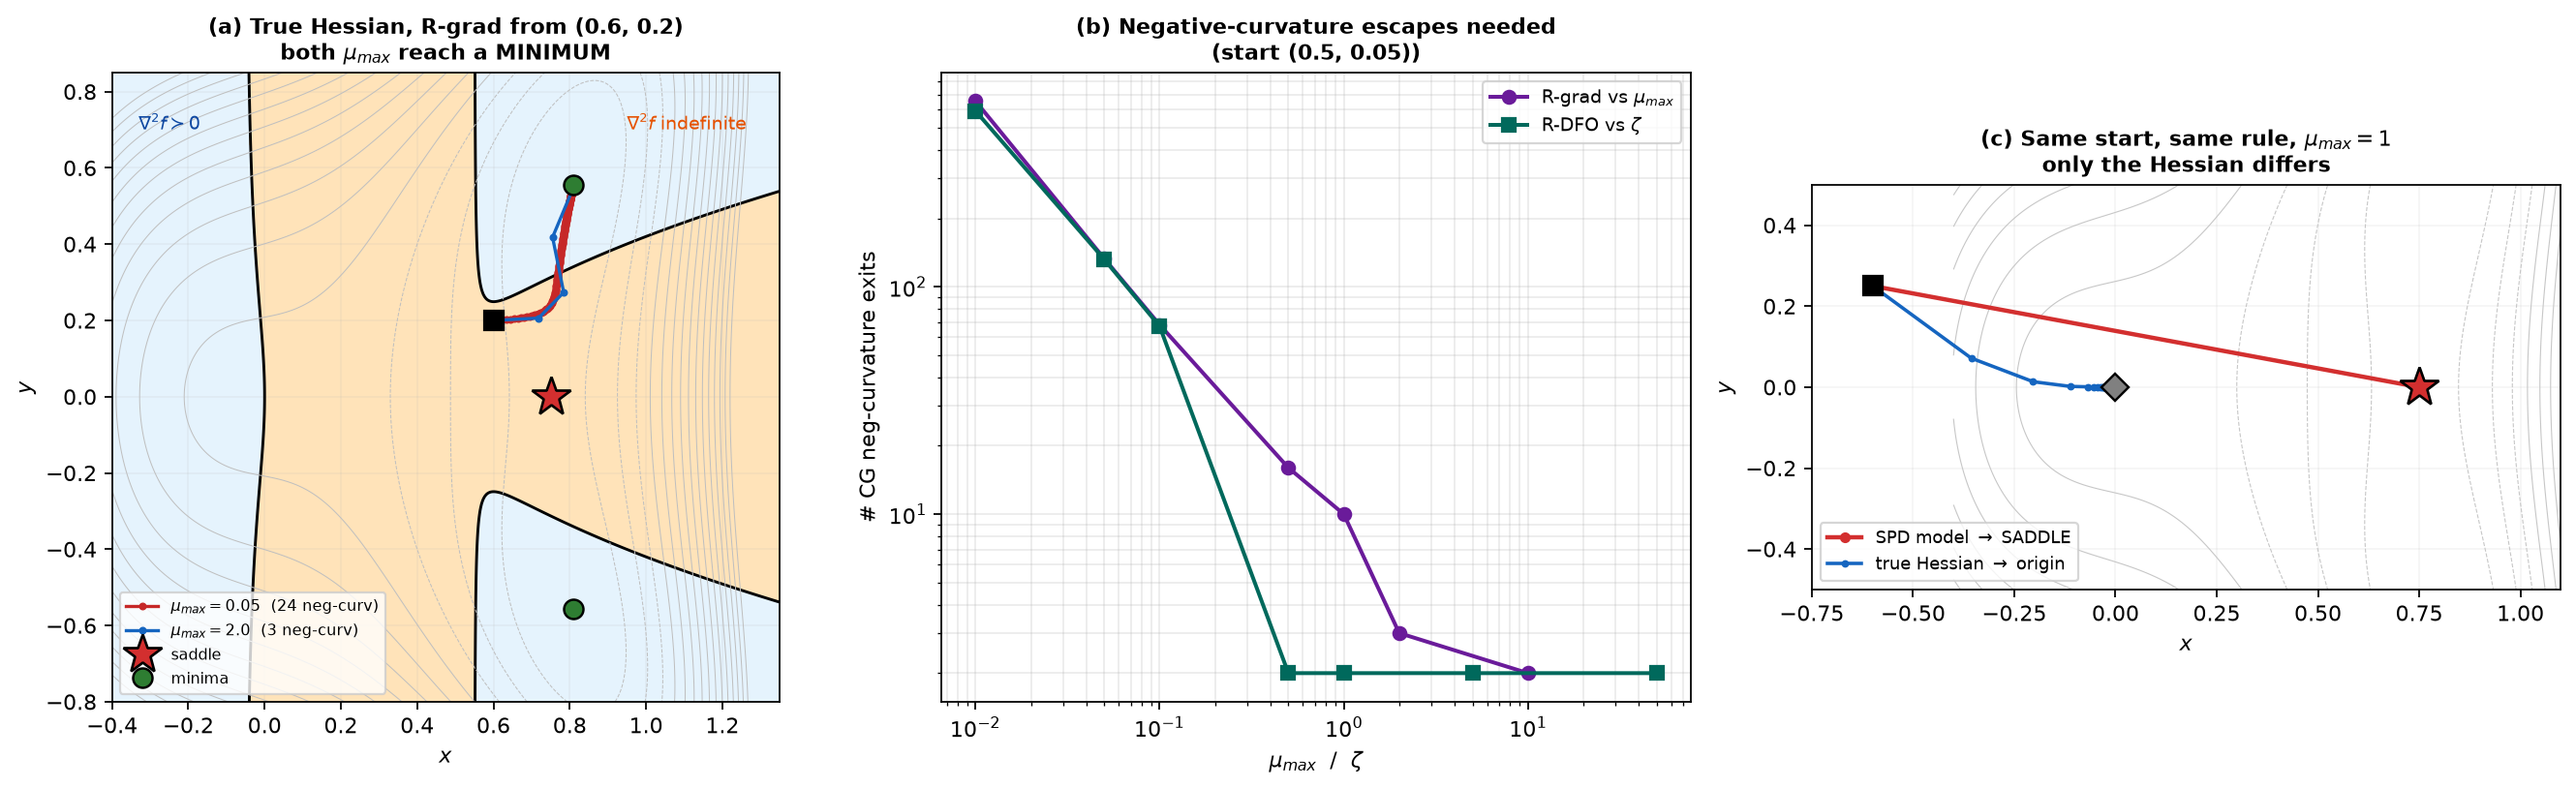
\includegraphics[width=\linewidth]{figs/true_hessian_julia.png}
  \caption{Mechanism against model Hessian on P1.
    (a) with the true Hessian and truncated CG, $\Rgrad$ reaches a minimiser for both values of
    $\overline{\mu}$, the small cap costing 24 negative-curvature exits against 3;
    (b) the number of exits against the parameter, for $\Rgrad$ against $\overline{\mu}$ and
    $\Rdfo$ against $\zeta$, decreasing by two orders of magnitude across the sweep;
    (c) the same start, the same rule and the same $\overline{\mu}$ under two model Hessians. The
    constructed positive definite model reaches the saddle, the true Hessian the degenerate point.
    Only the Hessian differs.}
  \label{fig: true hessian}
\end{figure}

\begin{figure}[htbp]
  \centering
  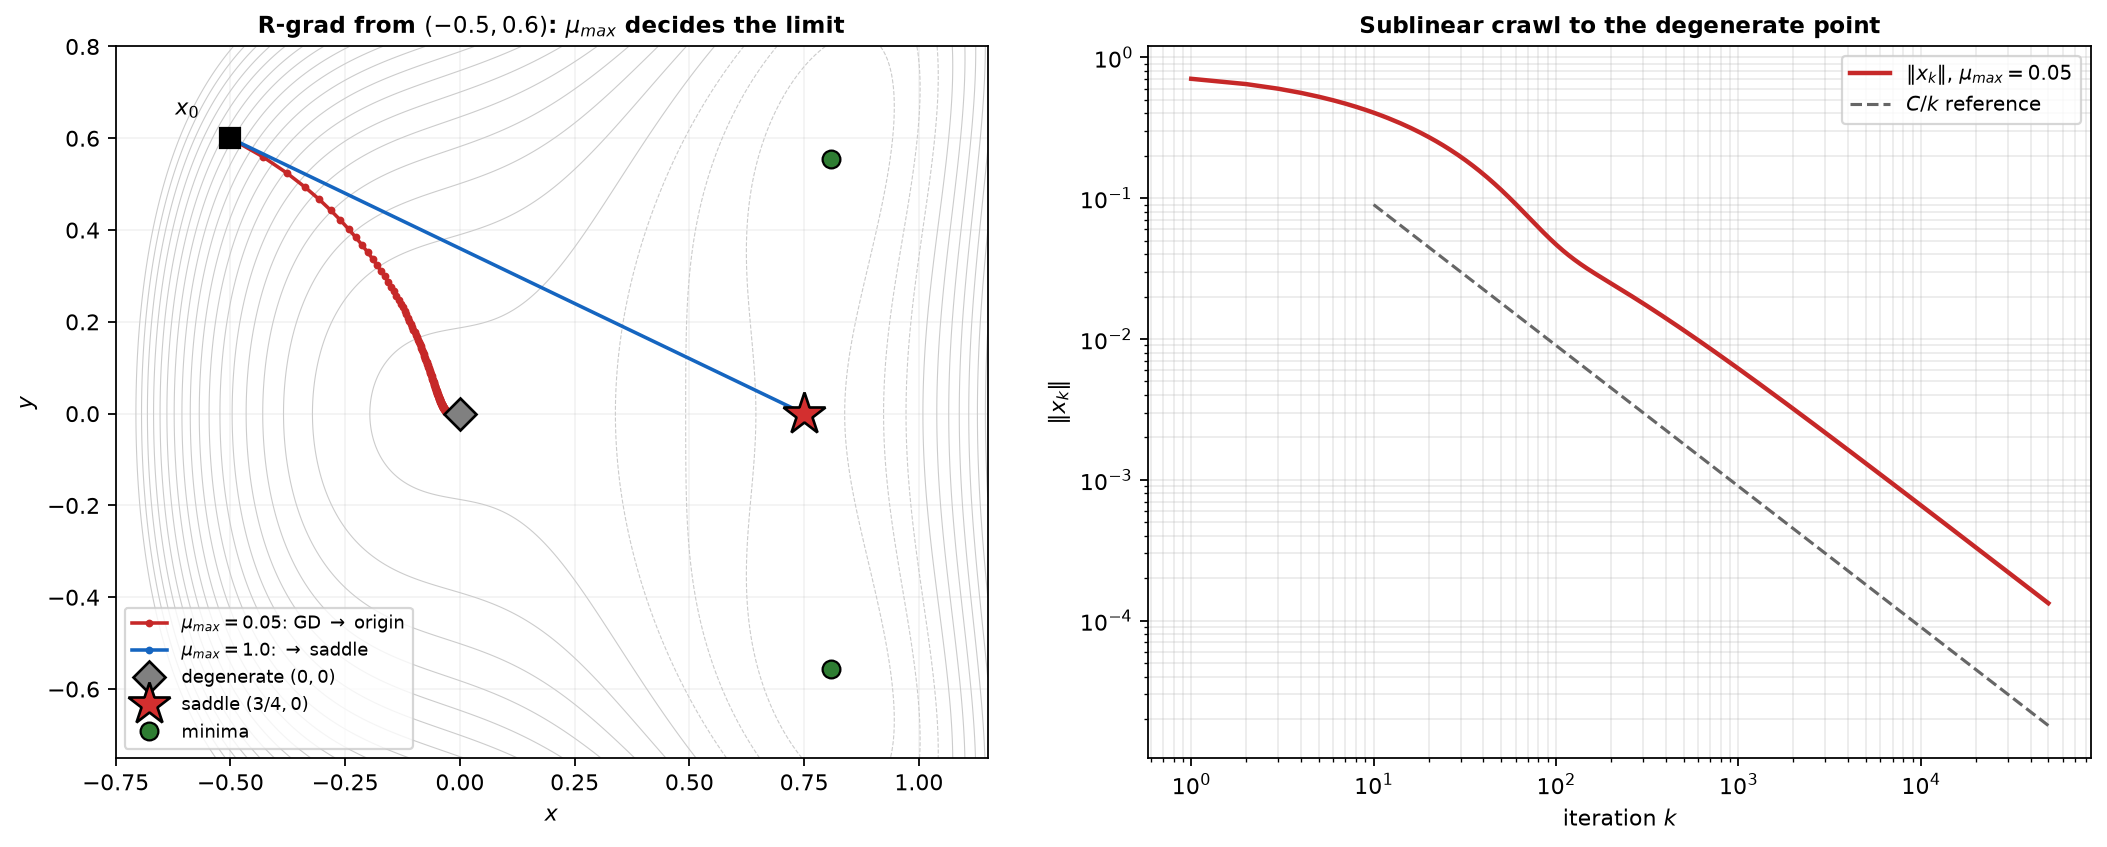
\includegraphics[width=\linewidth]{figs/rgrad_mumax_julia.png}
  \caption{$\Rgrad$ on P1 from $(-0.5, 0.6)$ under the constructed model.
    Left, the cap decides the limit: $\overline{\mu} = 1$ gives a single long step to the saddle,
    $\overline{\mu} = 0.05$ a sequence of short steps ending at the degenerate origin. Right, the
    approach to the degenerate point under the small cap is sublinear, $\norm{x_k}$ decaying at
    a rate slower than $C/k$.}
  \label{fig: rgrad mumax}
\end{figure}

Figures~\ref{fig: true hessian} and~\ref{fig: rgrad mumax} record two findings.

The first concerns the division of labour. Panel~(c) of Figure~\ref{fig: true hessian} runs the
same rule from the same point with the same parameter and changes only the model Hessian, and the
limit changes from the saddle to the degenerate point. Nothing the radius rule does can produce
that difference, which is the empirical counterpart of the claim of Part~II that the mechanism
decides the length of the step and the model decides its direction.

The second qualifies it. Panel~(b) shows that the parameter does control something measurable,
namely how often the subproblem solver must exit on negative curvature, and the count falls by
two orders of magnitude as $\overline{\mu}$ or $\zeta$ grows. A small cap forces short steps, so
the escape from the region of indefinite curvature is made in many small moves rather than in a
few large ones. The mechanism therefore governs the cost of the escape while the model governs
whether an escape occurs at all. Figure~\ref{fig: rgrad mumax} shows the limiting case, in which
the cap is small enough that the iterates never leave the neighbourhood of the degenerate point,
approaching it sublinearly. This is the failure of Part~II, Theorem on the capped rule, exhibited
on a two-dimensional problem: below the threshold the constraint binds at every iteration and the
rate collapses.

\subsection{Comparison of mechanisms}
\label{sec: exp comparison}

\begin{experiment}[Configuration matrix on the analytic problems]
\label{exp: comparison}
Run the full cross product of $\{$true, L-BFGS, SR1, constructed SPD$\}$ model Hessians,
$\{\Rdelta, \Rstep, \Rdfo, \Rgrad\}$ mechanisms and $\{$CG, exact$\}$ solvers on P1 from
$x_0 = (-0.5,0.6)$, and classify the limit.
\end{experiment}

Table~\ref{tab: config matrix} reports a representative subset. The pattern is
Claim~\ref{claim: limit}: reading down the table, the limit point tracks the model Hessian and
not the radius mechanism. The true Hessian and the quasi-Newton models deliver the iterates to
the degenerate origin under the criticality-blind and DFO-like rules; the quasi-Newton models
reach a minimiser under $\Rgrad$; and the constructed positive definite model steers every
mechanism to the saddle. The mechanisms differ by up to three orders of magnitude in iteration
count---$16$ against $18\,245$ for the same model and solver---but not in destination.

\begin{table}[htbp]
  \centering
  \caption{Configuration matrix on P1 from $x_0 = (-0.5,0.6)$, budget $60\,000$,
           $\epsilon_g = 10^{-9}$. Representative subset of the full $4\times4\times2$ matrix.
           The limit point is determined by the model Hessian, not by the radius mechanism.}
  \label{tab: config matrix}
  \small
  \begin{tabular}{lllrrl}
    \toprule
    Model & Solver & Mechanism & Iters & Dist. & Limit \\
    \midrule
    true        & CG    & $\Rdelta$              & $16$      & $1.7\times10^{-5}$  & origin \\
    true        & CG    & $\Rstep$               & $16$      & $1.7\times10^{-5}$  & origin \\
    true        & CG    & $\Rdfo\ (\zeta=1)$     & $16$      & $1.7\times10^{-5}$  & origin \\
    true        & CG    & $\Rgrad\ (\overline{\mu}=1)$ & $18\,245$ & $1.8\times10^{-5}$ & origin \\
    true        & exact & $\Rdelta$              & $17$      & $9.2\times10^{-6}$  & origin \\
    \midrule
    L-BFGS($5$) & CG    & $\Rdelta$              & $27$      & $2.5\times10^{-6}$  & origin \\
    L-BFGS($5$) & CG    & $\Rdfo\ (\zeta=1)$     & $17\,518$ & $1.8\times10^{-5}$  & origin \\
    L-BFGS($5$) & CG    & $\Rgrad\ (\overline{\mu}=1)$ & $27$ & $7.3\times10^{-9}$ & $\text{min}^{-}$ \\
    SR1         & CG    & $\Rdelta$              & $24$      & $9.4\times10^{-6}$  & origin \\
    SR1         & CG    & $\Rgrad\ (\overline{\mu}=1)$ & $15$ & $4.9\times10^{-12}$ & $\text{min}^{-}$ \\
    \midrule
    SPD (\ref{eqn: SPD model}) & CG    & $\Rdelta$          & $5$ & $2.2\times10^{-16}$ & \textbf{saddle} \\
    SPD (\ref{eqn: SPD model}) & exact & $\Rdfo\ (\zeta=1)$ & $4$ & $2.1\times10^{-17}$ & \textbf{saddle} \\
    SPD (\ref{eqn: SPD model}) & exact & $\Rgrad\ (\overline{\mu}=1)$ & $1$ & $5.0\times10^{-16}$ & \textbf{saddle} \\
    \bottomrule
  \end{tabular}
\end{table}

The last three rows deserve emphasis, since they realise Claim~\ref{claim: bad limits}. In those
runs every hypothesis of Part~I holds: the model matches $f$ to first order by construction, the
model Hessians are uniformly bounded, the exact subproblem solution satisfies Cauchy decrease
with $\mykappa{mdc} = 1$, and the mechanism is strongly admissible. Every conclusion of Part~I
is correct: $f$ decreases monotonically, every iteration is successful, $\norm{g_k} \to 0$, the
iterates converge. And the limit is a saddle. What fails is not the radius rule and not the
first-order theory, but the model Hessian, which is positive definite by construction while the
true Hessian along the trajectory has already turned indefinite.

\begin{experiment}[CUTEst comparison]
\label{exp: cutest}
Run all five mechanisms on the unconstrained problems of CUTEst~\citep{GouldOrbanToint15} with
$n \leq 1000$, using the exact Hessian and truncated CG, with a budget of $10\,000$ iterations
and $\epsilon_g = 10^{-5}$. Report performance profiles~\eqref{eqn: performance profile} on
iteration count, on function evaluations and on CPU time, and data profiles on function
evaluations. Report pairwise profiles against $\Rdelta$ as a baseline, following the
recommendation of~\citet{GouldScott16}. \placeholder
\end{experiment}

Figures~\ref{fig: profile mech} and~\ref{fig: profile zeta} establish the reporting format on
the thirty-problem set; Experiment~\ref{exp: cutest} applies it at scale. The substantive
question is whether the pattern found there---efficiency largely insensitive to the mechanism,
reliability sharply sensitive to it---persists over a large heterogeneous collection with a wide
spread of $\lambda^*_{\min}$, or whether the reliability gap closes once the budget is generous
relative to problem difficulty. Our prior, from the analytic results, is that the gap will widen
rather than close, since CUTEst contains many more nearly-singular minimisers than a hand-picked
set of textbook problems, and $\overline{\kappa} = 8/\lambda^*_{\min}$ is correspondingly larger
on those.

\begin{figure}[htbp]
  \centering
  \begin{tikzpicture}
    \begin{axis}[
        width=0.70\textwidth, height=6.6cm,
        xlabel={$\tau$ (performance ratio, iteration count)},
        ylabel={$\pi_s(\tau)$},
        xmode=log, xmin=1, xmax=110, ymin=0, ymax=1.02,
        legend pos=south east, legend style={font=\scriptsize, fill opacity=0.9,
                                             text opacity=1},
        grid=both, grid style={gray!22},
        every axis plot/.append style={line width=0.9pt},
      ]
      \input{prof_mech.tex}
    \end{axis}
  \end{tikzpicture}
  \caption{Performance profiles~\eqref{eqn: performance profile} of the five mechanisms on the
    $30$-problem analytic set of Section~\ref{sec: analytic set}, exact Hessian, truncated CG,
    $\epsilon_g = 10^{-6}$, budget $1000$ iterations. Cost measure: iteration count. The
    intercept $\pi_s(1)$ is the fraction of problems on which a mechanism is fastest and the
    right-hand asymptote its reliability. $\Rstep$ is fastest most often ($77\%$); $\Rdelta$,
    $\Rstep$ and unbounded $\Rgrad$ solve every problem, while capped $\Rgrad$ solves $93\%$.
    The capped and unbounded variants of the same rule are separated by both measures, which is
    the aggregate counterpart of the analytic results of Section~\ref{sec: exp mu}.}
  \label{fig: profile mech}
\end{figure}

\subsection{Sampling: what an iteration costs to certify}
\label{sec: res stochastic}

In the stochastic setting the radius plays the same role for sampling accuracy
that it plays for model accuracy in derivative-free work, and the question this
survey asks of it is whether the cost of an iteration depends on the radius rule.

The answer depends on the sampling rule, and two rules bracket it. A rule that
sizes the batch from the radius, $N_k \sim \Delta_k^{-2}$, makes the mechanism
pay for its own radius directly, and a criticality-anchored rule drives the
sample size up without bound near a solution while a criticality-blind one does
not. A rule that certifies the achieved decrease against its own noise behaves
differently, and the difference is the subject of the rest of this section: under
common random numbers the step length cancels between the decrease and its
standard error, leaving a cost that depends on $\norm{g_k}$ alone.

\subsubsection{Certified decrease as a sampling rule}

The natural way to couple sampling to the acceptance test is to sample until the decrease is
certified. With common random numbers, form the paired differences
\begin{equation}
  D_i = F(x_k, \xi_i) - F(x_k + s_k, \xi_i) ,
  \qquad
  N_{k+1} = \Bigl\lceil z_p^2 \hat\sigma_N^2 / \hat\delta_N^2 \Bigr\rceil ,
  \qquad z_p = \Phi^{-1}(p) ,
  \label{eqn: certified rule}
\end{equation}
where $\hat\delta_N$ and $\hat\sigma_N$ are the sample mean and standard deviation of the $D_i$.
Pairing is what makes this viable: the same $\xi_i$ is used at both points, so $D_i \to 0$
pathwise as $s \to 0$ and $\sigma_D^2 = \calO(\norm{s}^2)$, against $\calO(1)$ for independent
sampling. On~\eqref{eqn: stoch example} the measured variance ratio exceeds $7 \times 10^4$.

\begin{experiment}[Cost of certification]
\label{exp: certification cost}
  Measure $N_k$ against $\norm{g_k}$ and against $\norm{s_k}$ on~\eqref{eqn: stoch example}.
\end{experiment}

\paragraph{Finding, and it corrects a natural hope.}
One expects that since the trust region drives $\sigma_D \to 0$, a small radius makes
certification cheap. It does not. Both quantities are linear in $\norm{s}$,
\begin{equation}
  \delta_k \sim \norm{g_k}\,\norm{s_k} ,
  \qquad
  \sigma_D \sim C \norm{s_k} ,
  \qquad\Longrightarrow\qquad
  N_k \sim \frac{z_p^2 C^2 \norm{s_k}^2}{\norm{g_k}^2 \norm{s_k}^2}
        = \frac{z_p^2 C^2}{\norm{g_k}^2} ,
  \label{eqn: N cancels}
\end{equation}
and the step length cancels. Common random numbers buy a large constant, four orders of magnitude
here, and not a better rate. The total work is $\sim \varepsilon^{-2} \cdot \varepsilon^{-2} =
\varepsilon^{-4}$, matching the rate of~\citet{BlanchetCartisMenickellyScheinberg19}.

The bearing on this survey is direct. Since $N_k$ depends on $\norm{g_k}$ and not on $\Delta_k$,
the sampling cost of an iteration is \emph{insensitive to the radius rule}. The mechanisms differ
in how many iterations they take and in how large each step is, not in what each iteration costs
to certify. Any advantage a criticality-anchored rule shows in this setting therefore comes from
the iteration count alone.


Both rules are implemented and the comparison is run on the same problems with
the same mechanisms, at matched budgets, with the cost measured in term
evaluations.\provisional{} Two cautions carry into the reading. The size
in~\eqref{eqn: certified rule} rests on a normal approximation which is worst
exactly where the rule selects a small batch, and the estimator should be read as
a sequential test rather than a fixed-sample one; an empirical Bernstein
bound~\citep{MaurerPontil09} is the principled replacement, and it pays off
precisely because pairing has made the variance small.

\subsection{Extension to stochastic settings}
\label{sec: exp stochastic}

The mechanisms of this survey set the radius from quantities the algorithm measures. Under
sampling those measurements are random, and the criticality-anchored rules are the ones most
exposed, since $\Rdfo$ and $\Rgrad$ read $\norm{g_k}$ directly. This subsection reports what
happens on a one-dimensional example small enough to be understood completely, and states the
protocol for the larger study.

\subsubsection{A running example with a heavy-tailed sample minimiser}

Let
\begin{equation}
  F(x,\xi) = \xi x^2 - \ln(1+x^2) - \xi^{-\alpha} x ,
  \qquad
  f(x) = \E\bigl[F(x,\xi)\bigr] ,
  \qquad \xi \sim \mathcal{E}(\lambda) \ \text{(rate)} ,
  \label{eqn: stoch example}
\end{equation}
with $0 < \alpha < 1$. The restriction on $\alpha$ is what makes $f$ finite, and the reason is
worth recording since it is also what creates the pathology below.

\begin{lemma}[Integrability and the two moments]
\label{lem: gamma moment}
  For $X \sim \mathcal{E}(\lambda)$ and $0 < a < 1$,
  \begin{equation}
    \E\bigl[X^{-a}\bigr] = \lambda^{a}\,\Gamma(1-a) \;<\; \infty .
    \label{eqn: gamma moment}
  \end{equation}
  The moment is infinite for $a \geq 1$.
\end{lemma}

\begin{proof}
  With the substitution $u = \lambda x$,
  \begin{equation*}
    \E\bigl[X^{-a}\bigr]
      = \lambda\int_0^\infty x^{-a} e^{-\lambda x}\,dx
      = \lambda \cdot \lambda^{a} \cdot \frac{1}{\lambda}
        \int_0^\infty u^{-a} e^{-u}\,du
      = \lambda^{a}\,\Gamma(1-a) ,
  \end{equation*}
  the integral being the Gamma function at $1-a$, which converges exactly for $a < 1$. The
  convergence is worth seeing directly, since it is where the two regimes separate. On $(0,1)$
  the integrand is bounded by $u^{-a}$, whose integral is $1/(1-a)$, finite precisely because
  $a < 1$; on $(1,\infty)$ it is bounded by $e^{-u}$, which converges for every $a$. The
  singularity at the origin is therefore the only obstruction, and it is integrable up to
  $a = 1$ and not beyond.
\end{proof}

We take $\alpha = \lambda = \tfrac12$ throughout, for which
\begin{equation}
  \E[\xi] = 2 ,
  \qquad
  \Var[\xi] = 4 ,
  \qquad
  \E\bigl[\xi^{-1/2}\bigr] = \tfrac{1}{\sqrt2}\,\Gamma(\tfrac12) = \sqrt{\pi/2} = 1.2533141 ,
  \label{eqn: stoch constants}
\end{equation}
so that
\begin{equation}
  f(x) = 2x^2 - \ln(1+x^2) - 1.2533141\,x ,
  \qquad
  x^* = 0.5173980 ,
  \qquad
  f(x^*) = -0.3502656 .
  \label{eqn: stoch f}
\end{equation}

The example has three properties that make it the right test bed for this survey.

\paragraph{It is benign in the mean and explicit in the constants of Part~II.}
Differentiating twice,
$f''(x) = 4 - 2(1-x^2)/(1+x^2)^2$, which attains its minimum $2$ at $x = 0$ and its maximum
$17/4$ at $x = \pm\sqrt{3}$. So $f$ is globally strongly convex with
\begin{equation}
  m = 2 , \qquad M = \tfrac{17}{4} , \qquad
  \kbar = \frac{4}{m} = 2 ,
  \label{eqn: stoch constants mM}
\end{equation}
and the constant that Part~II shows to be unknowable in general is here available in closed form.
The example is therefore one of the few places where the side conditions $\zeta > \kbar$ and
$\overline{\mu} > \kbar$ can be checked rather than assumed, which is what makes the thresholds
below measurable.

\paragraph{The pathology sits in the sample problem, not in $f$.}
Each realisation $F(\cdot,\xi)$ is itself a smooth one-dimensional function, but the family is far
more dispersed than the mean suggests, since a small draw flattens the quadratic term and steepens
the linear one at the same time. Figure~\ref{fig: stoch example}(a) shows sixty realisations
against $f$.

\begin{proposition}[Infinite-mean sample minimiser]
\label{prop: infinite mean}
  For $\alpha = \lambda = \tfrac12$ the minimiser $\hat x$ of the single-sample problem
  $\min_x F(x,\xi)$ satisfies $\hat x(\xi) \sim \tfrac12\xi^{-3/2}$ as $\xi \to 0^+$ and
  \begin{equation}
    \Prob(\hat x > \tau) \;\sim\; \lambda\,(2\tau)^{-2/3}
    \qquad (\tau \to \infty) ,
    \label{eqn: xhat tail}
  \end{equation}
  a power law of index $2/3 < 1$, so that $\E[\hat x] = +\infty$.
\end{proposition}

\begin{proof}
  Stationarity $\partial_x F(x,\xi) = 0$ reads
  $2\xi x - 2x/(1+x^2) - \xi^{-\alpha} = 0$, and clearing the denominator gives the cubic
  \begin{equation}
    2a\,x^3 - b\,x^2 + 2(a-1)\,x - b = 0 ,
    \qquad a = \xi , \quad b = \xi^{-\alpha} .
    \label{eqn: xhat cubic}
  \end{equation}
  As $\xi \to 0^+$ the two coefficients move in the same direction, $a \to 0$ flattening the
  curvature and $b = \xi^{-1/2} \to \infty$ steepening the slope. Substituting the ansatz
  $x = C\xi^{-3/2}$ and collecting the dominant order $\xi^{-7/2}$ leaves $2C^3 - C^2 = 0$, whence
  $C = \tfrac12$, the remaining terms being $\calO(\xi^{-3/2})$. For the tail, $\hat x$ is
  decreasing in $\xi$ near the origin, so
  $\Prob(\hat x > \tau) = \Prob\bigl(\xi < (2\tau)^{-2/3}(1+o(1))\bigr)$, and
  $\Prob(\xi < u) = 1 - e^{-\lambda u} \sim \lambda u$ as $u \to 0$ gives
  \eqref{eqn: xhat tail}. A tail index below $1$ makes the mean infinite.
\end{proof}

Figure~\ref{fig: stoch example}(c) and~(d) display the map $\xi \mapsto \hat x$ and the empirical
tail against~\eqref{eqn: xhat tail} over four decades.

\paragraph{The radius is what tames it.}
This is the point of the example for the present survey. A method that draws one fresh sample per
iteration and moves toward that sample's minimiser inherits the infinite mean, and no amount of
averaging within an iteration removes it, since the pathology is in the minimiser rather than in
the objective. A trust-region radius truncates each such step, so the iterate averages the samples
across iterations instead of chasing them one at a time. \emph{The radius performs the variance
reduction that the sample size cannot afford}, and it does so by step-length truncation rather
than by any property of a particular rule, so it holds for every mechanism that drives
$\Delta_k \to 0$. Whether the truncation is set from the previous radius, from the realised step
or from a noisy criticality measure is exactly the question the rest of this subsection asks.

\begin{figure}[htbp]
  \centering
  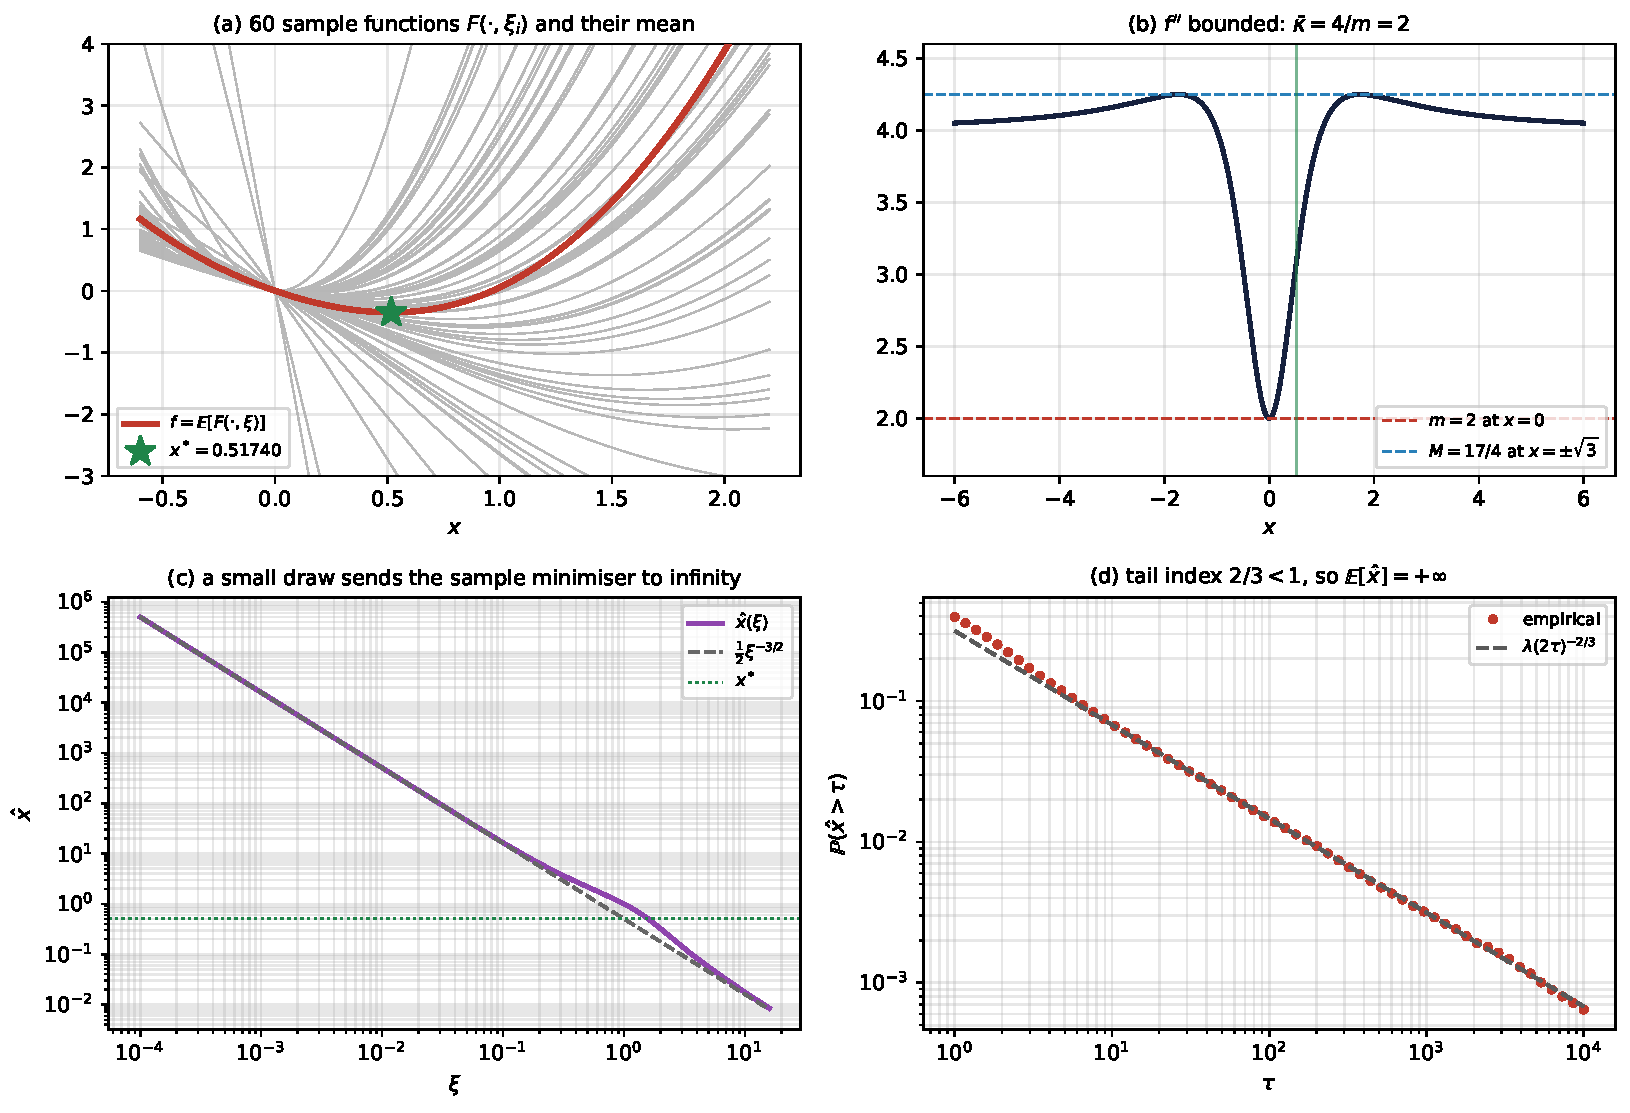
\includegraphics[width=\linewidth]{figs/stoch_example.pdf}
  \caption{The example~\eqref{eqn: stoch example} with $\alpha = \lambda = \tfrac12$.
    (a) sixty realisations $F(\cdot,\xi_i)$ against the mean $f$, whose minimiser is
    $x^* = 0.5173980$;
    (b) $f''$, bounded between $m = 2$ and $M = 17/4$, so that $\kbar = 4/m = 2$ is available in
    closed form;
    (c) the map $\xi \mapsto \hat x$ of~\eqref{eqn: xhat cubic} against the asymptote
    $\tfrac12\xi^{-3/2}$ of Proposition~\ref{prop: infinite mean};
    (d) the empirical tail of $\hat x$ over $2 \times 10^5$ draws against
    $\lambda(2\tau)^{-2/3}$, of index $2/3$.}
  \label{fig: stoch example}
\end{figure}

\subsubsection{Two caveats the experiments expose}

\paragraph{The normal approximation is the weak point.}
Rule~\eqref{eqn: certified rule} rests on $\hat\delta_N \approx \mathcal{N}(\delta,
\sigma_D^2/N)$, and two things go wrong at once. The rule selects small $N$ exactly when the
decrease is large, which is where the approximation is worst, and $D_i$ inherits the heavy left
tail of $\xi^{-\alpha}$, with measured excess kurtosis of order $10^4$. For a theorem, $z_p$
should be replaced by an empirical Bernstein bound~\citep{MaurerPontil09}, which is worth
invoking precisely because pairing has made $\hat\sigma_N$ small, a variance-dependent bound
paying off when the variance is small.

\paragraph{The rule is a sequential test, and must be read as one.}
Read as \emph{fix $N$, accept if $\hat\delta_N > 0$} the rule is badly miscalibrated: at $N = 10$
it accepts steps that truly increase $f$ about $36\%$ of the time, against a nominal $1-p = 0.1$.
Read as a sequential test, sampling until either $\hat\delta_N \geq z_p\hat\sigma_N/\sqrt{N}$ or
$\hat\delta_N \leq 0$, calibration is restored. The price is conservatism, good steps being
accepted between $25\%$ and $55\%$ of the time. For a trust-region method that asymmetry is the
right one, since rejecting a good step costs one iteration and a contraction while accepting a
bad one corrupts the potential function.

\subsubsection{What survives of the martingale framework}

\begin{experiment}[Fixed and variable budgets]
\label{exp: stoch budgets}
  On~\eqref{eqn: stoch example}, compare the three radius rules with truncated CG and the true
  Hessian against stochastic gradient and \textsc{Adam}, at fixed budgets
  $N \in \{4,16,64\}$ drawn afresh each iteration, and then under a geometric ramp
  $N_k = \lceil N_0 r^k \rceil$, a radius-tied budget, and the certified rule
  of~\eqref{eqn: certified rule}. Report distance to $x^*$ against total replications.
\end{experiment}

The potential $\Phi_k = \nu f(X_k) + (1-\nu)\Delta_k^2$ and the accuracy condition of the
framework of~\citet{ChenMenickellyScheinberg18} are agnostic to \emph{how} the required
probability is achieved, needing only that it hold conditionally on the past, so an adaptive rule
is a constructive way of delivering it. The budget bound goes through unchanged, its proof using
only the supermartingale property and monotone convergence.

What does not survive is the renewal argument. The expected stopping time
$\E[\tau_n] = p/(2p-1)$ requires the increments to be independent and identically distributed with
a \emph{constant} $p$, which is what makes the associated walk homogeneous. Under
\eqref{eqn: certified rule} the sample size is computed from $\hat\delta_N$ and $\hat\sigma_N$,
both measurable with respect to the past, so
$p_k = \Prob(W_{k+1} = 1 \mid \calF_k)$ is random and adapted, the walk is inhomogeneous, and the
renewal lemma fails. The obstruction is the adaptivity of $p_k$ and not the sampling as such: it
would arise for any rule that reads the data to decide how much data to read.

The repair is a floor. Take $N_k = \max\{N_k^{\text{rule}}, N_k^{\text{floor}}\}$ with the floor
chosen so that $p_k \geq \underline p > 1/2$ always, generate one uniform $U_{k+1}$ per step and
set $W_{k+1} = +1$ when $U_{k+1} \leq p_k$ and $\underline W_{k+1} = +1$ when
$U_{k+1} \leq \underline p$. Since $p_k \geq \underline p$ almost surely, $W_{k+1} \geq
\underline W_{k+1}$ pathwise, and the homogeneous walk dominates.

\subsubsection{The radius as a random walk, and which rules admit the picture}

The martingale analyses read the radius as a random walk, and the reading is worth stating
carefully, because it holds for one of the five mechanisms exactly, for a second after a change
of variable, and for the remaining three not at all. Which of the three cases a rule falls into
turns out to be the same classification as in Part~II.

\paragraph{The picture.}
Under $\Rdelta$ the radius is multiplied at every iteration by one of finitely many factors, so
with $\gamma_1 = \gamma_3^{-1}$ for simplicity,
\begin{equation}
  \Delta_k = \Delta_0 \, \gamma_3^{\,Z_k} ,
  \qquad
  Z_{k+1} = Z_k + W_{k+1} ,
  \qquad W_{k+1} \in \{-1,+1\} ,
  \label{eqn: radius walk}
\end{equation}
and $Z_k$ is a walk on $\mathbb{Z}$. The increment is $+1$ when the model is accurate and the
iteration successful, which happens with conditional probability $p$, and $-1$ otherwise. The
whole apparatus of~\citet{BlanchetCartisMenickellyScheinberg19} rests
on~\eqref{eqn: radius walk}: the expected time to return to a level is read off the walk, and the
renewal identity $\E[\tau_n] = p/(2p-1)$ requires the increments to be independent and identically
distributed with a \emph{constant} $p$, which is what makes $Z_k$ homogeneous and licenses Wald's
identity.

\paragraph{Two of the five rules do not admit it.}
The representation~\eqref{eqn: radius walk} needs $\Delta_{k+1}/\Delta_k$ to take finitely many
values independent of the state. That fails for $\Rstep$, where
$\Delta_{k+1} = \gamma\norm{s_k}$ and the ratio $\norm{s_k}/\Delta_k$ lies anywhere in $(0,1]$
according to whether the constraint binds, and it fails for $\Rdfo$, whose second branch is
selected by the test $\Delta_k > \zeta\norm{g_k}$ and therefore by the state. In both cases
$\log\Delta_k$ is a walk with state-dependent increments, which is exactly what the renewal
argument cannot accommodate. $\Rrtr$ inherits the difficulty from $\Rstep$.

\paragraph{$\Rgrad$ admits it, on the multiplier.}
Here the change of variable is the one Part~II already makes. The radius
$\Delta_k = \mu_k\norm{g_k}$ is a product of a quantity the rule controls and one the problem
controls, and it is the first factor that walks:
\begin{equation}
  \mu_k = \mu_0\,\gamma_3^{\,Z_k} ,
  \qquad
  \log\Delta_k = \log\mu_k + \log\norm{g_k} .
  \label{eqn: mu walk}
\end{equation}
The multiplier is therefore a homogeneous walk in exactly the sense~\eqref{eqn: radius walk}
requires, while the radius is that walk plus a state-dependent drift. What makes this more than a
bookkeeping observation is that $\mu_k = \theta_k = \Delta_k/\norm{g_k}$ is the radius-to-%
criticality ratio, so the walk is on the very quantity whose crossing of $\kbar$ decides
inactivity. Figure~\ref{fig: rgrad walk} displays the three regimes.

\begin{figure}[htbp]
  \centering
  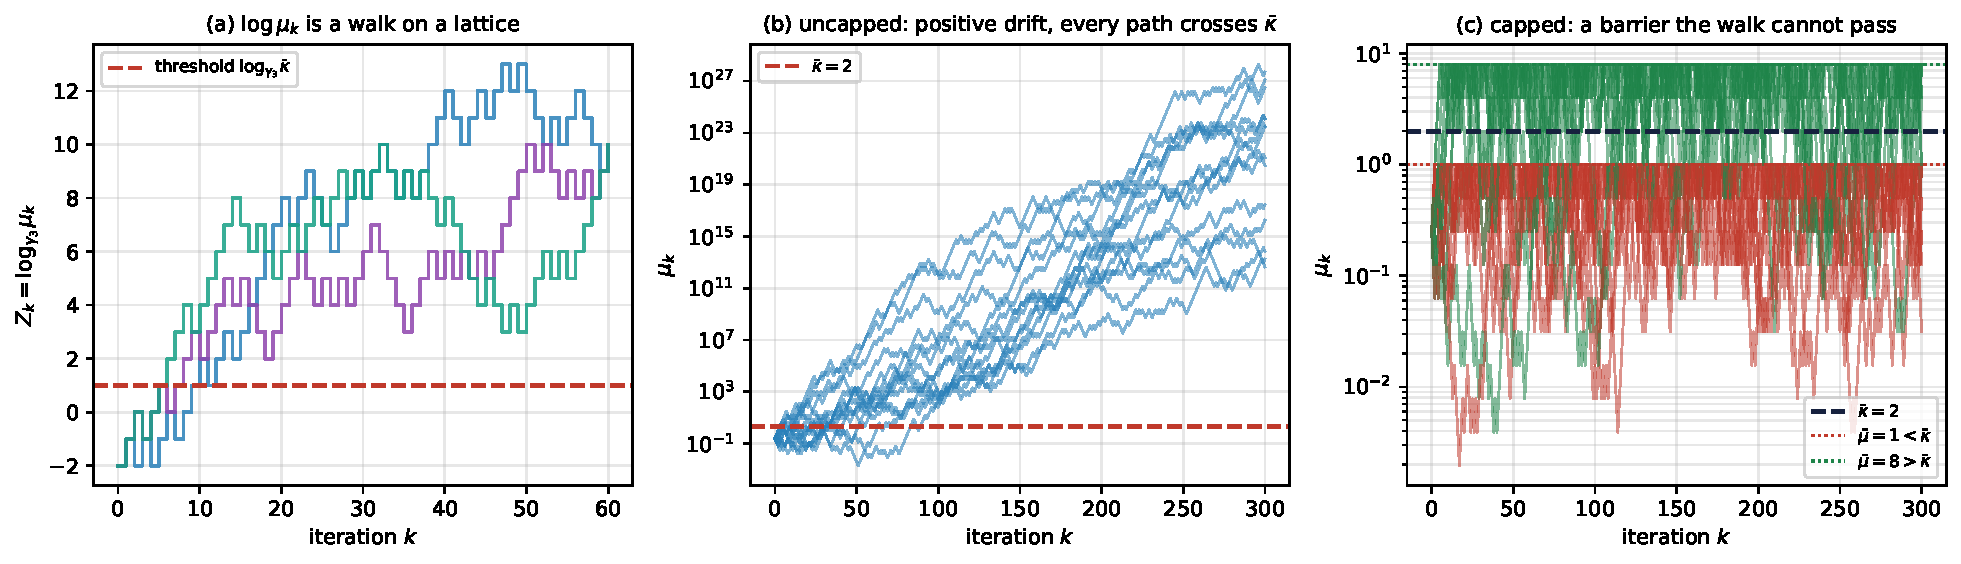
\includegraphics[width=\linewidth]{figs/rgrad_walk.pdf}
  \caption{The multiplier of $\Rgrad$ as a random walk, with $\gamma_1 = 1/2$, $\gamma_3 = 2$,
    $\mu_0 = 1/4$ and $\kbar = 2$ as in~\eqref{eqn: stoch constants mM}.
    (a) $Z_k = \log_{\gamma_3}\mu_k$ moves by $\pm1$ on a lattice;
    (b) uncapped, with the upward drift of the eventual very successful regime, every path
    crosses $\kbar$ and none returns below it for long;
    (c) capped, the cap acting as a barrier. Above $\kbar$ the barrier is harmless, below it the
    walk saturates at $\overline{\mu}$ and can never cross.}
  \label{fig: rgrad walk}
\end{figure}

\paragraph{What the picture explains.}
Read this way the three results of Part~II on the gradient-scaled rule become three statements
about one walk, and each becomes visible rather than merely provable.

Uncapped, and in the regime where every iteration is eventually very successful, the increment is
$+1$ whenever the step is long, so the walk has positive drift and crosses any fixed level almost
surely. The threshold $\kbar$ is a level like any other, which is why the inactivity result needs
no hypothesis about its value: a drifting walk on $\mathbb{Z}$ does not care where the line is
drawn. This is the random-walk form of Part~II's theorem on the uncapped rule.

Capped, the rule adds an absorbing barrier at $\log_{\gamma_3}\overline{\mu}$. The walk saturates
there, which is the content of the identification $L = \overline{\mu}$ in Part~II's theorem on the
capped rule, and it crosses $\kbar$ if and only if the barrier is above the threshold. The failure
below the threshold is then not a slow crossing but no crossing at all, which is why the
constraint binds at \emph{every} sufficiently large iteration rather than infinitely often.

For $\Rdelta$ the walk is on $\Delta_k$ rather than on $\theta_k$, so crossing a level tells one
nothing about inactivity, the comparison with $\norm{g_k}$ never being made. The rule gets the
homogeneous walk and loses the quantity worth walking on. That is the anchoring trade of Part~II,
arriving here as a choice of state variable.

\begin{remark}[The obstruction is adaptivity, not sampling]
\label{rem: adaptivity obstruction}
  The renewal argument fails under~\eqref{eqn: certified rule} for a reason unrelated to the
  mechanism, and it is worth separating the two failures. Since $N_{k+1}$ is computed from
  $\hat\delta_N$ and $\hat\sigma_N$, both $\calF_k$-measurable, the conditional probability
  $p_k = \Prob(W_{k+1} = 1 \mid \calF_k)$ is itself random and adapted, the walk is inhomogeneous,
  and $\E[\tau_n] = p/(2p-1)$ is unavailable. This would arise for \emph{any} rule that reads the
  data to decide how much data to read, whatever the radius mechanism, and the floor
  of~\S\ref{sec: exp stochastic} repairs it by coupling to a homogeneous walk from below.

  The mechanism-dependent failure is the other one. For $\Rstep$ and $\Rdfo$ the increments are
  state-dependent even with $p$ constant and even with no sampling at all, so no floor recovers a
  homogeneous walk. A rate analysis for those rules must therefore be built on something other
  than the renewal identity, and to our knowledge has not been.
\end{remark}

\begin{remark}[Why this matters for the survey]
\label{rem: stochastic and anchoring}
  The floor is a lower bound on the sampling effort, and the criticality-anchored rules are the
  ones that make it expensive. By~\eqref{eqn: N cancels} the certification cost grows as
  $\norm{g_k}^{-2}$, while $\Rdfo$ and $\Rgrad$ tie the radius to $\norm{g_k}$ and so keep taking
  steps whose certification is hardest exactly where the gradient is smallest. A fixed-factor
  rule does not read $\norm{g_k}$ and is indifferent. This is the same trade recorded throughout
  Part~II, arriving here as a budget rather than as a constant of the solution, and it is the
  reason the stochastic comparison is worth running rather than inferring.
\end{remark}

\subsubsection{Protocol for the large-scale study}

\begin{experiment}[Subsampled logistic regression]
\label{exp: stochastic}
Minimise the regularised logistic loss
\begin{equation}
  f(w) = \frac{1}{N}\sum_{i=1}^{N}
    \log\bigl(1 + \exp(-b_i\, a_i^\top w)\bigr) + \frac{\lambda}{2}\norm{w}^2
  \label{eqn: logistic}
\end{equation}
on datasets from LIBSVM~\citep{ChangLin11}, with the gradient and Hessian estimated from
independent subsamples of sizes $N_g$ and $N_H$. Sweep the sample sizes and the mechanism, and
report the number of effective passes over the data required to reach a fixed accuracy.
\placeholder
\end{experiment}

Two opposing effects are plausible and the experiment is designed to separate them. Coupling the
radius to an estimate that fluctuates may destabilise the method, expanding the radius on
iterations where the gradient estimate happens to be large. Alternatively the coupling may act as
an automatic step-size control, since the estimate does not shrink below the noise floor and
therefore keeps the radius bounded away from zero, which is what avoids the stagnation documented
in Section~\ref{sec: setup}. The theory to compare against is
that of~\citet{BandeiraScheinbergVicente14} and~\citet{ChenMenickellyScheinberg18} for
convergence and~\citet{BlanchetCartisMenickellyScheinberg19} for the rate, all carried out for
fixed-factor rules. Whether their conclusions extend to a radius set from a noisy measurement
appears to be open, and a negative finding here would be informative.

A secondary design, closer to Part~II, fixes the sample sizes and varies $\overline{\mu}$, testing
whether the threshold of Experiment~\ref{exp: mu} persists under noise and whether it moves with
the noise level. \placeholder

%=======================================================================
\section{Threats to validity}
\label{sec: threats}
%=======================================================================

We list the principal limitations, in the spirit of~\citet{BeiranvandHareLucet17}.

\paragraph{The analytic problems are chosen to separate the mechanisms.}
P1, P2 and P3 were constructed to exhibit specific pathologies. They establish that the failures
are possible and identify the responsible ingredient, but they say nothing about frequency.
Conclusions about typical behaviour must come from Experiment~\ref{exp: cutest}, and no claim
about typical behaviour should be read into the analytic results.

\paragraph{Parameters are held fixed rather than tuned.}
Fixing $\gamma_i$ and $\eta_i$ across mechanisms makes the comparison interpretable but is not
obviously fair: a mechanism whose natural operating point differs from the classical one is
handicapped. The alternative---tuning each mechanism separately---measures tuning effort as
much as algorithmic merit. We have chosen the first and flag it explicitly.

\paragraph{Iteration counts are an imperfect cost measure.}
On the analytic problems, function and gradient evaluations are essentially free, so iteration
count is the only meaningful measure. On real problems the appropriate measure depends on the
relative cost of evaluations and linear algebra, which is why Experiment~\ref{exp: cutest}
reports three separate profiles rather than one.

\paragraph{The stagnation criterion is implementation-dependent.}
Our classification of a run as stagnated depends on a threshold relative to the rounding level
of $f$. A different threshold would move some runs between the stagnated and budget-exhausted
categories. The qualitative finding---that criticality-anchored rules can drive the radius below
the level at which $\rho_k$ carries information---is robust, but the counts are not.

\paragraph{Single starting point per analytic problem.}
The analytic experiments use one starting point per problem, chosen to sit in the relevant
basin. Results near a separatrix are sensitive to the starting point, and a fuller study would
sample starting points and report distributions.

%=======================================================================
\section{Conclusions}
\label{sec: conclusions}
%=======================================================================

Three findings emerge from the analytic portion of the campaign.

\emph{The mechanism sets the step length; the model sets the direction.} Across the
configuration matrix of Experiment~\ref{exp: comparison} the limit point tracks the model
Hessian and never the radius rule. Mechanisms differ by orders of magnitude in speed and not at
all in destination. This is structural rather than accidental: the radius rule chooses how far
along $s_k$ to travel, while the direction is determined by $B_k$ and the subproblem solver.
It follows that no radius rule can repair a model that misreports curvature, and that a
comparison of mechanisms on problems where the trust region is rarely the binding constraint
measures very little.

\emph{The user parameters of the criticality-anchored rules have real thresholds, and the safe
side is not the conservative side.} Both $\zeta$ and $\overline{\mu}$ exhibit a threshold below
which the trust-region constraint never stops binding; the threshold scales with
$1/\lambda^*_{\min}$ as Part~II predicts. Because $\lambda^*_{\min}$ is a property of the
solution, no admissible value can be chosen a priori. Worse, the intuition that a small
parameter is the cautious choice is exactly backwards: with a quasi-Newton model and a
truncated-CG solver, a small cap makes the method gradient descent and changes the limit from a
minimiser to a degenerate point. The unbounded $\Rgrad$ variant, which grows $\mu_k$ past any
threshold unconditionally, is the one rule in the survey that escapes this by construction, and
our results support preferring it.

\emph{First-order diagnostics cannot detect the failures that matter.} In the runs that converge
to a saddle, every quantity a practitioner monitors is healthy. In the runs that degenerate to
gradient descent, the same is true. The distinguishing measurements are the fraction of
iterations on which the constraint binds, the cosine between the step and the negative gradient,
and the leftmost eigenvalue of the true Hessian along the trajectory---none of which is normally
recorded. A modest recommendation from this study is that trust-region codes should expose the
first two, which are free to compute.

The large-scale portion of the campaign---Experiments~\ref{exp: cutest},
\ref{exp: interaction full} and~\ref{exp: stochastic}---remains to be run, and we expect it to
sharpen rather than overturn these conclusions. The specific open question we consider most
interesting is the one raised in Section~\ref{sec: stochastic lit}: whether tying the radius to
a noisy criticality measure stabilises or destabilises a subsampled method. The existing
probabilistic-model analyses do not cover the criticality-anchored rules, and the answer is not
clear from the deterministic theory.

%=======================================================================
\section*{Acknowledgements}
%=======================================================================

\TODO{funding, computing resources, referees}

\bibliography{References,References-numerical-v2}

%=======================================================================
%   APPENDIX
%=======================================================================
\appendix

\section{Basic trust-region algorithm} \label{app: BTR algorithm}

\begin{algorithm}[H]
    \small
    \SetAlgoLined
    \DontPrintSemicolon

    \textbf{Step 0: Initialisation.} Choose $\eta \geq 0$. Set $x_0 \in \R^p$, $\Delta_0 \in (0, \infty)$. Compute $f(x_0)$ and set $k = 0$. \; ~\\

    \textbf{Step 1: Model definition and step computation.} Define a local model $m_k$ of $f$ in the neighbourhood $\calB_k$. \; ~\\

    \textbf{Step 2: Model minimisation.} Compute a step $s_k$ that sufficiently reduces $m_k$ with $x_k + s_k \in \calB_k$, and define $x_k^{\mathrm{cand}} = x_k + s_k$. \; ~\\

    \textbf{Step 3: Acceptance of the trial point.} Compute $f(x_k^{\mathrm{cand}})$ and define
    \begin{equation}
        \rho_k = \frac{f(x_k) - f(x_k^{\mathrm{cand}})}{m_k(0) - m_k(s_k)}.
        \label{eqn:definition rho}
    \end{equation}
    If $\rho_k \geq \eta$, set $x_{k+1} = x_k + s_k$; otherwise $x_{k+1} = x_k$. \; ~\\

    \textbf{Step 4: Trust-region radius update.} Compute $\Delta_{k+1}$ according to some update rule. \; ~\\

    \textbf{Step 5: Next iteration.} Increment $k$ by 1 and repeat \textbf{Steps 1 to 5} while some stopping criterion is not met. \;

    \caption{Basic trust-region algorithm (BTR).}
    \label{alg:generic BTR}
\end{algorithm}




%=======================================================================
\section{Statements imported from Part~II}
\label{app: imported}
%=======================================================================

The body refers to the following, all of them established in Part~II. They are
restated here, without proof, so that this paper can be read on its own and so
that every cross-reference resolves. The numbering is local.

\begin{cond}{C.Sg}[step bounded by the gradient]
\label{cond: s_k bounded by g_k}
    There are $\delta^{(s)} > 0$ and $\kbar > 0$ with
    $\norm{x_k - x^*} \leq \delta^{(s)} \Rightarrow \norm{s_k} \leq \kbar\norm{g_k}$.
\end{cond}

\begin{cond}{C.Inx}[subproblem inexactness]
\label{cond:inexactness}
    Whenever the trust-region constraint is inactive,
    \begin{equation*}
      \norm{H_ks_k + g_k} \;\leq\; \xi_k\norm{g_k},
      \qquad \xi_k \in [0,1), \quad \xi_k \to 0 .
    \end{equation*}
\end{cond}

\begin{cond}{C.Lb2}[second-order lower bound on the radius]
\label{condition: lower bound Delta (2nd order)}
    $\Delta_k \geq \mykappa{lbd}^{(2)} \varsigma_k / M_k^{(2)}$ with
    $\varsigma_k = \min_{j\leq k}\tau_j$ and $\{M_k^{(2)}\}$ non-decreasing and
    dominating the thresholds of the second-order successful-iteration lemma.
\end{cond}

\begin{assum}{H.Hs}[Hessian--step residual condition]
\label{as: Hessian-step residual condition}
    \begin{equation*}
      \frac{\norm{(H_k - \nabla^2 f(x_k))s_k}}{\norm{s_k}} \longrightarrow 0
      \qquad\text{whenever}\qquad \norm{g_k} \to 0 .
    \end{equation*}
\end{assum}

\begin{assum}{a.Mx}[maximum of Cauchy and eigenpoint decrease]
\label{as: max Cauchy/eigen decrease}
    The model decrease is at least $\tfrac{\mykappa{moc}}{2}$ times the larger of
    the Cauchy decrease and $\max(0,-\lambda_k^-)\Delta_k^2$.
\end{assum}

\begin{assum}{a.Sc}[side conditions on $\zeta$ and $\overline{\mu}$]
\label{as: conditions on constants criticality related updates}
    For the criticality-anchored rules the constants satisfy $\zeta > \kbar$ and
    $\overline{\mu} > \kbar$.
\end{assum}

\begin{assum}{a.Sob}[step on the boundary under negative curvature]
\label{as: boundary step}
    When $\lambda_k^- < 0$ then $\norm{s_k} = \Delta_k$.
\end{assum}

\begin{remark}[which solvers supply \ref{as: boundary step}]
\label{rem: sob solvers}
    It holds for the eigenpoint and for any exact solution with indefinite
    $H_k$. For a truncated conjugate-gradient step it holds when the Krylov
    subspace generated by $g_k$ meets the negative-curvature subspace, and not
    otherwise.
\end{remark}

\begin{remark}[why the boundary and not a fraction of it]
\label{rem: sob must be one}
    Relaxing \ref{as: boundary step} to
    $\norm{s_k} \geq \mykappa{sob}\Delta_k$ with $\mykappa{sob} < 1$ permits a
    geometric decay of the radius while $\tau_k$ stays bounded away from zero, and
    Condition~\ref{condition: lower bound Delta (2nd order)} then fails.
\end{remark}

\begin{proposition}[local inequalities at a strong minimiser]
\label{prop: inequalities for positive definite Hessian}
    With $\nabla^2 f(x^*) \succ 0$ there are $0 < m \leq M$ and a ball
    $B(x^*,\Delta_*)$ on which $mI \preceq \nabla^2 f \preceq MI$, and on which
    $m\norm{x - x^*} \leq \norm{g(x)} \leq M\norm{x-x^*}$ and
    $\tfrac12 m\norm{x-x^*}^2 \leq \abs{f(x)-f(x^*)} \leq \tfrac12 M\norm{x-x^*}^2$.
\end{proposition}

\begin{remark}[$m$ and $M$ against the eigenvalues]
\label{rem: m M versus eigenvalues}
    $m$ and $M$ bound the Hessian on a neighbourhood, so
    $0 < m \leq \lambda^*_{\min} \leq \lambda^*_{\max} \leq M$, with the gap made
    as small as desired by shrinking $\Delta_*$. The concrete choice
    \begin{equation}
        m = \tfrac12\lambda^*_{\min}, \qquad M = 2\lambda^*_{\max}
        \label{eqn: m M concrete}
    \end{equation}
    is the one under which $\kbar = 8/\lambda^*_{\min}$, and is the convention of
    this paper.
\end{remark}

\begin{lemma}[step bound at a strong minimiser]
\label{lem: step bounded by gradient norm pointwise}
    Under \ref{as: Hessian-step residual condition} and
    $\lim_k\norm{g_k} = 0$, every sufficiently large $k$ with
    $x_k \in B(x^*,\Delta_*)$ satisfies $\norm{s_k} \leq \kbar\norm{g_k}$ with
    $\kbar = 4/m$, so Condition~\ref{cond: s_k bounded by g_k} holds.
\end{lemma}

\begin{lemma}[inactivity criterion]
\label{lem: inactivity criterion}
    For $k$ beyond the threshold of
    Lemma~\ref{lem: step bounded by gradient norm pointwise}, writing
    \begin{equation}
        \theta_k \defeq \Delta_k / \norm{g_k}
        \label{eqn: theta}
    \end{equation}
    for the radius-to-criticality ratio, $\theta_k > \kbar$ implies that the
    trust-region constraint is inactive at $k$, and the constraint being active
    implies $\theta_k \leq \kbar$.
\end{lemma}

\begin{theorem}[inactivity from the two properties]
\label{thm: trust-region radius becomes inactive}
    If the mechanism does not contract the radius while the region binds, and if
    the next radius dominates the current step, then the trust-region constraint
    is eventually permanently inactive.
\end{theorem}

\begin{lemma}[the local geometry bounds the multiplier]
\label{lem: mu at expansion}
    For a radius of the form $\Delta_k = \mu_k\norm{g_k}$, at every large $k$ with
    $x_k, x_{k+1} \in B(x^*,\Delta_*)$ and $\norm{s_k} > \tfrac12\Delta_k$,
    \begin{equation}
        \mu_k \;\leq\; C \defeq \frac{2}{m}\Bigl(1 + \sqrt{M/m}\Bigr) ,
        \label{eqn: mu ceiling}
    \end{equation}
    a bound obtained by comparing $f(x_k)$ with $f(x_{k+1})$ through
    Proposition~\ref{prop: inequalities for positive definite Hessian}; the chain
    of that comparison is~\eqref{eqn: rgrad chain} below.
    \begin{equation}
        \tfrac12 M\norm{x_k-x^*}^2 \;\geq\; f(x_k) - f(x^*) \;\geq\;
        \tfrac12 m\bigl(\norm{s_k} - \norm{x_k-x^*}\bigr)^2
        \label{eqn: rgrad chain}
    \end{equation}
\end{lemma}

\begin{theorem}[uncapped $\Rgrad$]
\label{thm: rgrad uncapped}
    Under the hypotheses of Lemma~\ref{lem: mu at expansion},
    $\norm{s_k} > \tfrac12\Delta_k$ at only finitely many $k$, so the trust region
    is eventually permanently inactive, with no condition relating a user
    parameter to $\kbar$.
\end{theorem}

\begin{corollary}[capped $\Rgrad$ above the threshold]
\label{thm: rgrad capped}
    Run with a finite cap $\overline{\mu} > \kbar$, the trust region is eventually
    permanently inactive.
\end{corollary}

\begin{corollary}[contrapositive of the second-order threshold]
\label{cor: successful iteration for low Delta (2nd order)}
    For every $\eta \in [0,1)$, $\rho_k < \eta$ implies
    $\Delta_k > (1-\eta)\tau_k / \widetilde L_k$.
\end{corollary}

The asymptotic example of Part~II, $f(x) = e^{-x}$, is used twice below. Its
radius map under the uncapped gradient-scaled rule,
\begin{equation}
    \Delta_{k+1} = \varphi(\Delta_k), \qquad
    \varphi(\Delta) = \Delta\,e^{\ln\gamma_3 - \min\{1,\Delta\}}
      \ \text{ for } \Delta < 2 ,
    \label{eqn:example grad map}
\end{equation}
has $\liminf_k \Delta_k > 0$, while with a frozen multiplier the radius decays
harmonically.

\begin{proposition}[harmonic decay]
\label{prop: example harmonic decay}
    With $\mu_k = \overline{\mu}$ for $k \geq k_0$ and $\Delta_{k_0} \leq 1$, the
    radius obeys $\Delta_{k+1} = \Delta_k e^{-\Delta_k}$ and
    $\lim_k k\Delta_k = 1$.
\end{proposition}

%=======================================================================
\section{Theory used by the measurements}
\label{app: theory}
%=======================================================================

The results of this appendix are used by the body and are not part of the
experimental contribution. They are collected here because a computational paper
should not interrupt its measurements to prove lemmas, and because each of them
discharges a hypothesis Part~II states and leaves open: the quadratic model
decrease of a truncated solver, the step length available when negative curvature
is exploited, and the interval within which the gradient-scaled multiplier must
come to rest.

\section{The quadratic decrease condition under inexact subproblem solution}
\label{sec: exp qdc}

The quadratic decrease condition
\begin{equation}
  m_k(0) - m_k(s_k) \;\geq\; \mykappa{mqd}\norm{s_k}^2 \;>\; 0
  \label{eqn: mqd}
\end{equation}
is stated for an exact minimiser of the model. It survives a truncated
conjugate-gradient solver, and with room to spare.
If $s_k$ minimises $m_k$ over a subspace $\calK \subseteq \R^n$, then $t \mapsto m_k(s_k + tv)$ is
minimised at $t = 0$ for every $v \in \calK$, so
\begin{equation}
    \langle H_k s_k + g_k,\, v\rangle = \langle \nabla m_k(s_k),\, v\rangle = 0
    \qquad \text{for all } v \in \calK ,
    \label{eq:galerkin-subspace}
\end{equation}
the residual being orthogonal to the search space. With $v = s_k \in \calK$,
\begin{equation}
    \langle H_k s_k + g_k,\, s_k\rangle = 0 ,
    \label{eq:galerkin}
\end{equation}
which is subspace optimality contracted with the step itself.

\subsection{CG-algorithm on definite positive Hessians}

Write $r_j \defeq -\nabla m_k(s_j) = -(g_k + H_k s_j)$ for the residual at the $j$-th CG iterate
and $p_j$ for the $j$-th direction, with $s_0 = 0$ and $p_0 = r_0 = -g_k$. The algorithm sets
\begin{equation}
    \alpha_j = \frac{\norm{r_j}^2}{p_j^\top H_k p_j} ,
    \quad
    s_{j+1} = s_j + \alpha_j p_j ,
    \quad
    r_{j+1} = r_j - \alpha_j H_k p_j ,
    \quad
    p_{j+1} = r_{j+1} + \frac{\norm{r_{j+1}}^2}{\norm{r_j}^2}\, p_j ,
    \label{eq:cg}
\end{equation}
and produces $H_k$-conjugate directions spanning the Krylov space
\begin{equation}
    \calK_j \defeq \operatorname{span}\{g_k,\, H_kg_k,\, \dots,\, H_k^{\,j-1}g_k\}
    = \operatorname{span}\{r_0,\dots,r_{j-1}\}
    = \operatorname{span}\{p_0,\dots,p_{j-1}\} .
    \label{eq:krylov}
\end{equation}

\begin{lemma}[CG returns the subspace minimiser]
\label{lem:cg-minimiser}
    If $H_k$ is positive definite on $\calK_j$, then
    $s_j = \arg\min\{ m_k(s) : s \in \calK_j \}$, so $r_j \perp \calK_j$
    and~\eqref{eq:galerkin} holds at $s_j$.
\end{lemma}

\begin{proof}
    Write $s = \sum_{i<j}\lambda_i p_i$ for a general element of $\calK_j$. Conjugacy removes the
    cross terms from the quadratic part, so
    \begin{equation}
        m_k(s) - f(x_k)
          = \sum_{i<j}\Bigl[ \lambda_i\, g_k^\top p_i
                             + \tfrac12 \lambda_i^2\, p_i^\top H_k p_i \Bigr] ,
        \label{eq:separates}
    \end{equation}
    a sum of independent scalar quadratics, each strictly convex since
    $p_i^\top H_k p_i > 0$. The $i$-th is minimised at
    $\lambda_i^* = -g_k^\top p_i / (p_i^\top H_k p_i)$, and $\lambda_i^* = \alpha_i$ because
    $-g_k^\top p_i = r_i^\top p_i = \norm{r_i}^2$, the first equality using
    $r_i = -g_k - H_k s_i$ with $p_i^\top H_k s_i = 0$ by conjugacy and the second
    $p_i = r_i + \beta_i p_{i-1}$ with $r_i \perp p_{i-1} \in \calK_i$. The CG iterate
    $s_j = \sum_{i<j}\alpha_i p_i$ therefore minimises~\eqref{eq:separates} over $\calK_j$, and
    \eqref{eq:galerkin-subspace} gives $r_j \perp \calK_j$.
\end{proof}

\begin{remark}
    Conjugacy is doing all the work: it is what makes the line searches independent, so that a
    sequence of one-dimensional minimisations solves the $j$-dimensional problem. Without it,
    minimising along $p_j$ would spoil the optimality already achieved along $p_0,\dots,p_{j-1}$.

    An equivalent route to the same conclusion is that CG's residuals are mutually orthogonal,
    $r_j^\top r_i = 0$ for $i < j$, and span $\calK_j$ by~\eqref{eq:krylov}; so $r_j \perp \calK_j$
    holds by construction.
\end{remark}

Lemma~\ref{lem:cg-minimiser} applies whenever CG stops of its own accord, in particular on a
residual test $\norm{r_j} \leq \xi_k\norm{g_k}$: the iterate $s_j$ is the exact subspace minimiser
no matter at which $j$ one stops reading.

\subsection{The boundary case: the identity becomes an inequality}

Truncation breaks the hypothesis of Lemma~\ref{lem:cg-minimiser}, since the returned step is not a
CG iterate but a point on the trust-region boundary along the current direction. The equality is
lost. What survives is the inequality of the right sign.

\begin{lemma}[Truncated step]
\label{lem:boundary}
    Let $s_j$ be the last CG iterate inside the trust region, $p_j$ the current direction, and let
    the returned step be $s_k = s_j + \tau p_j$ with $\tau > 0$ chosen so that
    $\norm{s_k} = \Delta_k$. Assume either
    \begin{enumerate}[label=(\alph*),leftmargin=2.2em]
        \item $p_j^\top H_k p_j > 0$ and $\tau \leq \alpha_j$, the truncation being triggered
              because the full CG step leaves the region; or
        \item $p_j^\top H_k p_j \leq 0$, the truncation being triggered by negative curvature.
    \end{enumerate}
    Then
    \begin{equation}
        \langle H_k s_k + g_k,\, s_k \rangle \;\leq\; 0 .
        \label{eq:galerkin-ineq}
    \end{equation}
\end{lemma}

\begin{proof}
    Three standard properties of the iteration are used:
    \begin{equation}
        r_j \perp \calK_j \ni s_j ,
        \qquad
        p_j^\top H_k s_j = 0 ,
        \qquad
        r_j^\top p_j = \norm{r_j}^2 .
        \label{eq:three-facts}
    \end{equation}
    The first is Lemma~\ref{lem:cg-minimiser}. The second holds because
    $s_j = \sum_{i<j}\alpha_i p_i$ and $p_j^\top H_k p_i = 0$ for $i < j$. The third follows from
    $p_j = r_j + \beta_j p_{j-1}$ and $r_j \perp p_{j-1}$, an element of $\calK_j$.

    Now $\nabla m_k(s_k) = g_k + H_k(s_j + \tau p_j) = -r_j + \tau H_k p_j$, so
    \begin{align}
        \langle H_k s_k + g_k,\, s_k\rangle
          &= \langle -r_j + \tau H_k p_j,\ s_j + \tau p_j\rangle \notag\\
          &= \underbrace{-r_j^\top s_j}_{=\,0}
             \;-\; \tau\, \underbrace{r_j^\top p_j}_{=\,\norm{r_j}^2}
             \;+\; \tau\, \underbrace{p_j^\top H_k s_j}_{=\,0}
             \;+\; \tau^2\, p_j^\top H_k p_j \notag\\
          &= \tau\Bigl( \tau\, p_j^\top H_k p_j - \norm{r_j}^2 \Bigr) .
        \label{eq:boundary-identity}
    \end{align}
    In case~(a), $\tau \leq \alpha_j = \norm{r_j}^2/(p_j^\top H_kp_j)$ gives
    $\tau\, p_j^\top H_kp_j \leq \norm{r_j}^2$, so the bracket is non-positive. In case~(b) the
    bracket is $\leq -\norm{r_j}^2 < 0$ outright, the truncated step being taken along a direction
    of non-positive curvature. Since $\tau > 0$, \eqref{eq:galerkin-ineq} follows.
\end{proof}

\begin{remark}[On the hypothesis $\tau \leq \alpha_j$]
    This is the geometric content of truncation and needs no separate assumption: $\alpha_j$ is the
    minimiser of $m_k$ along $p_j$, and the iteration truncates precisely because $s_j + \alpha_jp_j$
    lies outside the ball. Since $t \mapsto \norm{s_j + t p_j}$ is increasing on $t \geq 0$, by
    Steihaug's lemma $s_j^\top p_j \geq 0$, the boundary is met before the line minimiser, so
    $\tau < \alpha_j$. In words: \emph{the truncated step stops short of the line minimiser}, and
    the directional derivative of $m_k$ along $p_j$ is therefore still negative at $s_k$.
\end{remark}

\section{The quadratic decrease condition under truncation}

\begin{proposition}[Quadratic model decrease for truncated CG]
\label{prop:mqd}
    Let $s_k$ be produced by Steihaug--Toint truncated CG applied to $m_k$, whether the iteration
    stops in the interior or on the boundary. Then
    \begin{equation}
        m_k(0) - m_k(s_k) \;\geq\; \tfrac12\, s_k^\top H_k s_k .
        \label{eq:half-energy}
    \end{equation}
    If moreover $\lambda_{\min}(H_k) \geq \bar\delta > 0$, then
    \begin{equation}
        m_k(0) - m_k(s_k) \;\geq\; \kmqd\,\norm{s_k}^2 ,
        \qquad \kmqd = \tfrac12\,\bar\delta .
        \label{eq:mqd}
    \end{equation}
\end{proposition}

\begin{proof}
    By Lemma~\ref{lem:cg-minimiser} in the interior case and Lemma~\ref{lem:boundary} on the
    boundary,
    $\langle H_ks_k + g_k,\, s_k\rangle \leq 0$ in both, that is
    $-g_k^\top s_k \geq s_k^\top H_k s_k$. Hence
    \begin{equation*}
        m_k(0) - m_k(s_k)
          = -g_k^\top s_k - \tfrac12 s_k^\top H_k s_k
          \;\geq\; s_k^\top H_k s_k - \tfrac12 s_k^\top H_k s_k
          = \tfrac12 s_k^\top H_k s_k ,
    \end{equation*}
    which is~\eqref{eq:half-energy}; and $s_k^\top H_ks_k \geq \bar\delta\norm{s_k}^2$
    gives~\eqref{eq:mqd}.
\end{proof}

\begin{remark}[What this replaces]
    The usual argument treats the boundary separately: it invokes Steihaug's monotonicity to
    conclude that the unconstrained minimiser lies outside the region,
    $\norm{s_k} = \Delta_k \leq \norm{H_k^{-1}g_k} \leq \norm{g_k}/\bar\delta$, and then applies
    Cauchy decrease to obtain
    \begin{equation*}
        m_k(0) - m_k(s_k) \;\geq\; \frac{\kmdc\,\bar\delta}{2}
            \min\Bigl\{\frac{\bar\delta}{\kumh},\, 1\Bigr\}\norm{s_k}^2
        = \frac{\kmdc\,\bar\delta^{\,2}}{2\,\kumh}\norm{s_k}^2 ,
    \end{equation*}
    the minimum collapsing because $\bar\delta \leq \kumh$ always. Proposition~\ref{prop:mqd}
    supersedes this in three ways. It is one case rather than two; it does not use Steihaug's
    monotonicity, nor Cauchy decrease, nor the existence of $H_k^{-1}$; and since
    $\kmdc \leq 1$ and $\bar\delta \leq \kumh$, the constant $\bar\delta/2$ is at least as large as
    $\kmdc\bar\delta^{\,2}/(2\kumh)$, usually by a wide margin.
\end{remark}

\begin{remark}[What is still needed, and what is not]
    Inequality~\eqref{eq:galerkin-ineq} is a property of the \emph{algorithm} alone: it holds for
    any symmetric $H_k$, definite or not, and refers to no radius rule. Everything model-dependent
    is confined to the last step of Proposition~\ref{prop:mqd}, the passage from
    $\tfrac12 s_k^\top H_ks_k$ to $\tfrac12\bar\delta\norm{s_k}^2$.

    That step does require a lower bound on $\lambda_{\min}(H_k)$, and it is worth being clear that
    this does not follow from directional consistency conditions of Dennis--Mor\'e type, which
    control $H_k$ only along $s_k$. Where it fails --- $H_k$ indefinite, CG truncated on negative
    curvature --- \eqref{eq:half-energy} is still true but vacuous, since $s_k^\top H_ks_k$ may be
    negative, and a lower bound on the decrease must come from elsewhere.

    In that regime the radius rule can supply what the model cannot. If the radius is tied to the
    criticality measure, $\Delta_k \leq c\norm{g_k}$ with $c = \overline{\mu}$ for capped $\Rgrad$
    at every iteration, or $c = \zeta$ for $\Rdfo$ at every iteration passing the criticality test,
    then $\norm{s_k} = \Delta_k$ on the boundary gives $\norm{g_k} \geq \norm{s_k}/c$, and Cauchy
    decrease returns
    \begin{equation*}
        m_k(0) - m_k(s_k) \;\geq\; \frac{\kmdc}{2c}
            \min\Bigl\{\frac{1}{c\,\kumh},\, 1\Bigr\}\norm{s_k}^2 ,
    \end{equation*}
    in which $c$ is a user parameter rather than a property of the model, and no positive
    definiteness is used. This is the one route to~\eqref{eq:mqd} that survives an indefinite model
    Hessian.
\end{remark}

\subsection{Quadratic decrease from the increasing step norm in CG}


\begin{proposition}[\eqref{eqn: mqd} holds for truncated CG]
\label{prop: mqd cg}
    Let $s_k$ be produced by Steihaug--Toint truncated CG applied to $m_k$, and suppose
    \begin{equation}
        \lambda_{\min}(H_k) \;\geq\; \bar\delta \;>\; 0
        \qquad \text{for all large } k .
        \label{eqn: uniform pd model}
    \end{equation}
    Then~\eqref{eqn: mqd} holds with
    \begin{equation}
        \mykappa{mqd} \;=\; \frac{\mykappa{mdc}\,\bar\delta^{\,2}}{2\,\mykappa{umh}} ,
        \label{eqn: mqd constant}
    \end{equation}
    whatever the radius update mechanism.
\end{proposition}

\begin{proof}
    Truncated CG terminates either in the interior of the trust region or on its boundary; under
    \eqref{eqn: uniform pd model} no negative curvature is encountered, so these are the only two
    cases.

    \emph{(i) CG terminates in the interior.} Then $s_k$ minimises $m_k$ over a Krylov subspace
    $\calK_j \ni s_k$, so the Galerkin condition $\langle H_k s_k + g_k,\, s_k\rangle = 0$ holds,
    whence $g_k^\top s_k = -s_k^\top H_k s_k$ and
    \begin{equation}
        m_k(0) - m_k(s_k) = -g_k^\top s_k - \tfrac12 s_k^\top H_k s_k
          = \tfrac12 s_k^\top H_k s_k \;\geq\; \tfrac12\bar\delta\norm{s_k}^2 .
        \label{eqn: galerkin}
    \end{equation}

    \emph{(ii) CG stops on the boundary.} Then $\norm{s_k} = \Delta_k$. Under
    \eqref{eqn: uniform pd model} the CG iterates have monotonically increasing norm and converge
    to the unconstrained model minimiser $s^{\mathrm{N}}_k = -H_k^{-1}g_k$, so a path that leaves
    the ball can only do so because $s^{\mathrm{N}}_k$ lies outside it. Hence
    \begin{equation}
        \norm{s_k} = \Delta_k \;\leq\; \norm{H_k^{-1}g_k}
          \;\leq\; \norm{H_k^{-1}}\,\norm{g_k} \;\leq\; \frac{\norm{g_k}}{\bar\delta} ,
        \qquad\text{that is}\qquad
        \norm{g_k} \;\geq\; \bar\delta\,\norm{s_k} .
        \label{eqn: boundary gradient bound}
    \end{equation}
    No property of the radius rule is used: only that the step comes from truncated CG and
    that~\eqref{eqn: uniform pd model} holds. Cauchy decrease and $\Delta_k = \norm{s_k}$ then
    give
    \begin{equation*}
        m_k(0) - m_k(s_k)
          \;\geq\; \frac{\mykappa{mdc}}{2}\norm{g_k}
            \min\Bigl\{\frac{\norm{g_k}}{\mykappa{umh}},\, \Delta_k\Bigr\}
          \;\geq\; \frac{\mykappa{mdc}\,\bar\delta}{2}
            \min\Bigl\{\frac{\bar\delta}{\mykappa{umh}},\, 1\Bigr\}\norm{s_k}^2 .
    \end{equation*}
    Since $\bar\delta \leq \lambda_{\min}(H_k) \leq \norm{H_k} \leq \mykappa{umh}$, the minimum
    equals $\bar\delta/\mykappa{umh}$, and the bound is~\eqref{eqn: mqd constant}.

    Finally $\mykappa{mdc} \leq 1$ and $\bar\delta \leq \mykappa{umh}$ give
    $\mykappa{mdc}\bar\delta^{\,2}/(2\mykappa{umh}) \leq \bar\delta/2$, so~(ii) is the binding case
    and~\eqref{eqn: mqd constant} covers both.
\end{proof}

\begin{remark}[The criticality-anchored rules need no bound on $\lambda_{\min}(H_k)$]
\label{rem: mqd without delta bar}
    Hypothesis~\eqref{eqn: uniform pd model} is the price of arguing through the model: it makes
    $H_k$ invertible, so that the unconstrained minimiser exists and
    \eqref{eqn: boundary gradient bound} is available. It does not follow from the directional
    consistency conditions H.Hs and H.Rd of Part~II, which control $H_k$ only along $s_k$. Under
    operator-norm coherence it would follow from $x_k \to x^*$ with $\nabla^2 f(x^*) \succ 0$,
    but that is exactly the hypothesis the route of Part~II, Lemma on the retrospective ratio, no
    longer makes.

    On the boundary case the criticality-anchored rules supply the same bound from the
    \emph{rule} instead, and therefore without any hypothesis on $H_k$. For capped $\Rgrad$ the
    radius is $\Delta_k = \mu_k\norm{g_k} \leq \overline{\mu}\norm{g_k}$ at every iteration, so
    $\norm{s_k} = \Delta_k$ gives
    \begin{equation}
        \norm{g_k} \;\geq\; \frac{\norm{s_k}}{\overline{\mu}} ,
        \label{eqn: rgrad gradient bound}
    \end{equation}
    and for $\Rdfo$ the same holds with $\overline{\mu}$ replaced by $\zeta$ at every iteration
    satisfying the criticality test $\Delta_k \leq \zeta\norm{g_k}$. Writing $\beta$ for
    $1/\overline{\mu}$ or $1/\zeta$ accordingly, Cauchy decrease gives
    \begin{equation*}
        m_k(0) - m_k(s_k)
          \;\geq\; \frac{\mykappa{mdc}\,\beta}{2}
            \min\Bigl\{\frac{\beta}{\mykappa{umh}},\, 1\Bigr\}\norm{s_k}^2 ,
    \end{equation*}
    with $\beta$ a \emph{user parameter} rather than a property of the model.

    Two consequences. The constant is known in advance, whereas $\bar\delta$ is not. And the
    argument survives where~\eqref{eqn: uniform pd model} fails outright: if $H_k$ is indefinite
    and CG stops on the boundary having encountered negative curvature, $H_k^{-1}g_k$ need not
    exist and~\eqref{eqn: boundary gradient bound} is unavailable, while
    \eqref{eqn: rgrad gradient bound} is unaffected. This is the same trade recorded throughout:
    a rule anchored to criticality reads a quantity that bounds the step without reference to the
    model, and pays for it elsewhere.
\end{remark}


\section{Step length when negative curvature is exploited}

The step-driven mechanisms, which satisfy Condition~\ref{cond: PartI C1} unconditionally, satisfy
Condition~\ref{condition: lower bound Delta (2nd order)} only in a \emph{weakened form} unless the
step reaches the trust-region boundary when negative curvature is exploited
(Section~\ref{subsec:so step length}). The eigenpoint construction supplies exactly that.

  %-----------------------------------------------------------------------
\subsection{A step-length lemma}
\label{subsec:so step length}
%-----------------------------------------------------------------------

Step-driven rules set $\Delta_{k+1}$ from $\norm{s_k}$, so they need $\norm{s_k}$ bounded below in
terms of $\tau_k$. In the first-order setting this follows from Cauchy decrease. The second-order
setting is different, and the difference is the substance of this subsection.

\begin{lemma}[Step length]
\label{lem: step length}
    Assume \ref{as: max Cauchy/eigen decrease}, $\norm{H_k} \leq \mykappa{umh}$ and
    $\mykappa{moc} \leq 3$. Then the following hold.
    \begin{enumerate}[(i)]
        \item Unconditionally,
        \begin{equation}
            \norm{s_k} \;\geq\; \frac{\mykappa{moc}}{3}
                \min\left\{\Delta_k,\, \frac{\norm{g_k}}{\mykappa{umh}}\right\}.
            \label{eqn: step length A}
        \end{equation}

        \item If $\lambda_k^- < 0$, then
        \begin{equation}
            \norm{s_k} \;\geq\;
            \min\left\{
              \Delta_k \sqrt{\frac{\mykappa{moc}\,\abs{\lambda_k^-}}{2\,\mykappa{umh}}},\;\;
              \frac{\mykappa{moc}\,\abs{\lambda_k^-}\,\Delta_k^2}{4\,\norm{g_k}}
            \right\},
            \label{eqn: step length C}
        \end{equation}
        the second entry being read as $+\infty$ when $g_k = 0$.

        \item If in addition $\norm{g_k} \leq c\,\mykappa{umh}\norm{s_k}$ for some $c > 0$, which
        bounds the \emph{gradient} by the step and is the reverse of
        Condition~\ref{cond: s_k bounded by g_k}, then
        \begin{equation}
            \norm{s_k} \;\geq\; \Delta_k
                \sqrt{\frac{\mykappa{moc}\,\abs{\lambda_k^-}}{(2c+1)\,\mykappa{umh}}} .
            \label{eqn: step length B}
        \end{equation}
        In particular $c = 1$ gives the constant $3$, and~\eqref{eqn: step length A} supplies the
        hypothesis with $c = 3/\mykappa{moc}$ whenever $\norm{g_k} \leq \mykappa{umh}\Delta_k$,
        yielding
        $\norm{s_k} \geq \Delta_k\bigl(\mykappa{moc}^2\abs{\lambda_k^-}
        /((6+\mykappa{moc})\mykappa{umh})\bigr)^{1/2}$.
    \end{enumerate}
\end{lemma}

\begin{proof}
    Throughout, the achieved decrease is bounded above by
    \begin{equation}
        m_k(0) - m_k(s_k)
          = -g_k^\top s_k - \tfrac12 s_k^\top H_k s_k
          \;\leq\; \norm{g_k}\norm{s_k} + \tfrac12\mykappa{umh}\norm{s_k}^2 ,
        \label{eqn: decrease upper bound}
    \end{equation}
    using $\norm{H_k} \leq \mykappa{umh}$. Assumption \ref{as: max Cauchy/eigen decrease} bounds
    the same quantity below by the \emph{maximum} of the Cauchy and eigenpoint expressions, so
    \emph{both} lower bounds are available simultaneously; we use the first for~(i) and the second
    for~(ii) and~(iii).

    \emph{(i).} Write $m \defeq \min\{\Delta_k,\, \norm{g_k}/\mykappa{umh}\}$. If $g_k = 0$ then
    $m = 0$ and there is nothing to prove, so assume $g_k \neq 0$.

    If $\norm{s_k} > \norm{g_k}/\mykappa{umh}$, then
    $\norm{s_k} > m \geq (\mykappa{moc}/3)\,m$ because $\mykappa{moc} \leq 3$, and the bound holds.

    Otherwise $\mykappa{umh}\norm{s_k} \leq \norm{g_k}$, so the quadratic term
    in~\eqref{eqn: decrease upper bound} is dominated by the linear one,
    $\tfrac12\mykappa{umh}\norm{s_k}^2 \leq \tfrac12\norm{g_k}\norm{s_k}$, and the decrease is at
    most $\tfrac32\norm{g_k}\norm{s_k}$. The Cauchy branch then gives
    \begin{equation*}
        \frac{\mykappa{moc}}{2}\,\norm{g_k}\, m \;\leq\; \frac32 \norm{g_k}\norm{s_k} ,
    \end{equation*}
    and dividing by $\norm{g_k} > 0$ yields~\eqref{eqn: step length A}.

    \emph{(ii).} Put $D \defeq \tfrac{\mykappa{moc}}{2}\abs{\lambda_k^-}\Delta_k^2 > 0$. By the
    eigenpoint branch and~\eqref{eqn: decrease upper bound},
    $D \leq \norm{g_k}\norm{s_k} + \tfrac12\mykappa{umh}\norm{s_k}^2$, so at least one of the two
    terms on the right is at least $D/2$.

    If $\tfrac12\mykappa{umh}\norm{s_k}^2 \geq D/2$, then
    $\norm{s_k}^2 \geq D/\mykappa{umh} = \mykappa{moc}\abs{\lambda_k^-}\Delta_k^2/(2\mykappa{umh})$,
    which after taking square roots is the first entry of~\eqref{eqn: step length C}. Otherwise
    $\norm{g_k}\norm{s_k} \geq D/2$, which forces $g_k \neq 0$ and gives
    $\norm{s_k} \geq D/(2\norm{g_k}) = \mykappa{moc}\abs{\lambda_k^-}\Delta_k^2/(4\norm{g_k})$, the
    second entry.

    \emph{(iii).} The hypothesis gives
    $\norm{g_k}\norm{s_k} \leq c\,\mykappa{umh}\norm{s_k}^2$, so
    \eqref{eqn: decrease upper bound} becomes
    \begin{equation*}
      m_k(0) - m_k(s_k) \;\leq\; \tfrac{2c+1}{2}\,\mykappa{umh}\norm{s_k}^2 .
    \end{equation*}
    Combined with the eigenpoint branch,
    \begin{equation*}
        \frac{\mykappa{moc}}{2}\,\abs{\lambda_k^-}\,\Delta_k^2
        \;\leq\; \frac{2c+1}{2}\,\mykappa{umh}\,\norm{s_k}^2 ,
    \end{equation*}
    so $\norm{s_k}^2 \geq \mykappa{moc}\abs{\lambda_k^-}\Delta_k^2/((2c+1)\mykappa{umh})$, and
    taking square roots gives~\eqref{eqn: step length B}.

    For the last claim, if $\norm{g_k} \leq \mykappa{umh}\Delta_k$ then the minimum
    in~\eqref{eqn: step length A} equals $\norm{g_k}/\mykappa{umh}$, so
    $\norm{s_k} \geq (\mykappa{moc}/3)\norm{g_k}/\mykappa{umh}$, that is
    $\norm{g_k} \leq (3/\mykappa{moc})\,\mykappa{umh}\norm{s_k}$. Substituting
    $c = 3/\mykappa{moc}$, for which $2c+1 = (6+\mykappa{moc})/\mykappa{moc}$, gives the stated
    constant.
\end{proof}

\begin{remark}[Reading the three bounds]
\label{rem: step length reading}
    The constant $3$ in~\eqref{eqn: step length A} and the constant $2c+1$
    in~\eqref{eqn: step length B} are the same arithmetic: each is the price of absorbing the cross
    term $\norm{g_k}\norm{s_k}$ of~\eqref{eqn: decrease upper bound} into the quadratic one, and
    in~\eqref{eqn: step length A} that price is the factor $\tfrac32$ against the factor $\tfrac12$
    of the Cauchy branch.

    Part~(iii) is the sharp form but is conditional, and the hypothesis it needs cannot be supplied
    by~(ii): it bounds $\norm{g_k}$ by the very quantity being bounded below. Part~(ii) removes the
    difficulty at a cost of $\sqrt2$ in the leading constant. Its second entry is the active one
    exactly when $\norm{g_k}$ is small relative to $\abs{\lambda_k^-}\Delta_k^2$, that is, in the
    saddle regime this section is concerned with, so~(ii) is the stronger statement where it
    matters and~(iii) the more convenient one elsewhere.

    Finally, $\abs{\lambda_k^-} \leq \norm{H_k} \leq \mykappa{umh}$, so the factor multiplying
    $\Delta_k$ in~\eqref{eqn: step length B} is at most $\sqrt{\mykappa{moc}/(2c+1)} < 1$: the
    bounds are consistent with $\norm{s_k} \leq \Delta_k$, as they must be.
\end{remark}

\begin{proposition}[Degradation of the step-length bound]
\label{prop: degradation}
    Bound~\eqref{eqn: step length B} is attained up to the constant $\sqrt3$: for every
    $\Delta_k > 0$ and every $\lambda \in (0, \mykappa{umh}]$ there are model data, necessarily
    with $g_k \neq 0$, satisfying \ref{as: max Cauchy/eigen decrease},
    $\norm{H_k} \leq \mykappa{umh}$ and $\lambda_k^- = -\lambda$, for which
    \begin{equation}
        \frac{\norm{s_k}}{\Delta_k}
          \;=\; \sqrt{\frac{\mykappa{moc}\,\abs{\lambda_k^-}}{\mykappa{umh}}}
          \;=\; \Theta\!\left(\sqrt{\frac{\abs{\lambda_k^-}}{\mykappa{umh}}}\right) .
        \label{eqn: degradation ratio}
    \end{equation}
    Consequently, on an unsuccessful iteration at which $\tau_k = \varsigma_k = \abs{\lambda_k^-}$,
    a rule of the form $\Delta_{k+1} = \gamma\norm{s_k}$ can produce
    \begin{equation}
        \Delta_{k+1} \;=\; \Theta\bigl(\Delta_k\sqrt{\varsigma_k}\bigr)
                     \;=\; \Theta\bigl(\varsigma_k^{3/2}\bigr)
                     \;=\; o(\varsigma_k)
        \qquad (\varsigma_k \to 0) ,
        \label{eqn: degradation consequence}
    \end{equation}
    so no constant $c > 0$ makes $\Delta_{k+1} \geq c\,\varsigma_k$ hold uniformly. The step-length
    route therefore cannot close the inductive step of
    Condition~\ref{condition: lower bound Delta (2nd order)}.
\end{proposition}

\begin{proof}
    \emph{The construction.} The required decrease must be extracted from the gradient rather than
    from the negative curvature, so $g_k \neq 0$ is necessary; see
    Remark~\ref{rem: degradation needs a gradient}. Work in $\R^2$ with
    \begin{equation*}
        H_k = \operatorname{diag}\bigl(-\lambda,\ \mykappa{umh}\bigr),
        \qquad 0 < \lambda \leq \mykappa{umh},
        \qquad
        g_k = -\mykappa{umh}\, t\, e_2 ,
        \qquad
        s_k = t\, e_2 ,
    \end{equation*}
    where $t > 0$ is fixed below. Then $\lambda_k^- = -\lambda < 0$,
    $\norm{H_k} = \mykappa{umh}$, $\norm{g_k} = \mykappa{umh}\norm{s_k}$, and
    \begin{equation*}
        m_k(0) - m_k(s_k)
        = -g_k^\top s_k - \tfrac12 s_k^\top H_k s_k
        = \mykappa{umh} t^2 - \tfrac12 \mykappa{umh} t^2
        = \tfrac12 \mykappa{umh} t^2 .
    \end{equation*}
    Note that $s_k$ is the exact minimiser of $m_k$ over $\operatorname{span}(e_2)$, the
    positive-curvature direction, and ignores $e_1$ entirely. This is the mechanism of the
    degradation: \ref{as: max Cauchy/eigen decrease} requires a decrease of a certain size, not
    that the decrease be obtained along the direction of negative curvature.

    \emph{Admissibility.} Choose
    \begin{equation}
        t \;\defeq\; \Delta_k \sqrt{\frac{\mykappa{moc}\,\abs{\lambda_k^-}}{\mykappa{umh}}}
        \;\leq\; \Delta_k ,
        \label{eqn: degradation step}
    \end{equation}
    the inequality because $\mykappa{moc} \leq 1$ and $\lambda \leq \mykappa{umh}$, so $s_k$ is
    feasible. \ref{as: max Cauchy/eigen decrease} requires the decrease to dominate the maximum
    of its two branches, so both must be checked.

    For the eigenpoint branch, \eqref{eqn: degradation step} gives
    \begin{equation*}
        \tfrac12\mykappa{umh}t^2
          = \tfrac12\mykappa{umh}\,\Delta_k^2\,
            \frac{\mykappa{moc}\abs{\lambda_k^-}}{\mykappa{umh}}
          = \frac{\mykappa{moc}}{2}\,\abs{\lambda_k^-}\,\Delta_k^2 ,
    \end{equation*}
    with \emph{equality}: the step realises the eigenpoint decrease exactly, which is what makes the
    construction sharp rather than merely feasible. For the Cauchy branch,
    $\norm{g_k}/\norm{H_k} = t \leq \Delta_k$, so the minimum equals $t$ and
    \begin{equation*}
        \frac{\mykappa{moc}}{2}\norm{g_k}
        \min\left\{\frac{\norm{g_k}}{\norm{H_k}},\, \Delta_k\right\}
        = \frac{\mykappa{moc}}{2}\,\mykappa{umh}\, t^2
        \;\leq\; \frac{1}{2}\,\mykappa{umh}\, t^2 ,
    \end{equation*}
    again because $\mykappa{moc} \leq 1$. Hence $s_k$ is admissible and
    \eqref{eqn: degradation ratio} holds, the implied constants being $\sqrt{\mykappa{moc}}$. The
    ratio exceeds~\eqref{eqn: step length B} at $c = 1$ by exactly $\sqrt3$, and the construction
    meets that hypothesis with equality, since $\norm{g_k} = \mykappa{umh}\norm{s_k}$: it is a
    witness for the sharpness of~(iii), not an artefact of a mismatched regime. It also shows
    that~\eqref{eqn: step length C} is attained up to a factor $4$.

    \emph{The consequence.} Write $\tau \defeq \lambda$ and let $\Delta_k \defeq C\tau$ with
    $C > (1-\eta)/M_k^{(2)}$. By
    Corollary~\ref{cor: successful iteration for low Delta (2nd order)} this is compatible with the
    iteration being unsuccessful; the corollary certifies that the regime $\Delta_k = \Theta(\tau)$
    is available, and is not used to derive a bound.

    From~\eqref{eqn: degradation step},
    $\norm{g_k} = \mykappa{umh}t = C\sqrt{\mykappa{moc}\mykappa{umh}}\;\tau^{3/2}$, so
    $\norm{g_k} \leq \tau$ for all $\tau$ small enough, and then
    $\tau_k = \max\{\norm{g_k}, \abs{\lambda_k^-}\} = \tau$. Taking $\tau$ below every previously
    attained value gives $\varsigma_k = \tau$ as well. The rule returns
    \begin{equation*}
        \Delta_{k+1} = \gamma\norm{s_k} = \gamma\,\Delta_k
            \sqrt{\frac{\mykappa{moc}\tau}{\mykappa{umh}}}
        = \gamma C \sqrt{\frac{\mykappa{moc}}{\mykappa{umh}}}\;\tau^{3/2} ,
    \end{equation*}
    which is~\eqref{eqn: degradation consequence}, and
    $\Delta_{k+1}/\varsigma_k = \gamma C\sqrt{\mykappa{moc}/\mykappa{umh}}\,\sqrt{\tau} \to 0$ as
    $\tau \to 0$. Hence $\Delta_{k+1} \geq c\,\varsigma_k$ fails for every fixed $c > 0$ once $\tau$
    is small enough.
\end{proof}

\begin{remark}[The degradation is impossible at an exact critical point]
\label{rem: degradation needs a gradient}
    If $g_k = 0$ then every step satisfies
    $m_k(0) - m_k(s_k) = -\tfrac12 s_k^\top H_k s_k \leq \tfrac12\abs{\lambda_k^-}\norm{s_k}^2$,
    while \ref{as: max Cauchy/eigen decrease} requires
    $m_k(0) - m_k(s_k) \geq \tfrac{\mykappa{moc}}{2}\abs{\lambda_k^-}\Delta_k^2$, whence
    $\norm{s_k} \geq \sqrt{\mykappa{moc}}\,\Delta_k$ independently of $\abs{\lambda_k^-}$. The step
    is then a fixed fraction of the radius, which is \ref{as: boundary step} with
    $\mykappa{sob} = \sqrt{\mykappa{moc}}$, and no degradation occurs. What creates the square-root
    loss is therefore not the negative curvature alone but a gradient large enough to pay for the
    required decrease over a short step.
\end{remark}

\begin{remark}[What the proposition does and does not show]
\label{rem: degradation scope}
    The construction exhibits admissible model data at a single iteration, so it shows that the
    \emph{estimate} $\Delta_{k+1} \geq \gamma\norm{s_k}$ cannot yield a bound linear in
    $\varsigma_k$: the inductive step of
    Condition~\ref{condition: lower bound Delta (2nd order)} cannot be closed along this route. It
    is not a counterexample to $\Rstep$ satisfying that condition, which would require a trajectory
    realising these data at infinitely many iterations of a single run.

    The distinction matters for how \ref{as: boundary step} should be read. That assumption is
    not a repair of a loose inequality; it excludes exactly the behaviour constructed above, in
    which the solver banks its decrease in a positive-curvature direction and returns a step of
    length $\Theta(\Delta_k\sqrt{\abs{\lambda_k^-}})$. See also
    Remarks~\ref{rem: sob solvers} and~\ref{rem: sob must be one}.
\end{remark}

The remedy is to require what the eigenpoint already delivers.

%=======================================================================
\section{The reciprocal bound and the multiplier window}

%%%%%%%%%%%%%%%%%%%%%%%%%%%%%%%%%%%%%%%%%%%%%%%%%%%%%%%%%%%%%%%%%%%%%%%%%%%%%%%
%%  The reciprocal bound, to follow Lemma~\ref{lem: mu at expansion}.
%%
%%  It is not the mirror image of the upper bound.  The upper bound is proved
%%  by comparing $f(x_k)$ with $f(x_{k+1})$, which is where $\sqrt{M/m}$ comes
%%  from; the lower bound is proved from the model equation alone and involves
%%  neither $m$ nor a square root.  Reversing the chain fails, since bounding
%%  $\norm{x_{k+1}-x^*}$ from below requires $\norm{s_k}$ large, which is what
%%  the hypothesis denies.
%%%%%%%%%%%%%%%%%%%%%%%%%%%%%%%%%%%%%%%%%%%%%%%%%%%%%%%%%%%%%%%%%%%%%%%%%%%%%%%

\begin{lemma}[A short step forces a large multiplier]
\label{lem: mu at contraction}
    Let $g_k \neq 0$ and let Condition~\ref{cond:inexactness} hold with $\norm{H_k} \leq
    \mykappa{umh}$ and $\xi_k < 1$. If $\norm{s_k} < \tfrac12\Delta_k$, then
    \begin{equation}
        \mu_k \;>\; D_k \defeq \frac{2(1-\xi_k)}{\mykappa{umh}} .
        \label{eqn: mu floor}
    \end{equation}
\end{lemma}

\begin{proof}
    Since $\norm{s_k} < \tfrac12\Delta_k < \Delta_k$ the trust-region constraint is inactive, so
    $s_k$ is an approximate unconstrained minimiser of $m_k$ and
    Condition~\ref{cond:inexactness} applies to it. Writing
    $g_k = (H_k s_k + g_k) - H_k s_k$,
    \begin{equation*}
        \norm{g_k} \;\leq\; \norm{H_k s_k + g_k} + \norm{H_k}\norm{s_k}
                   \;\leq\; \xi_k\norm{g_k} + \mykappa{umh}\norm{s_k} ,
        \qquad\text{so}\qquad
        \norm{s_k} \;\geq\; \frac{(1-\xi_k)\norm{g_k}}{\mykappa{umh}} .
    \end{equation*}
    The hypothesis gives $\norm{s_k} < \tfrac12\Delta_k = \tfrac12\mu_k\norm{g_k}$, and dividing
    by $\norm{g_k} > 0$ yields~\eqref{eqn: mu floor}.
\end{proof}

\begin{remark}[The two bounds are not mirror images]
\label{rem: two bounds different}
    Lemma~\ref{lem: mu at expansion} compares $f(x_k)$ with $f(x_{k+1})$ and closes the comparison
    with strong convexity at both ends, which is where $\sqrt{M/m}$ comes from.
    Lemma~\ref{lem: mu at contraction} uses no function values at all, only that an interior step
    approximately solves $H_k s = -g_k$ and therefore cannot be shorter than
    $\norm{g_k}/\mykappa{umh}$. Neither $m$ nor a square root appears, and the chain
    of~\eqref{eqn: rgrad chain} cannot be reversed to produce one, bounding
    $\norm{x_{k+1}-x^*}$ from below requiring $\norm{s_k}$ to be large, which is exactly what the
    hypothesis of Lemma~\ref{lem: mu at contraction} denies.
\end{remark}

\begin{corollary}[Three regimes for the multiplier]
\label{cor: mu three regimes}
    Let $D \defeq 2(1-\xi)/\mykappa{umh}$ with $\xi = \sup_k\xi_k < 1$, and let $C$ be as
    in~\eqref{eqn: mu ceiling}. Then $D \leq \kbar \leq C$, and at every $k \geq k_\rho$ with
    $x_k$, $x_{k+1}$ in the neighbourhood of
    Proposition~\ref{prop: inequalities for positive definite Hessian}:
    \begin{enumerate}[(i)]
        \item if $\mu_k \leq D$ then $\norm{s_k} \geq \tfrac12\Delta_k$, so the expansion branch
              fires and $\mu_{k+1} = \gthree\mu_k$;
        \item if $\mu_k > C$ then the expansion branch does not fire and $\mu_{k+1} = \mu_k$;
        \item for $D < \mu_k \leq C$ either may occur.
    \end{enumerate}
    Consequently the number of expansions occurring after the iterates settle in the neighbourhood
    is at most $\log(\gthree C/\mu_{k_N})/\log\gthree$.
\end{corollary}

\begin{proof}
    Part~(i) is the contrapositive of Lemma~\ref{lem: mu at contraction} and~(ii) that of
    Lemma~\ref{lem: mu at expansion}. For the ordering, $\mykappa{umh} \geq M \geq m$ gives
    $D \leq 2/m \leq 4/m = \kbar$, and $C \geq 4/m$ reduces to $M \geq m$. For the count, $\mu$
    is non-decreasing and multiplied by $\gthree$ at each expansion, while~(ii) forbids an
    expansion once $\mu_k > C$, so no expansion starts above $C$ and none lands above $\gthree C$.
\end{proof}

\begin{remark}[A monotone climb through a narrow window]
\label{rem: mu window}
    Corollary~\ref{cor: mu three regimes} turns the informal description of $\Rgrad$ as a
    geometric search for $\kbar$ into a statement with content. Below $D$ the search is not
    probabilistic at all, the expansion branch firing at every iteration, so the multiplier climbs
    by the factor $\gthree$ deterministically. Above $C$ it stops. In between either may happen,
    and the threshold $\kbar$ that the capped rule must be given by hypothesis lies inside that
    window.

    The window is narrow. Its width on the multiplicative lattice is
    $\log_{\gthree}(C/D)$, which for $\mykappa{umh} = M$ is
    $\log_{\gthree}\bigl(\tfrac{M}{m}(1+\sqrt{M/m})\bigr)$, a quantity governed by the
    conditioning of $\nabla^2 f(x^*)$ alone. On the example of
    Section~\ref{subsec:discussion on the convergence rate}, where $m = 2$ and
    $M = \mykappa{umh} = 17/4$, one has $D = 0.47$, $\kbar = 2$ and $C = 2.46$, so the window is
    $2.4$ lattice steps wide at $\gthree = 2$ and the whole search takes fewer than ten
    expansions from any reasonable $\mu_0$.
\end{remark}



%%%%%%%%%%%%%%%%%%%%%%%%%%%%%%%%%%%%%%%%%%%%%%%%%%%%%%%%%%%%%%%%%%%%%%%%%%%%%%%
%%  Sharp bounds on the multiplier, in $m$ and $M$.
%%
%%  This supersedes rgrad-window.tex and rgrad-window-mM.tex.  The new
%%  ingredient is Lemma~\ref{lem: sharp step bound}, which shows that on an
%%  inactive iteration the constant in Condition~\ref{cond: s_k bounded by g_k}
%%  is asymptotically $1/m$ rather than $\kbar = 4/m$.  Everything else follows.
%%
%%  A caution on scope.  Lemma~\ref{lem: sharp inactivity} assumes the step
%%  comes from an exact solve or from Steihaug--Toint truncated CG, whose
%%  iterates have increasing norm while $H_k \succ 0$.  It is therefore
%%  sharper than Lemma~\ref{lem: inactivity criterion} and less general, and
%%  both belong in the paper.
%%%%%%%%%%%%%%%%%%%%%%%%%%%%%%%%%%%%%%%%%%%%%%%%%%%%%%%%%%%%%%%%%%%%%%%%%%%%%%%

\subsection{The sharpness of \texorpdfstring{$\kbar$}{kappa-bar}}
\label{subsec: sharpness of kbar}

Condition~\ref{cond: s_k bounded by g_k} holds with $\kbar = 4/m$ by
Lemma~\ref{lem: step bounded by gradient norm pointwise}, and that constant is what
Lemma~\ref{lem: inactivity criterion} turns into the inactivity threshold. Neither is sharp, and
saying by how much explains the factor $4$ that
Section~\ref{subsec:discussion on the convergence rate} exhibits on an example.

\begin{lemma}[The step bound on an inactive iteration]
\label{lem: sharp step bound}
    Let $x_k$ lie in the neighbourhood of
    Proposition~\ref{prop: inequalities for positive definite Hessian}, let
    Condition~\ref{cond:inexactness} and \ref{as: Hessian-step residual condition} hold, and put
    $\delta_k \defeq \norm{\bigl(H_k - \nabla^2 f(x_k)\bigr)s_k}/\norm{s_k}$, so that
    $\delta_k \to 0$. If the trust-region constraint is inactive at $k$ and $\delta_k < m$, then
    \begin{equation}
        \frac{(1-\xi_k)}{M + \delta_k}\,\norm{g_k}
        \;\leq\; \norm{s_k} \;\leq\;
        \frac{(1+\xi_k)}{m - \delta_k}\,\norm{g_k} .
        \label{eqn: sharp step bound}
    \end{equation}
    In particular $\norm{s_k} \leq \bigl(1/m + o(1)\bigr)\norm{g_k}$, and the constant $1/m$
    cannot be improved, being attained in the limit by the exact Newton step.
\end{lemma}

\begin{proof}
    Inactivity makes $s_k$ an approximate unconstrained minimiser, so
    Condition~\ref{cond:inexactness} applies and $H_k s_k = -g_k + r_k$ with
    $\norm{r_k} \leq \xi_k\norm{g_k}$. Only the action of $H_k$ on $s_k$ is needed at either end.
    For the upper bound,
    \begin{align*}
        (m - \delta_k)\norm{s_k}^2
          &\;\leq\; s_k^\top \nabla^2 f(x_k) s_k
                  - \norm{\bigl(H_k - \nabla^2 f(x_k)\bigr)s_k}\,\norm{s_k}
           \;\leq\; s_k^\top H_k s_k \\
          &\;=\; s_k^\top(-g_k + r_k)
           \;\leq\; (1+\xi_k)\norm{g_k}\norm{s_k} ,
    \end{align*}
    the first inequality by Proposition~\ref{prop: inequalities for positive definite Hessian}.
    For the lower bound, $\norm{H_k s_k} \leq (M + \delta_k)\norm{s_k}$ by the same decomposition,
    and $\norm{g_k} \leq \norm{H_k s_k + g_k} + \norm{H_k s_k}$ gives
    $(1-\xi_k)\norm{g_k} \leq (M+\delta_k)\norm{s_k}$.
\end{proof}

\begin{remark}[Where the factor $4$ comes from]
\label{rem: factor four}
    Comparing~\eqref{eqn: sharp step bound} with $\kbar = 4/m$, the constant of
    Condition~\ref{cond: s_k bounded by g_k} is loose by a factor of $4$ asymptotically, and the
    reason is structural rather than technical.
    Lemma~\ref{lem: step bounded by gradient norm pointwise} must cover the active iterations as
    well, where $\norm{s_k} = \Delta_k$ and no relation to the model equation is available, and it
    obtains its bound from the decrease conditions instead. On an inactive iteration the step
    solves $H_k s = -g_k$ to within $\xi_k$, and the sharp constant is the one the solution
    itself carries, namely $1/\lambda_{\min}(H_k) \to 1/m$.

    This is exactly the gap measured in
    Section~\ref{subsec:discussion on the convergence rate}, where the exact threshold on the
    example is $1/\lambda^*_{\min}$ against the sufficient condition $\theta_k > \kbar$. The
    factor $4$ is the price of a criterion that does not ask where the step came from.
\end{remark}

\begin{lemma}[Sharp inactivity for a monotone solver]
\label{lem: sharp inactivity}
    Suppose $H_k \succ 0$ and $s_k$ is the exact subproblem solution, or the Steihaug--Toint
    truncated conjugate-gradient step. If
    $\mu_k > 1/\lambda_{\min}(H_k)$ then the constraint is inactive at $k$.
\end{lemma}

\begin{proof}
    Under $H_k \succ 0$ the conjugate-gradient iterates have increasing norm and converge to
    $s_k^{\mathrm{N}} = -H_k^{-1}g_k$, so the path leaves the ball only if
    $\norm{s_k^{\mathrm{N}}} \geq \Delta_k$; the same holds trivially for the exact solution.
    Hence activity implies
    $\Delta_k \leq \norm{H_k^{-1}g_k} \leq \norm{g_k}/\lambda_{\min}(H_k)$, that is
    $\mu_k \leq 1/\lambda_{\min}(H_k)$.
\end{proof}

Three thresholds therefore separate, and it is worth recording all three.

\begin{proposition}[Necessary, exact and sufficient]
\label{prop: three thresholds}
    On the neighbourhood of Proposition~\ref{prop: inequalities for positive definite Hessian},
    and asymptotically in $\xi_k, \delta_k \to 0$:
    \begin{enumerate}[(i)]
        \item inactivity at $k$ requires $\mu_k \geq 1/M + o(1)$;
        \item for an exact or truncated-CG step with $H_k \succ 0$, $\mu_k > 1/m + o(1)$ is
              sufficient, and no smaller constant is;
        \item for an arbitrary step satisfying Condition~\ref{cond: s_k bounded by g_k},
              $\mu_k > \kbar = 4/m$ is sufficient.
    \end{enumerate}
\end{proposition}

\begin{proof}
    Part~(i) is the lower bound of~\eqref{eqn: sharp step bound}, inactivity requiring
    $\norm{s_k} < \Delta_k = \mu_k\norm{g_k}$. Part~(ii) is
    Lemma~\ref{lem: sharp inactivity} with $\lambda_{\min}(H_k) \to m$, sharpness following since
    the exact Newton step has norm $\norm{g_k}/m$ in the limit along the leftmost eigenvector.
    Part~(iii) is Lemma~\ref{lem: inactivity criterion}.
\end{proof}

\begin{corollary}[The window is the condition number]
\label{cor: mu window sharp}
    Under the hypotheses of Lemma~\ref{lem: sharp step bound}, and asymptotically:
    \begin{enumerate}[(i)]
        \item if $\mu_k < 2/M$ then $\norm{s_k} \geq \tfrac12\Delta_k$ and the expansion branch
              fires;
        \item if $\mu_k > 2/m$ then $\norm{s_k} < \tfrac12\Delta_k$ and it does not.
    \end{enumerate}
    The multiplier therefore climbs geometrically until it reaches $2/M$, never grows once past
    $2/m$, and $\mu_\infty \leq 2\gthree/m$. The number of forced expansions is at most
    $\log_{\gthree}(M/m)$.
\end{corollary}

\begin{proof}
    Both parts follow from~\eqref{eqn: sharp step bound} on dividing by
    $\Delta_k = \mu_k\norm{g_k}$, part~(ii) using in addition that $\mu_k > 2/m > 1/m$ makes the
    iteration inactive by Proposition~\ref{prop: three thresholds}(ii), so
    that~\eqref{eqn: sharp step bound} applies. The count follows since $\mu$ is non-decreasing
    and multiplied by $\gthree$ at each expansion.
\end{proof}

\begin{remark}[What the rule estimates, and what it does not]
\label{rem: mu window sharp}
    Corollary~\ref{cor: mu window sharp} gives the geometric search a precise target. The
    multiplier is driven upward while below $2/M$, is frozen above $2/m$, and the interval between
    them has multiplicative width exactly the condition number $M/m$ of $\nabla^2 f(x^*)$. The
    search therefore costs $\log_{\gthree}(M/m)$ expansions, independently of the solver, of
    $\mykappa{umh}$ and of every parameter of the rule but $\gthree$.

    Two readings of this deserve separating. The rule does not find $\kbar$: the window lies
    \emph{below} $\kbar = 4/m$, and the multiplier may halt without ever reaching it. What the
    rule finds is the scale $1/\lambda^*_{\min}$ at which the trust region stops binding, which by
    Proposition~\ref{prop: three thresholds}(ii) is the exact threshold and is a factor $4$ below
    $\kbar$. Inactivity in Theorem~\ref{thm: rgrad uncapped} accordingly comes from the
    $\tfrac12\Delta_k$ test rather than from a crossing of $\kbar$, which is why that proof never
    mentions the constant.

    The same factor is available to the capped rule. Theorem~\ref{thm: rgrad capped} assumes
    $\overline{\mu} > \kbar$; for an exact or truncated-CG solver
    Proposition~\ref{prop: three thresholds}(ii) and
    Corollary~\ref{cor: mu window sharp}(ii) reduce the requirement to $\overline{\mu} > 2/m$,
    which is $\kbar/2$. The example of
    Section~\ref{subsec:discussion on the convergence rate} shows that nothing below $1/m$ can
    work, so the remaining gap is a factor of $2$.
\end{remark}

%%%%%%%%%%%%%%%%%%%%%%%%%%%%%%%%%%%%%%%%%%%%%%%%%%%%%%%%%%%%%%%%%%%%%%%%%%%%%%%
%%  Discussion of $\Rgrad(\omega, \overline{\mu})$, to close
%%  Section~\ref{subsec:second-order gradient-scaled inactivity}.
%%
%%  Written to be balanced rather than favourable.  Every claim is sourced to a
%%  numbered statement, and the four difficulties are stated as difficulties
%%  rather than as caveats.
%%%%%%%%%%%%%%%%%%%%%%%%%%%%%%%%%%%%%%%%%%%%%%%%%%%%%%%%%%%%%%%%%%%%%%%%%%%%%%%

\paragraph{The problem supplies the constant the user cannot.}
Corollary~\ref{cor: mu window sharp} bounds the multiplier from both sides by the spectrum at the
limit: it is driven upward while below $2/M$, frozen once past $2/m$, and the forced climb costs
at most $\log_{\gthree}(M/m)$ expansions. What the user would otherwise have to guess is set by
the local geometry, at a cost logarithmic in the conditioning of $\nabla^2 f(x^*)$ and independent
of the solver and of every parameter but $\gthree$.

\subsection{Discussion: the role of \texorpdfstring{$\zeta$}{zeta} and
            \texorpdfstring{$\overline{\mu}$}{mu-bar}}
\label{subsec:discussion on the convergence rate}

The constant $\kbar$ of Condition~\ref{cond: s_k bounded by g_k} governs both side conditions of
\ref{as: conditions on constants criticality related updates}, and equals $4/m$ by
Lemma~\ref{lem: step bounded by gradient norm pointwise}. The following example shows that $\kbar$
is unbounded over the minimisers of a single fixed $C^\infty$ function with bounded Hessian, so
that no admissible $\zeta$ or $\overline{\mu}$ exists a priori, and quantifies what goes wrong
below the threshold. All constants are exact.

Let
\begin{equation}
    f(x) \defeq \frac{\sin x}{x} , \qquad f(0) \defeq 1 ,
    \label{eqn: sinc f}
\end{equation}
an even entire function on $\R$ with
\begin{equation}
    f'(x) = \frac{x\cos x - \sin x}{x^2} ,
    \qquad
    f''(x) = -\frac{\sin x}{x} - \frac{2\cos x}{x^2} + \frac{2\sin x}{x^3} .
    \label{eqn: sinc derivs}
\end{equation}
The standing assumptions hold with explicit constants: $\sup_\R\abs{f''} = \abs{f''(0)} = 1/3$,
so $f'$ is Lipschitz and $\mykappa{umh} = 1/3$ serves for the exact Hessian, and $f$ is bounded
below by its global minimum $-0.2172\ldots$. Throughout, $\chi_j$ denotes the $j$-th positive
critical point, $x_k$ being reserved for iterates.

\begin{lemma}[Critical points]
\label{lem: sinc critpoints}
    The nonzero critical points of $f$ are the roots of $\tan \chi = \chi$. The positive ones form
    a sequence $\{\chi_j\}_{j\geq1}$ with exactly one in each interval
    $\bigl(j\pi,\, A_j\bigr)$, $A_j \defeq (j+\tfrac12)\pi$, together with their reflections
    $-\chi_j$. Writing $\chi_j = A_j - \delta_j$,
    \begin{equation}
        \delta_j \downarrow 0 ,
        \qquad
        \delta_j = \frac{1}{A_j} + \frac{2}{3A_j^{3}} + \calO\bigl(A_j^{-5}\bigr) .
        \label{eqn: sinc roots}
    \end{equation}
\end{lemma}

\begin{proof}
    For $\chi \neq 0$, $f'(\chi) = 0$ reads $\chi\cos \chi = \sin \chi$; if $\cos \chi = 0$ then
    $\sin \chi = \pm1$ and the equation fails, so any nonzero root satisfies $\tan \chi = \chi$.
    On $\bigl((j-\tfrac12)\pi,\, j\pi\bigr)$ one has $\tan \chi \leq 0 < \chi$, so there is no
    root; on $(j\pi, A_j)$ the map $\chi \mapsto \tan \chi - \chi$ has derivative
    $\tan^2\chi \geq 0$ and increases from $-j\pi$ to $+\infty$, so it vanishes exactly once.

    Put $\delta_j \defeq A_j - \chi_j \in (0,\tfrac{\pi}{2})$. By $\pi$-periodicity of $\tan$ and
    $\tan(\tfrac{\pi}{2}-\delta) = \cot\delta$, the equation $\tan\chi_j = \chi_j$ reads
    $F(\delta_j) = A_j$ with $F(\delta) \defeq \cot\delta + \delta$. Since
    $F'(\delta) = 1 - \sin^{-2}\delta = -\cot^2\delta \leq 0$, with $F(0^+) = +\infty$ and
    $F(\pi^-) = -\infty$, $F$ is a decreasing bijection of $(0,\pi)$ onto $\R$; thus $\delta_j$ is
    its unique root, and $A_{j+1} = A_j + \pi > A_j$ forces $\delta_{j+1} < \delta_j$. If
    $\delta_j \downarrow \ell > 0$ then $A_j = F(\delta_j) \to F(\ell) < \infty$, contradicting
    $A_j \to \infty$; hence $\delta_j \downarrow 0$. Finally
    $\cot\delta = \delta^{-1} - \tfrac13\delta + \calO(\delta^3)$ gives
    $F(\delta) = \delta^{-1} + \tfrac23\delta + \calO(\delta^3)$, so
    $\delta_j^{-1} = A_j - \tfrac23 A_j^{-1} + \calO(A_j^{-3})$, and
    inverting yields~\eqref{eqn: sinc roots}.
\end{proof}

\begin{proposition}[Exact curvature at a critical point]
\label{prop: sinc exact}
    For every $j \geq 1$,
    \begin{equation}
        f''(\chi_j) \;=\; -\frac{\sin \chi_j}{\chi_j}
                    \;=\; \frac{(-1)^{j+1}}{\sqrt{1 + \chi_j^2}} ,
        \label{eqn: sinc magnitude}
    \end{equation}
    so $\chi_j$ is a local minimiser for $j$ odd and a local maximiser for $j$ even.
\end{proposition}

\begin{proof}
    At a root, $\sin\chi_j = \chi_j\cos\chi_j$, hence $\cos\chi_j = \sin\chi_j/\chi_j$, and the
    last two terms of~\eqref{eqn: sinc derivs} cancel identically,
    \begin{equation*}
        -\frac{2\cos\chi_j}{\chi_j^2} + \frac{2\sin\chi_j}{\chi_j^3}
        = -\frac{2\sin\chi_j}{\chi_j^3} + \frac{2\sin\chi_j}{\chi_j^3} = 0 ,
    \end{equation*}
    which gives the first equality. Next, $\sin\chi_j = \chi_j\cos\chi_j$ with
    $\cos^2\chi_j = 1 - \sin^2\chi_j$ yields $\sin^2\chi_j\,(1+\chi_j^2) = \chi_j^2$, so
    $\abs{\sin\chi_j} = \chi_j/\sqrt{1+\chi_j^2}$ and
    $\abs{f''(\chi_j)} = (1+\chi_j^2)^{-1/2}$. Finally
    $\chi_j \in \bigl(j\pi, (j+\tfrac12)\pi\bigr)$ gives
    $\operatorname{sign}\sin\chi_j = (-1)^j$, whence
    $\operatorname{sign}f''(\chi_j) = (-1)^{j+1}$.
\end{proof}

\begin{corollary}[$\kbar$ along the minimisers]
\label{cor: sinc kappa}
    At the minimiser $\chi_j$, $j$ odd,
    \begin{equation}
        \lambda^*_{\min} = \frac{1}{\sqrt{1+\chi_j^2}} ,
        \qquad
        \kbar = \frac{4}{m} = \frac{8}{\lambda^*_{\min}} = 8\sqrt{1+\chi_j^2}
              = 8\bigl(j+\tfrac12\bigr)\pi + \calO\bigl(j^{-1}\bigr) ,
        \label{eqn: sinc kappa}
    \end{equation}
    the second equality under the concrete choice~\eqref{eqn: m M concrete}. Thus $\kbar$ grows
    linearly in the index of the minimiser and is unbounded over the minimisers of $f$, whatever
    admissible $m \leq \lambda^*_{\min}$ is used.
\end{corollary}

\begin{proof}
    Proposition~\ref{prop: sinc exact} gives $\lambda^*_{\min} = f''(\chi_j)$, positive for $j$
    odd. For the rate, $\sqrt{1+\chi_j^2} = \chi_j + \tfrac12\chi_j^{-1} +
    \calO(\chi_j^{-3})$, and $\chi_j = A_j - \delta_j$ with~\eqref{eqn: sinc roots} gives
    $\sqrt{1+\chi_j^2} = A_j - \tfrac12 A_j^{-1} + \calO(A_j^{-3})$.
\end{proof}

\begin{table}[tbp]
    \centering
    \caption{Critical points of~\eqref{eqn: sinc f}. Columns three and four agree to machine
             precision, confirming~\eqref{eqn: sinc magnitude}.}
    \label{tab: sinc values}
    \footnotesize
    \begin{tabular}{@{}rrrrlr@{}}
        \toprule
        $j$ & $\chi_j$ & $f''(\chi_j)$ & $(-1)^{j+1}(1+\chi_j^2)^{-1/2}$ & type & $\kbar$ \\
        \midrule
        $1$ & $4.493409$  & $+0.21723363$ & $+0.21723363$ & minimiser & $18.41$ \\
        $2$ & $7.725252$  & $-0.12837455$ & $-0.12837455$ & maximiser & --- \\
        $3$ & $10.904122$ & $+0.09132520$ & $+0.09132520$ & minimiser & $43.80$ \\
        $4$ & $14.066194$ & $-0.07091346$ & $-0.07091346$ & maximiser & --- \\
        $5$ & $17.220755$ & $+0.05797180$ & $+0.05797180$ & minimiser & $69.00$ \\
        $6$ & $20.371303$ & $-0.04902962$ & $-0.04902962$ & maximiser & --- \\
        $7$ & $23.519452$ & $+0.04247962$ & $+0.04247962$ & minimiser & $94.16$ \\
        \bottomrule
    \end{tabular}
\end{table}

\subsubsection{The exact inactivity threshold}

For the model $m_k(s) = f(x_k) + g_k s + \tfrac12 a_k s^2$ with $a_k \defeq f''(x_k) > 0$, the
subproblem $\min_{\abs{s}\leq\Delta_k} m_k(s)$ is solved exactly by
\begin{equation}
    s_k = \begin{cases}
        -g_k/a_k , & \abs{g_k}/a_k \leq \Delta_k \quad\text{(inactive)} ,\\
        -\Delta_k\operatorname{sign}(g_k) , & \text{otherwise} \quad\text{(active)} .
    \end{cases}
    \label{eqn: sinc 1d step}
\end{equation}
Hence, with $\theta_k = \Delta_k/\abs{g_k}$ as in~\eqref{eqn: theta},
\begin{equation}
    \text{the trust region is active at } k
    \quad\Longleftrightarrow\quad
    \theta_k < 1/a_k .
    \label{eqn: sinc activity}
\end{equation}
Compare Lemma~\ref{lem: inactivity criterion}, which gives inactivity when $\theta_k > \kbar$. As
$x_k \to \chi_j$ the exact threshold in~\eqref{eqn: sinc activity} tends to $1/\lambda^*_{\min}$,
which under~\eqref{eqn: m M concrete} is $\kbar/8$. The gap between the sufficient condition of
the theory and the exact one is therefore a factor $8$ here, of which $4$ is intrinsic to
Lemma~\ref{lem: step bounded by gradient norm pointwise} and $2$ is the price of bounding the
Hessian on a neighbourhood rather than at $x^*$. By
Remark~\ref{rem: m M versus eigenvalues} the second factor may be brought arbitrarily close to
$1$ by shrinking $\Delta_*$, so the intrinsic gap is the factor $4$.

\begin{theorem}[Capped $\Rgrad$ below the threshold]
\label{thm: sinc rgrad}
    Let $\{x_k\}$ converge to a minimiser $\chi_j$, so that
    $\lambda^*_{\min} = f''(\chi_j) = (1+\chi_j^2)^{-1/2}$, and run capped $\Rgrad$ with the exact
    Hessian and the exact subproblem solution. If
    \begin{equation}
        \overline{\mu} \;<\; \frac{1}{\lambda^*_{\min}} ,
        \label{eqn: sinc mu threshold}
    \end{equation}
    then the trust region is active at \emph{every} sufficiently large $k$; in particular the
    conclusion of Theorem~\ref{thm: trust-region radius becomes inactive} fails.
\end{theorem}

\begin{proof}
    By construction $\theta_k = \mu_k \leq \overline{\mu}$. Since $x_k \to \chi_j$ and $f''$ is
    continuous, $a_k \to \lambda^*_{\min}$, so $1/a_k \to 1/\lambda^*_{\min}$. Taking
    $\epsilon = \tfrac12(1/\lambda^*_{\min} - \overline{\mu}) > 0$ gives
    $\theta_k \leq \overline{\mu} < 1/\lambda^*_{\min} -
    \epsilon < 1/a_k$ for all large $k$, and~\eqref{eqn: sinc activity} applies.
\end{proof}

\subsubsection{Why a small \texorpdfstring{$\zeta$}{zeta} traps
              \texorpdfstring{$\Rdfo$}{R-DFO}}

$\Rdfo$ does not fix the ratio $\theta_k$, so the argument must follow its dynamics. We work with
the exact quadratic, that is with $f$ replaced by its second-order Taylor model at $\chi_j$, so
that $a_k \equiv \lambda^*_{\min}$ and $\rho_k = 1$ at every iteration; both branch conditions then reduce to the
$\zeta$ test. The trapping is that $\Rdfo$ leaves a whole interval of ratios below the inactivity
threshold forward invariant.

\begin{theorem}[$\Rdfo$ below the threshold]
\label{thm: sinc rdfo}
    In the setting of Theorem~\ref{thm: sinc rgrad} with $a_k \equiv \lambda^*_{\min}$, run $\Rdfo$ with the
    exact Hessian and the exact subproblem solution. If
    \begin{equation}
        \zeta \;\leq\; \frac{1 - \gtwo}{\lambda^*_{\min}\,(\gthree + 1 - \gtwo)}
        \qquad\Bigl(= \tfrac{1}{5\lambda^*_{\min}} = \kbar/40 \ \text{ for } \gtwo = \tfrac12,\ \gthree = 2\Bigr),
        \label{eqn: sinc zeta threshold}
    \end{equation}
    and $\theta_{k_1} \leq (1-\gtwo)/\lambda^*_{\min}$ at some $k_1$, then $\theta_k \leq (1-\gtwo)/\lambda^*_{\min} < 1/\lambda^*_{\min}$ for
    all $k \geq k_1$, and the trust region is active at every $k \geq k_1$.
\end{theorem}

\begin{proof}
    Since $\gthree > 1$, \eqref{eqn: sinc zeta threshold} gives
    $\zeta \lambda^*_{\min} \leq (1-\gtwo)/(\gthree+1-\gtwo) < 1$, so $\zeta < 1/\lambda^*_{\min}$.

    On an active iteration~\eqref{eqn: sinc 1d step} gives
    $x_{k+1} - \chi_j = (x_k - \chi_j)(1 - \theta_k \lambda^*_{\min})$ and hence
    $\abs{g_{k+1}} = \abs{g_k}(1 - \theta_k \lambda^*_{\min})$, the factor being positive because activity means
    $\theta_k < 1/\lambda^*_{\min}$. The $\Rdfo$ update is $\Delta_{k+1} = \gtwo\Delta_k$ if $\theta_k > \zeta$
    and $\gthree\Delta_k$ otherwise, so
    \begin{equation}
        \theta_{k+1} = \frac{\gamma\,\theta_k}{1 - \theta_k \lambda^*_{\min}},
        \qquad
        \gamma = \begin{cases} \gtwo, & \theta_k > \zeta,\\ \gthree, & \theta_k \leq \zeta.\end{cases}
        \label{eqn: sinc theta map}
    \end{equation}
    Suppose $\theta_k \leq (1-\gtwo)/\lambda^*_{\min}$, so that $1 - \theta_k \lambda^*_{\min} \geq \gtwo$. If
    $\theta_k > \zeta$ then
    $\theta_{k+1} = \gtwo\theta_k/(1-\theta_k \lambda^*_{\min}) \leq \theta_k \leq (1-\gtwo)/\lambda^*_{\min}$. If
    $\theta_k \leq \zeta$ then, $h(\theta) \defeq \gthree\theta/(1-\theta \lambda^*_{\min})$ being increasing on
    $[0,1/\lambda^*_{\min})$,
    \begin{equation*}
        \theta_{k+1} \;\leq\; h(\zeta) = \frac{\gthree\zeta}{1-\zeta \lambda^*_{\min}}
        \;\leq\; \frac{1-\gtwo}{\lambda^*_{\min}} ,
    \end{equation*}
    the last inequality being $\gthree\zeta \lambda^*_{\min} \leq (1-\gtwo)(1-\zeta \lambda^*_{\min})$, which
    is~\eqref{eqn: sinc zeta threshold} rearranged. So $[0, (1-\gtwo)/\lambda^*_{\min}]$ is forward invariant,
    and $(1-\gtwo)/\lambda^*_{\min} < 1/\lambda^*_{\min}$ with~\eqref{eqn: sinc activity} gives activity throughout.
\end{proof}

The hypothesis $\theta_{k_1} \leq (1-\gtwo)/\lambda^*_{\min}$ is needed and marks a real difference between the
two rules. $\Rdfo$ propagates the radius multiplicatively, so a large $\Delta_0$ can leave the
region inactive from the outset, the Newton step is taken, and $\theta_k$ escapes upward before
the contraction branch can bite. $\Rgrad$ recomputes $\Delta_k = \mu_k\abs{g_k}$ from scratch and
forgets $\Delta_0$ after one step. Thus \emph{$\Rgrad$'s behaviour is determined by its parameter,
$\Rdfo$'s by its parameter and its initial radius}.

\subsubsection{What the example establishes}

\begin{enumerate}[leftmargin=1.6em]
    \item $\kbar = 8\sqrt{1+\chi_j^2}$ is unbounded over the minimisers of a single fixed
          $C^\infty$ function with bounded Hessian and Lipschitz gradient, growing linearly with
          slope $4\pi$. No universal $\zeta$ or $\overline{\mu}$ exists, even for one problem.
    \item \ref{as: conditions on constants criticality related updates} is necessary up to a constant. For
          $\Rgrad$ the exact threshold is $1/\lambda^*_{\min}$
          (Theorem~\ref{thm: sinc rgrad}); for $\Rdfo$ permanent activity is provable for
          $\zeta \leq 1/(5\lambda^*_{\min})$ (Theorem~\ref{thm: sinc rdfo}). Under
          \eqref{eqn: m M concrete} these are $\kbar/8$ and $\kbar/40$.
    \item Failure is not a slowdown but a change of regime: below the threshold the constraint
          binds not merely infinitely often but at every sufficiently large iteration, so the
          method converges linearly and in practice exhausts the available precision while
          $\rho_k$ looks healthy and $\norm{g_k}$ is small but not small enough.
    \item The two mechanisms fail differently, $\Rgrad$'s activity being decided by
          $\overline{\mu}$ alone and $\Rdfo$'s by $\zeta$ together with $\Delta_0$.
\end{enumerate}

Part~III reports the observed thresholds, which exceed the provable ones, and extends
Theorem~\ref{thm: sinc rdfo} numerically to the true $f$ rather than its quadratic model.


%=======================================================================
\section{Figures} \label{app: figures}

        \begin{figure}[H]
            \centering
            
\includegraphics[scale=0.5]{figs/fig1_all_mechanisms.pdf}
            \caption{Radius trajectories of the four mechanisms of this section, with $\Rgrad$ in both variants,} on $f(x)=e^{-x}$ with $x_0=0$,
                on a logarithmic scale. R-delta and R-step are unanchored and grow without
                bound; R-DFO and R-grad are anchored to a criticality measure and decay.
                The twelve decades of vertical range compress the decaying curves near the
                axis; Figure~\ref{fig: anchored} resolves them.
            \label{fig: all mechanisms}
        \end{figure}

        \begin{figure}[H]
            \centering
            
\includegraphics[scale=0.5]{figs/fig2_anchored.pdf}
            \caption{Detail of the two criticality-anchored mechanisms on $f(x)=e^{-x}$.
                    R-grad with $\mu$ bounded decays smoothly, while R-DFO exhibits a
                    sawtooth confined to a band of width $\Theta(1/k)$: both are
                    $\Theta(1/k)$, but only the former converges after rescaling.}
            \label{fig: anchored}
        \end{figure}

        \begin{table}[H]
        \centering
        \caption{Partial sums over $N=1000$ iterations on $f(x)=e^{-x}$, $x_0=0$. Every rule has $\sum_k\Delta_k=+\infty$: the iterates must travel an infinite distance to drive the gradient to zero. For the criticality-anchored rules (R-DFO and R-grad with $\mu$ bounded) the radius decays harmonically, so the divergence is only logarithmic and $\sum_k\Delta_k^2$ converges. For R-delta the radius reaches $\approx5\times10^{300}$ by $k=999$, so $\sum_k\Delta_k^2$ overflows double precision: the entry $+\infty$ is a floating-point overflow, not a proof of divergence (though the series does diverge).}
        \label{tab: sums exponential}
        \begin{tabular}{lrr}
            \toprule
            Rule & $\sum_{k<N}\Delta_k$ & $\sum_{k<N}\Delta_k^2$ \\
            \midrule
            R-delta & $1.072\times10^{301}$ & $+\infty$ \\
            R-step & $1.999\times10^{3}$ & $3.997\times10^{3}$ \\
            R-DFO & $6.290\times10^{0}$ & $1.431\times10^{0}$ \\
            R-grad ($\mu$ bounded) & $7.604\times10^{0}$ & $1.430\times10^{0}$ \\
            R-grad ($\mu$ unbounded) & $6.928\times10^{2}$ & $4.800\times10^{2}$ \\
            \bottomrule
        \end{tabular}
        \end{table}

            \begin{figure}[H]
                \centering
                
\includegraphics[width=\textwidth]{figs/fig6_phi_map.pdf}
                \caption{The map $\varphi$ of~\eqref{eqn:example grad map} in the three regimes, with the
                    diagonal $\varphi(\Delta)=\Delta$ shown dotted so that fixed points appear as
                    crossings. Left, $\gamma_3<e$: a unique attracting fixed point at $\ln\gamma_3$,
                    towards which every trajectory converges. Centre, $\gamma_3=e$: the expansion factor
                    and the gradient decay over a unit step cancel, and every point of $[1,2)$ is fixed.
                    Right, $\gamma_3>e$: no fixed point below the threshold, $\varphi$ lies strictly above
                    the diagonal there, and the discontinuity at $\Delta=2$ returns the radius
                    to the shaded invariant band
                    $\mathcal{I}$, producing a persistent oscillation.}
                \label{fig: phi map}
            \end{figure}

        \begin{figure}[H]
            \centering
            
\includegraphics[scale=0.5]{figs/fig4_decay_1_over_k.pdf}
            \caption{R-grad with $\mu$ bounded, on $f(x)=e^{-x}$, $x_0=0$. The radius decays harmonically, $\Delta_k = 1/k + o(1/k)$, so that $\sum_k \Delta_k = +\infty$ while $\sum_k \Delta_k^2 < +\infty$.}
            \label{fig: decay 1/k}
        \end{figure}

        \begin{figure}[H]
            \centering
            
\includegraphics[scale=0.5]{figs/fig5_k_times_delta.pdf}
            \caption{The rescaled radius $k\,\Delta_k$ on $f(x)=e^{-x}$. For R-grad the sequence
                converges to the limit $1$ of Proposition~\ref{prop: example harmonic decay};
                for R-DFO it oscillates persistently within a bounded band, so
                $\Delta_k=\Theta(1/k)$ holds without $k\,\Delta_k$ having a limit.}
            \label{fig: k times delta}
        \end{figure}

        \begin{figure}[H]
        \centering
        
\includegraphics[scale=0.5]{figs/fig3_strongly_convex.pdf}
        \caption{Local regime on $f(x)=\tfrac12 x^2$ with model Hessian $H_k=c=4$ and
                $x_0=1$. R-step inherits the geometric contraction of the iterates at rate
                $1-1/c$, so $\sum_k\Delta_k=\Delta_0+\gamma_3 x_0$} is finite; R-delta expands by $\gamma_3$ at
                every very successful iteration and diverges, leaving the trust-region
                constraint permanently inactive.
        \label{fig: strongly convex}
    \end{figure}

    

\end{document}
